\usepackage{lipsum}

\begin{document}

% =======================================================================================
%\cleardoublepage % Forces the first chapter to start on an odd page so it's on the right

% =======================================================================================
%                                   PREAMBLE
% =======================================================================================
\coverpage{\TITLE}{\SUBTITLE}{\AUTHOR}{\DATE}{\SUBJECT}
%----------------------------------------------------------------------------------------

\newpage

\paragraph{Abstract}

One of the growing areas of computational intelligence is automatic programming, where a learning algorithm produces executable software. This paradigm promises efficient and highly capable artificial intelligence agents that express their knowledge and reasoning process in a programming language that can be understood, audited and edited by humans, as well as other automated tools - essential requirements for decision support systems in safety-critical application areas such as healthcare.

Of particular interest for healthcare is Programmatically Interpretable Reinforcement Learning, in which a program induction algorithm is used to search for a protocol that performs well in a predictive patient simulator.
The simulator can be derived from clinical data, implemented based on expert knowledge or combine both methods.
Deployment of this approach in real world settings is hindered by the lack of specialized patient simulators and insufficient capabilities of modern program synthesis algorithms.
This work makes contributions to both fields.

The contributions to synthesis algorithms are a novel programming language for general purpose neural program synthesis, a neurogenetic programming framework for program synthesis in BF++ or similar simple languages, a tree variational autoencoder model for code and, finally, Synthesize Execute Debug and Rank: a state-of-the-art iterative algorithm for fully autonomous programming with large language models.

In the field of patient simulators, an anthropodidactic Reinforcement Learning environment for emergency care (Auto-ALS) is introduced, a framework for image-based sonography simulators and a benchmark dataset for intensive care simulation. 

The proposed program synthesis algorithms are evaluated on standard benchmarks as well as Auto-ALS to identify healthcare-specific insights.
The advances introduced in this work lay the foundations for the nascent field of Programmatically Interpretable Reinforcement Learning for Healthcare.

\tableofcontents

\addcontentsline{toc}{section}{List of Figures}
\listoffigures

\addcontentsline{toc}{section}{List of Tables}
\listoftables

\addcontentsline{toc}{section}{Nomenclature}
\nomenclature{PBE}{Programming by example \cite{gulwani2016:programming, halbertProgrammingExample1984}}
\nomenclature{PIRL}{Programmatically Interpretable Reinforcement Learning \cite{pirl}}
\nomenclature{PatientSPIRL}{Patient Simulator Programmatically Interpretable Reinforcement Learning, introduced in chapter \ref{ch:proposal}}

\nomenclature{RL}{Reinforcement Learning \cite{suttonReinforcementLearningSecond2018}}
\nomenclature{PQT}{Priority Queue Training \cite{abolafiaNeuralProgramSynthesis2018}}
\nomenclature{POMDP}{Partially Observable Markov Decision Process \cite{kramerjdavidrPartiallyObservableMarkov1964}}
\nomenclature{MPC}{Model Predictive Control \cite{garciaModelPredictiveControl1989, holkarOverviewModelPredictive2010, kouvaritakisModelPredictiveControl2016, schwenzerReviewModelPredictive2021}}
\nomenclature{MDPD}{Message Passing Decision Process, introduced in section \ref{sec:mpdp}}

\nomenclature{GPT}{Generative Pre-trained Transformer \cite{radfordImprovingLanguageUnderstandinga}}
\nomenclature{LLM}{Large Language Model}
\nomenclature{AI}{Artificial Intelligence}

\nomenclature{CASE}{Computer-Aided Software Engineering \cite{ComputeraidedSoftwareEngineering2025}}
\nomenclature{AST}{Abstract Syntax Tree, see \ref{sec:grammar-guided}}

\nomenclature{SEIDR}{Synthesize Execute Debug Rank, introduced in chapter \ref{ch:seidr}}

\nomenclature{MHE}{Moving Horizon Estimator}

\nomenclature{CAPFT}{Capacity modifier function with temperature}
\nomenclature{CO2}{Carbon dioxide}
\nomenclature{EIR}{Energy input ratio}
\nomenclature{EIRFT}{Energy input ratio function with temperature}
\nomenclature{EIRFPLR}{Energy input ratio function with partial load ratio}
\nomenclature{HVAC}{Heating Ventilation Air Conditioning}
\nomenclature{IDEAS}{Integrated District Energy Assessment Simulations}
\nomenclature{IPOPT}{Interior Point Optimizer}
\nomenclature{KPI}{Key Performance Indicator}
\nomenclature{PI}{Proportional Integral}
\nomenclature{PLR}{Partial load ratio}
\nomenclature{RC}{Resistance capacitance}

\nomenclature{ALS}{Advanced Life Support \cite{AMLSAdvancedMedical2021}}

\newcommand{\obs}{\mathbf{o}}
\nomenclature{$\obs$}{a single observation of an agent}

\newcommand{\policy}{\pi}
\nomenclature{$\policy(\action)$}{a \emph{policy distribution} that stochastically defines the agent's actions}
\nomenclature{$\policy(\text{text})$}{language model (probability distribution over texts)}

\newcommand{\discretebins}{\Upsilon^\text{bins}}
\nomenclature{$\discretebins$}{number of discretization bins}

\newcommand{\historylen}{\Upsilon^\text{history}}
\nomenclature{$\historylen$}{history length, the number of past steps considered by the algorithm}

\newcommand{\mlinput}{x}
\newcommand{\mlinputvec}{\mathbf{x}}
\nomenclature{$\mlinput$, $\mlinputvec$}{input examples in a machine learning system}

\newcommand{\step}{i}
\newcommand{\stepp}{j}
\newcommand{\steppp}{k}
\nomenclature{$\step$,$\stepp$,$\steppp$}{iteration, step, moment in discrete time}

\newcommand{\mloutput}{y}
\newcommand{\mloutputvec}{\mathbf{y}}
\nomenclature{$\mloutput$, $\mloutputvec$}{expected output examples in a machine learning system}

\newcommand{\obss}{\mathcal{O}}
\nomenclature{$\obss$}{set of all possible observations $\obs$}

\newcommand{\state}{\textbf{s}}
\nomenclature{$\state$}{a state of an environment}

\newcommand{\states}{\mathcal{S}}
\nomenclature{$\states$}{set of all possible states $\state$ of an environment}

\newcommand{\termstates}{\mathcal{S}_t}
\nomenclature{$\termstates$}{set of all terminal states $\state$ of an environment}

\newcommand{\nontermstates}{\mathcal{S}_{nt}}
\nomenclature{$\nontermstates$}{set of all non-terminal states $\state$ of an environment}

\newcommand{\action}{a}
\nomenclature{$\action$}{an action of an agent}

\newcommand{\actions}{\mathcal{A}}
\nomenclature{$\actions$}{set of all possible actions $\action$}

\newcommand{\actionqueue}{\alpha}
\nomenclature{$\actionqueue$}{action queue of an agent}

\newcommand{\reward}{r}
\nomenclature{$\reward$}{a reward}

\newcommand{\returnn}{R_n}
\nomenclature{$\returnn$}{n-step return}

\newcommand{\returntot}{R_\text{tot}}
\nomenclature{$\returntot$}{total episode return}

\newcommand{\realnums}{\mathbb{R}}
\nomenclature{$\realnums$}{real numbers}

\newcommand{\memory}{m}
\nomenclature{$\memory$}{memory of an agent}

\newcommand{\alphabet}{\aleph}
\nomenclature{$\alphabet$}{the alphabet of a programming language (set of all possible tokens $\token$)}

\newcommand{\token}{c}
\nomenclature{$\token$}{a \emph{token}, a minimal unit of code, such as a character}

\newcommand{\code}{\mathcal{C}}
\nomenclature{$\code$}{\emph{program code}, a sequence of tokens $\token_1,\token_2,\dots$ that constitutes a program}

\newcommand{\codebase}{\kappa}
\nomenclature{$\codebase$}{\emph{codebase}, a population of programs}

\newcommand{\expectation}{\mathbb{E}}
\nomenclature{$\expectation$}{expected value}

\newcommand{\loss}{\lambda}
\nomenclature{$\loss(x)$}{a differentiable loss function to be minimized by an optimization algorithm}

\newcommand{\obj}{\omega}
\nomenclature{$\obj(x)$}{an objective function to be maximized by an optimization algorithm}

\newcommand{\learnables}{\Phi}
\nomenclature{$\learnables$}{learnable parameters of a model}

\newcommand{\weights}{\mathbf{W}}
\nomenclature{$\weights$}{weight matrix in a model, element of $\learnables$}

\newcommand{\biases}{\mathbf{b}}
\nomenclature{$\biases$}{bias vector in a model, element of $\learnables$}

\newcommand{\hidden}{\mathbf{h}}
\nomenclature{$\hidden$}{a hidden state within a model}

\newcommand{\latent}{\mathbf{z}}
\nomenclature{$\latent$}{a latent representation of input $\mlinput$}

\newcommand{\mean}{\mu}
\nomenclature{$\mean$}{mean}

\newcommand{\variance}{\sigma}
\nomenclature{$\variance$}{variance}

\newcommand{\normaldistr}{\nu}
\nomenclature{$\normaldistr(\mu,\sigma)$}{the normal distribution}

\newcommand{\pointer}{P}
\nomenclature{$\pointer$}{pointer}

\newcommand{\prob}{p}
\nomenclature{$\prob$}{probability}

\newcommand{\team}{\Xi}
\nomenclature{$\team$}{a cooperative \emph{team} of agents}

\newcommand{\temp}{T}
\nomenclature{$\temp$}{sampling temperature}
\nomenclature{$\temp$}{physical temperature}

\newcommand{\timepoint}{t}
\nomenclature{$\timepoint$}{a moment in continuous time}

\newcommand{\threshold}{\theta}
\nomenclature{$\threshold$}{threshold value for discretization}

\newcommand{\hyperparam}{\Upsilon}
\nomenclature{$\Upsilon$}{hyperparameter of an algorithm}

\newcommand{\beamwidth}[0]{\hyperparam^\text{beam}}
\nomenclature{$\beamwidth$}{beam width in beam search}

\newcommand{\treearity}[0]{\hyperparam^\text{tree}}
\nomenclature{$\treearity$}{tree arity, as in $\treearity$-ary tree}

\newcommand{\integers}{\mathbb{Z}}
\nomenclature{$\integers$}{integers}

\printnomenclature

\emph{A note on notation:} bold lowercase characters $\mathbf{x}$ represent vectors, bold uppercase characters $X$ represent matrices, calligraphic letters $\mathcal{X}$ represent sets and tuples. This holds for functions as well, i.e. $f(\mathbf{x})$ maps vectors to scalars
\printnomenclature

% =======================================================================================
%                                   PART I
% =======================================================================================
\part{Program Induction}
%----------------------------------------------------------------------------------------
\newpage
\chapter{The Promise} \label{ch:autocode-motiv}
\section{The Quest of Automatic Programming \cite{liventsevTaxonomyAutomaticProgramming2023}}
\label{sec:quest}

\emph{Automatic programming} or \emph{program synthesis} refers to any technological setup wherein the task of writing computer programs is automated. 
First introduced in science fiction \cite{jenkinsLogicNamedJoe1946}, it is now an active area of technical research.
Program synthesis systems are defined by what type of task \emph{specification} they admit, whether and how the generated programs are verified, whether and how pre-existing programs are incorporated \cite{gulwaniDimensionsProgramSynthesis2010}.

\begin{figure}[H]
    \centering
    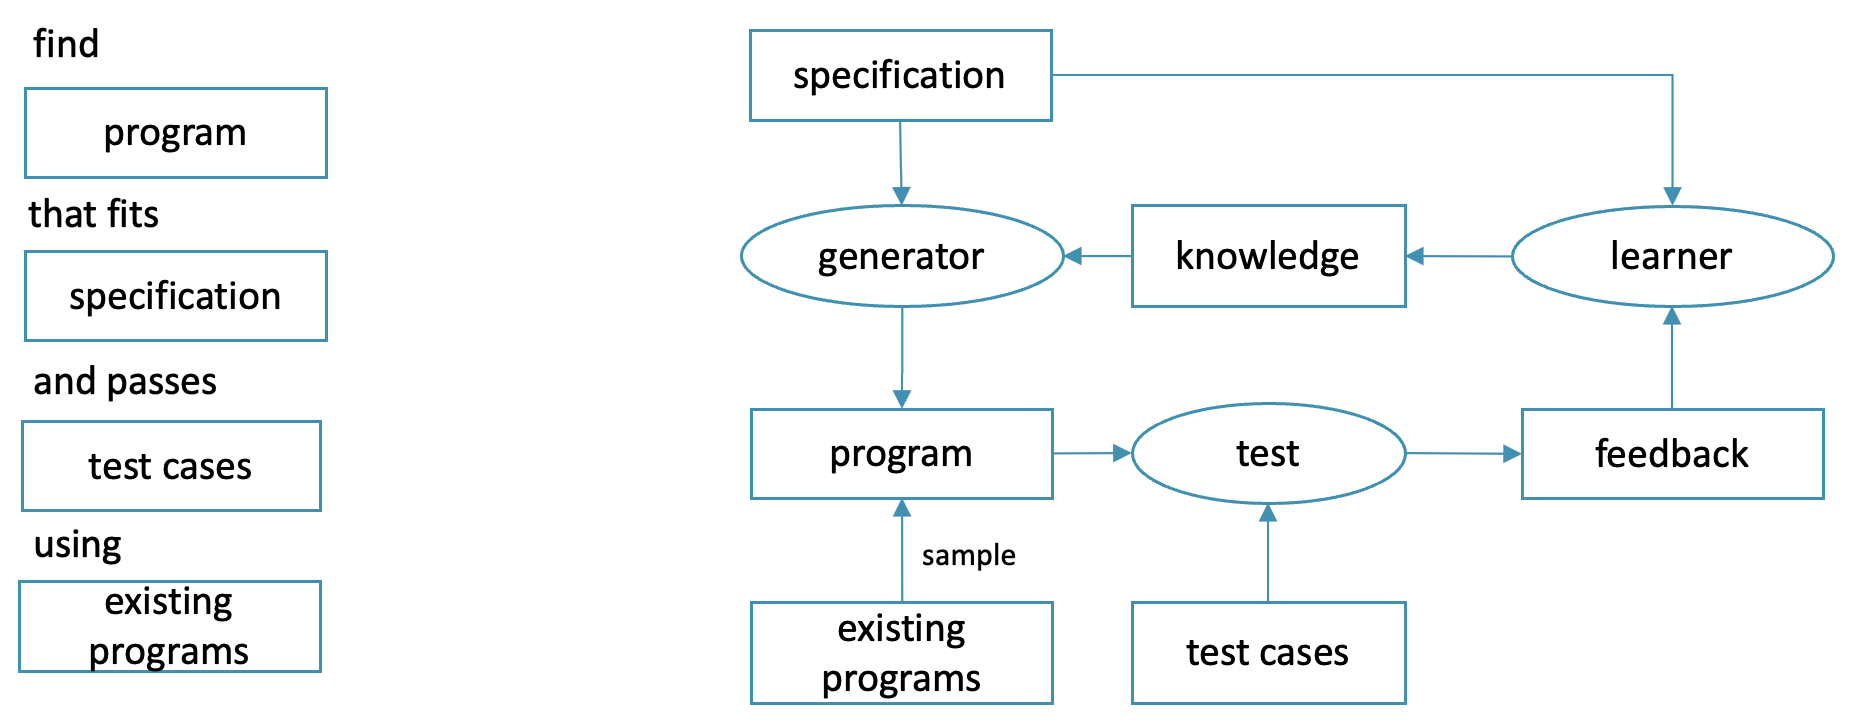
\includegraphics[width=\linewidth]{ap.png}
    \caption{Automatic programming system, schematic definition}
    \label{fig:ap}
\end{figure}

This definition is purposefully broad and includes, for example, the compiler \cite{penjamDeductiveInductiveMethods2003,patrickmckenzie[@patio11]GlibLineHave2023}: a program synthesis system that admits a specification in the form of a program in a high-level programming language designed for ease of use by humans and generates a program in a low-level programming language designed for ease of deployment on a computer.

\begin{figure}[H]
    \centering
    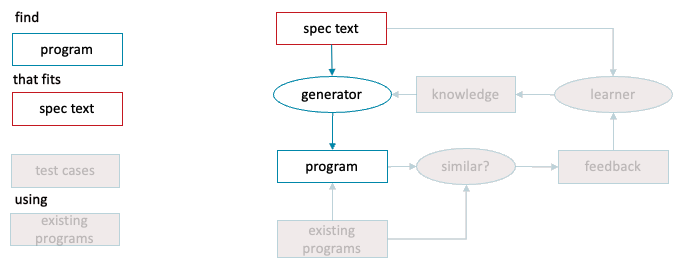
\includegraphics[width=\linewidth]{compiler.png}
    \caption{Compiler, schematic definition}
    \label{fig:compiler}
\end{figure}


The ambition of the field, however, extends far beyond compilers \cite{campbellAutomatedCodingQuest2020}.
The goal is to impose as few constraints as possible onto the \emph{specification} and ultimately automate the generation of programs for any free-form specification, such as a short textual \cite{zanLargeLanguageModels2023} prompt or a diagram \cite{koziolekLLMbasedControlCode2023}, even a hand-drawn sketch \cite{chatgptmodderChatgptCanNow2023}.

% TODO: examples for the above

\newpage
\section{Taxonomy of tasks \cite{liventsevTaxonomyAutomaticProgramming2023}}
\label{sec:taxonomy}

\paragraph{Code translation}

The humble compiler from section \ref{sec:quest} is an instance of a \emph{code translation} system: a \emph{program synthesis} system where the specification is given as text, either in a natural language (\emph{NL2Code translation} \cite{wangNaturalLanguageCode2023, zanLargeLanguageModels2023}) or in a programming language (\emph{code2code translation} \cite{radfordImprovingLanguageUnderstanding})
Code to natural language translation is studied as well \cite[section 5.1]{leDeepLearningSource2020}, but it is less common and out-of-scope for this work.
Intelligent conversational assistants (\href{https://chat.openai.com/}{ChatGPT}, \href{https://gemini.google.com}{Gemini}, \href{https://claude.ai/}{Claude}, \href{https://pi.ai/}{Pi}) with program synthesis functionality operate in the translation paradigm as they translate a text specification into code.

\begin{figure}[H]
    \centering
    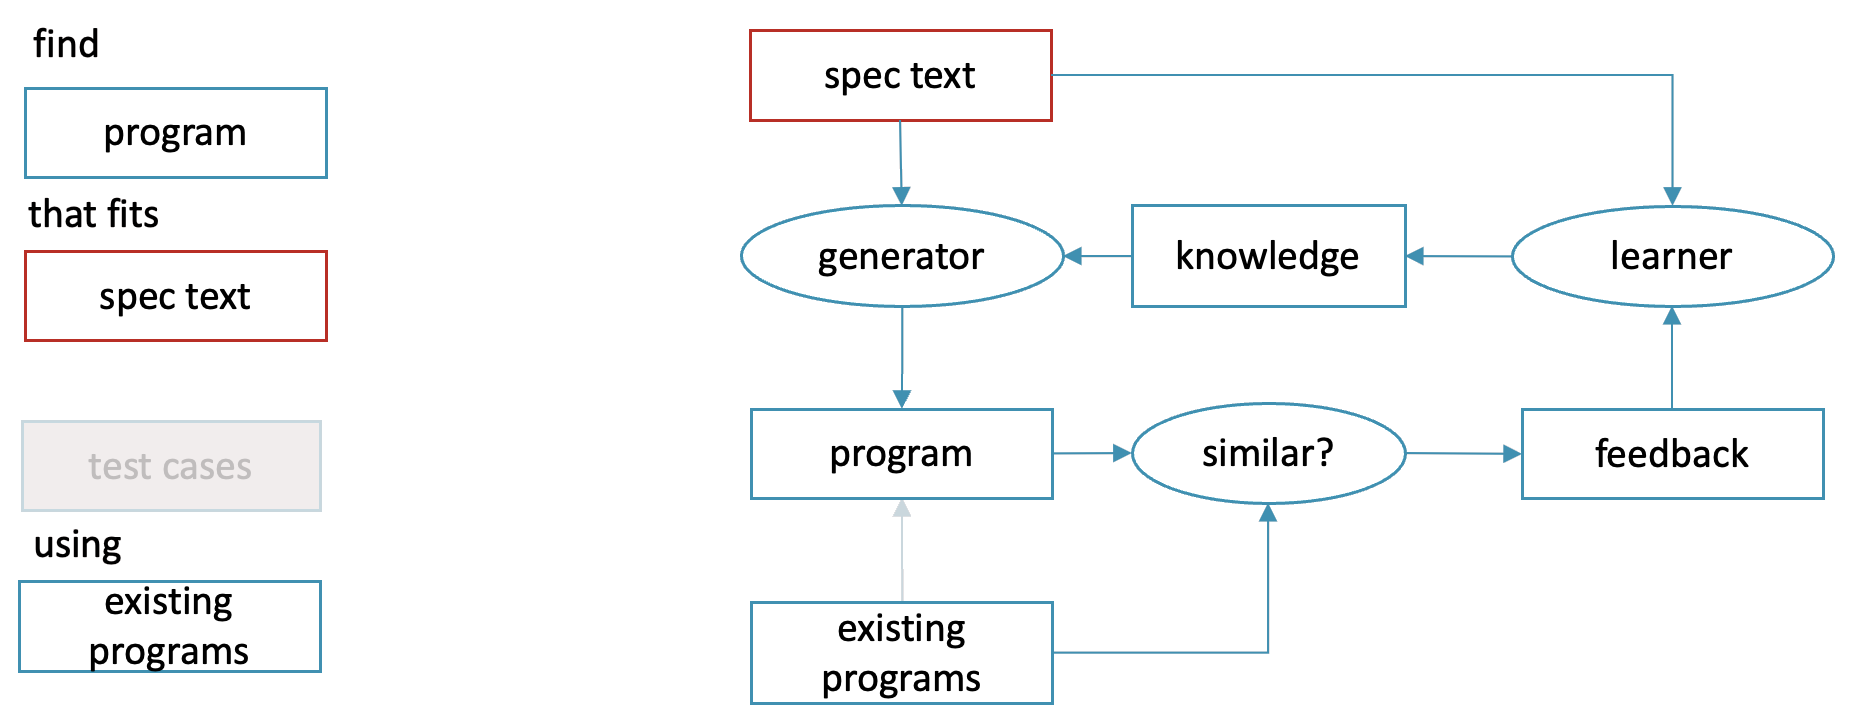
\includegraphics[width=\linewidth]{nl2ml.png}
    \caption{Code translation, schematic definition}
    \label{fig:nl2ml}
\end{figure}

\paragraph{Programming by example}

Another approach to specification is specifying the expected output of the program. Or, since in most interesting programs the output depends on the input, \emph{input-output pairs}. This task is known as \emph{programming by example} \cite{halbertProgrammingExample1984, psb2}.

\begin{figure}[H]
    \centering
    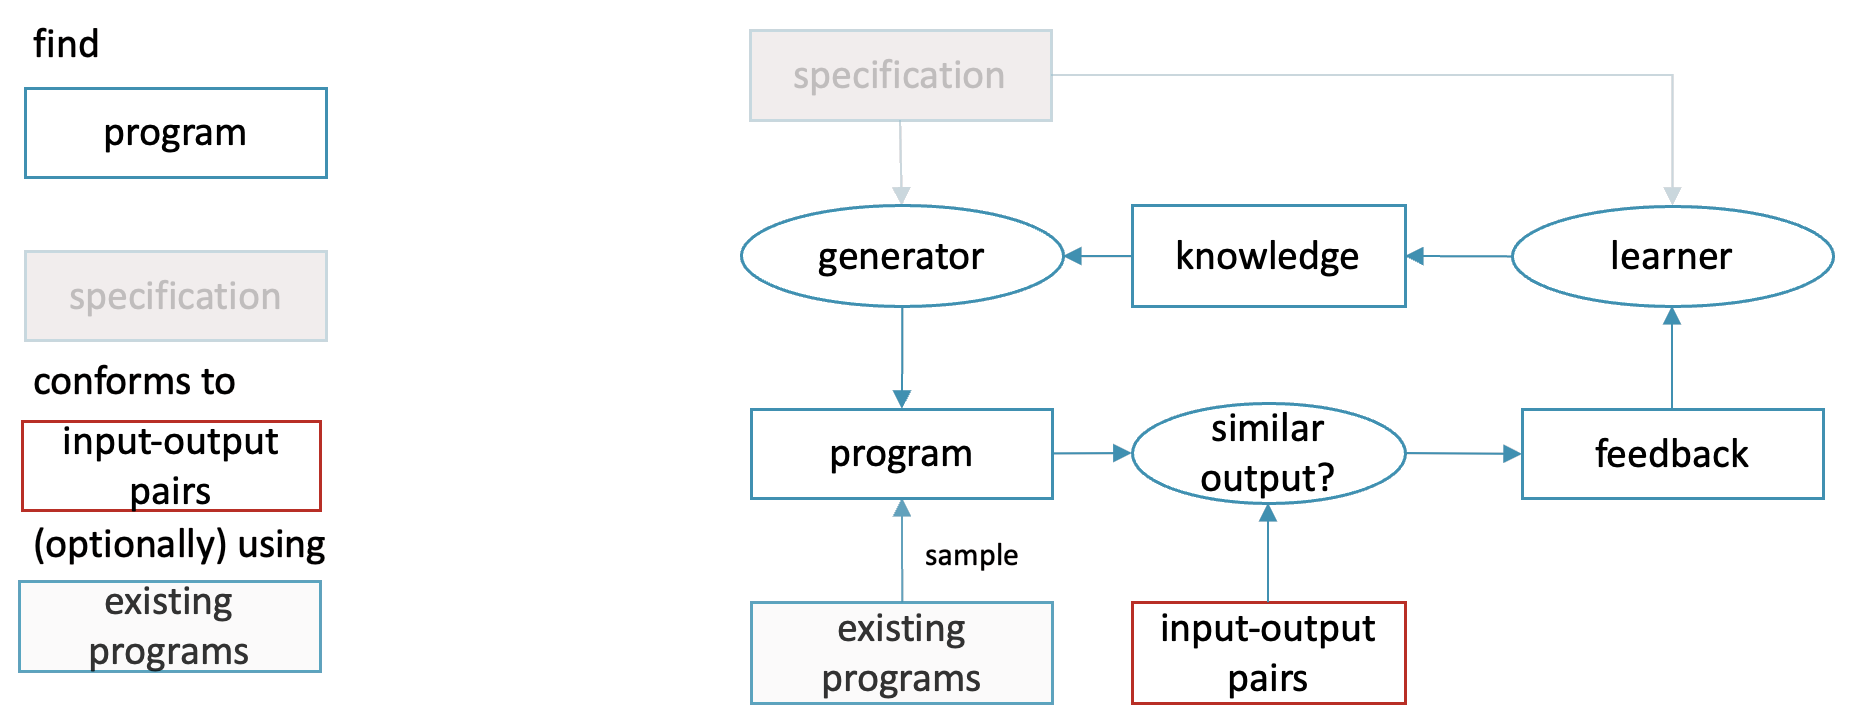
\includegraphics[width=\linewidth]{pbe.png}
    \caption{Programming by example, schematic definition}
    \label{fig:pbe}
\end{figure}

The goal of a programming by example system is to find a program $f$ such that $\outputvec=f(\inputvec)$ for a given vector of input-output pairs $(\inputvec,\outputvec)$. 
Note that this is exactly the definition of \emph{supervised learning}~\cite{cunninghamSupervisedLearning2008}.
Indeed, \emph{programming by example} is an unusual type of \emph{supervised learning}, one where the trained model is expressed as source code.

The prime application of \emph{programming by example} is \emph{data wrangling} tools such as Microsoft Excel \cite{gulwaniProgrammingExamplesandIts2016} where it is used as a data extrapolation tool: if a formula $f$ can be synthesized that satisfies $\outputvec=f(\inputvec)$, one can generate $\outputvec '=f(\inputvec ')$ for future values $\inputvec '$.
\emph{Programming by example} is also used in scientific domains to generate formulas that fit experimental observations, where it is known as \emph{symbolic regression} \cite{makkeInterpretableScientificDiscovery2022}.

\paragraph{PIRL}

Not every task, however, can be easily described with input-output examples. 
Take chess: it's relatively simple to evaluate the performance of a chess-playing program, but what are the \emph{correct} moves? 
That is simply not known in advance.
Given enough trial and error it's still possible to generate a correct program with such black box specification, a task known as \emph{Programmatically Interpretable Reinforcement Learning} \cite{pirl}.

\begin{figure}[H]
    \centering
    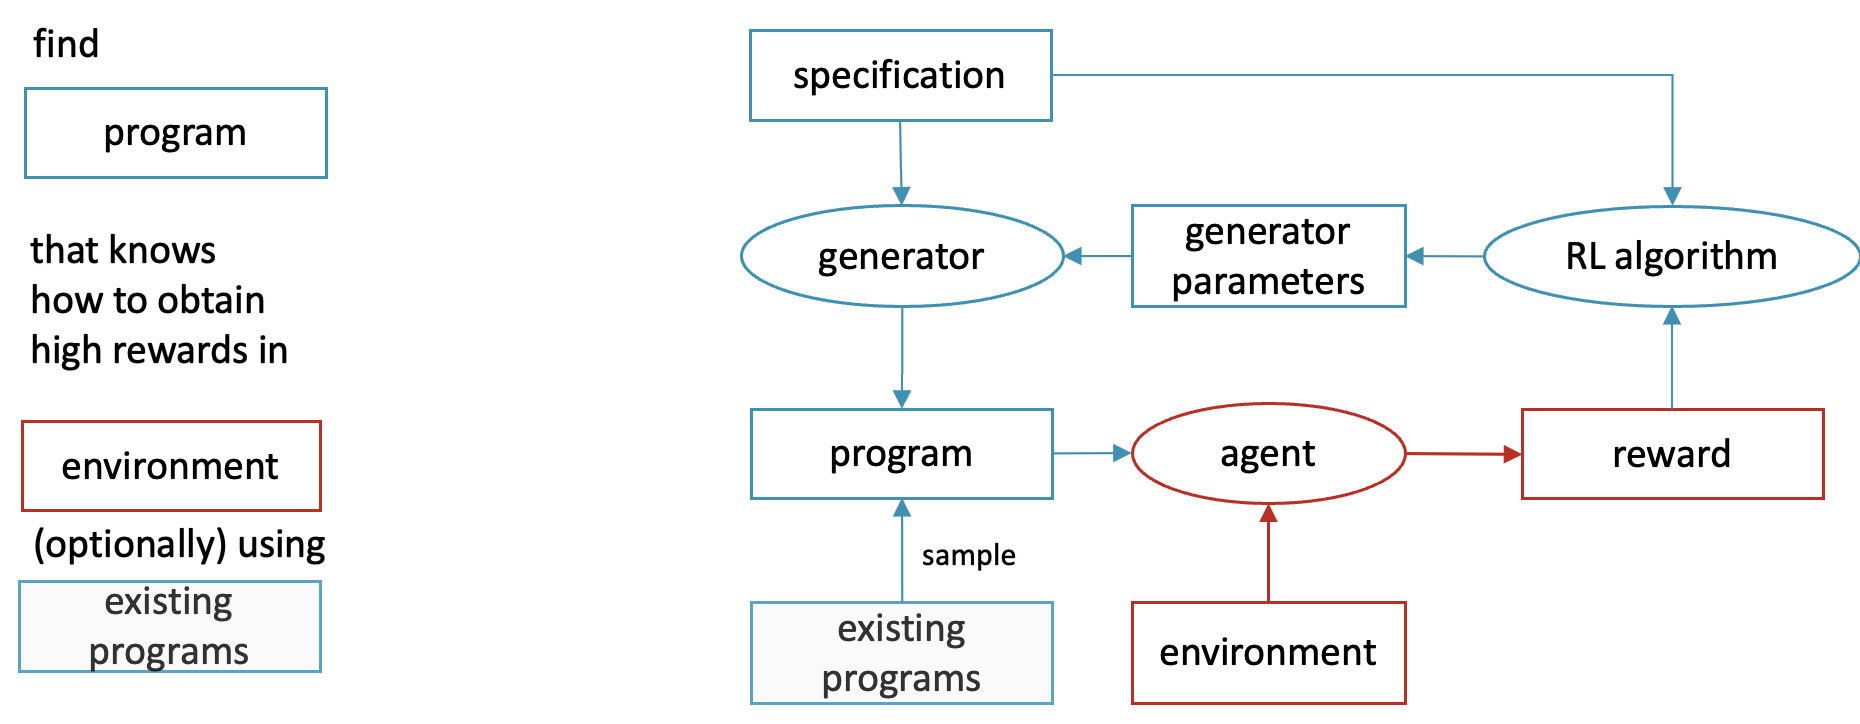
\includegraphics[width=\linewidth]{pirl.png}
    \caption{Programmatically Interpretable Reinforcement Learning, schematic definition}
    \label{fig:pirl}
\end{figure}

In this setting, a program gets generated and deployed in an environment that responds with positive and negative rewards. 
The most common formalism for such an environment as Partially Observable Markov Decision Process \cite{kramerjdavidrPartiallyObservableMarkov1964, spaanPartiallyObservableMarkov2012}: when at step $i$ the agent takes action $a_i \in \rlactionspace$ it has an impact on  the state of the environment $s_i \in \rlstatespace$ via distribution $\rlstatedistr$ of conditional probabilities of possible subsequent states. 
State is a latent variable that the agent cannot observe.
Instead, the agent can see an observation $o_i \in \rlobsspace$ which is a random variable that depends on the latent state via distribution $\rlobsdistr$.
$\rlactionspace$, $\rlstatespace$ and $\rlobsspace$ are sets of all possible actions, states and observations respectively.
Finally, at every step the agent observes a reward $\rlrewardf$

Given this limited toolset, without full (or any) prior knowledge of how the agent's actions influence the the environment (distributions $\rlstatedistr$ and $\rlobsdistr$), the agent has to come up with a strategy that will maximize $n$-step return $R_n=\sum_{t=i}^{n} r_t$ where $n$ is the agent's planning horizon. It is, in the general sense, a hyperparameter, however if an environment has a limit on how many steps an episode can last, it is reasonable to set $n$ equal to the step limit. 

\newpage
\section{Why not just use Machine Learning?}

As programmatically interpretable cousins of \emph{supervised learning} and \emph{reinforcement learning} respectively, \emph{Programming by example} and \emph{PIRL} are  used in settings where more traditional machine learning methods that don't involve code generation could also be used.
What are then the advantages conferred by this programmatic representation?

\paragraph{Expressiveness and performance}

Programming languages benefit from decades of research into making them \textcolor{accent}{expressive} - able to efficiently represent any algorithm one can design - and \textcolor{accent}{performant} - making those algorithms executable with minimal requirements of time and hardware.
Machine learning models don't have this advantage - they are designed to make the space of possible models easy to search and optimize in, often at the expense of expressivity and performance: an equivalent program typically solves the task better and faster than a machine learning model, to the point where representing algorithms as neural networks has become a setup of programmer humor \cite{JoelGrusFizz}.

In fact, \cite{JoelGrusFizz} underestimates the inefficiency of the neural approach, since in their neural network implementation an important part (output of text) is non-neural.
We correct for this and train a specialized language model for FizzBuzz, \emph{FizzBuzzLM}, benchmarking it against implementations of the same algorithm in major programming languages.

\begin{table}[H]
    \centering
    \begin{tabular}{r|r|l}
         Language & source, bytes & CPU runtime \\
         \midrule
         C & 321 & 340.3 µs ± 117.0 µs \\
         Clojure & 178 & 507.2 ms ± 6.5 ms \\
         C\# & 289 & 60.4 ms ± 4.8 ms \\
         Go & 295 & 966.5 µs ±  93.2 µs \\
         Haskell & 213 & 16.1 ms ± 0.4 ms \\
         Java & 403 & 28.9 ms ± 0.6 ms \\
         JavaScript & 162 & 30.1 ms ± 0.4 ms \\
         Python & 192 & 44.9 ms ± 0.6 ms \\
         Rust & 307 & 573.5 µs ± 114.3 µs \\
         FizzBuzzLM & 13177 & 853.2 ms ± 6.8 ms\footnote{GPU (NeuralEngine) runtime was even slower, at 1.596 s ± 0.037 s}
    \end{tabular}
    \caption{Performance charecteristics of different FizzBuzz implementations}
    \label{tab:my_label}
\end{table}

We can see that the programming language implementations are somewhat faster than \emph{FizzBuzzLM} and much more expressive with at least \emph{FizzBuzzLM} 2 orders of magnitude behind the true Kolmogorov complexity \cite{kolmogorov} of the problem.
The only reason why these performance costs are accepted is that it's easier to implement optimization in the space of possible neural network parameters than in the space of possible programs. 
When the problem of optimal program synthesis is solved, it becomes the "best of both worlds" approach: data-driven and trainable, but using an expressive an performant representation.
 
\paragraph{Import and export of knowledge}

Programs as a representation for decision-making of a model have a chance to become the \emph{lingua franca} \cite{samarinLinguaFranca1987} for representing decision processes as they can be understood both by a wide variety of machine learning and artificial intelligence systems and by humans, enabling humans and robots trying to tackle the same problem to learn from each other.

\begin{figure}[H]
    \centering
    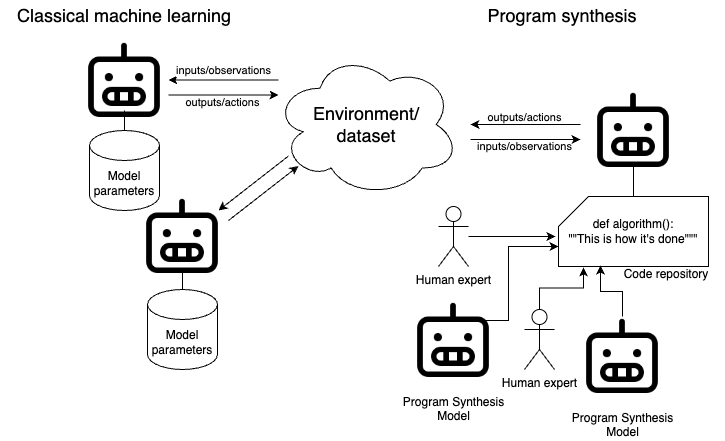
\includegraphics[width=\linewidth]{mlvsautocode.png}
    \caption{Program synthesis allows for knowledge sharing}
    \label{fig:mlvsautocode}
\end{figure}

The search in a space of possible programmatic solutions to a problem can be initialized with an existing program that has been developed by an expert in the field (perhaps with the  use of AI tools), thus \textcolor{accent}{importing existing knowledge} from previous efforts of solving the same problem.
This process is not dissimilar to what is known in deep learning as \emph{fine-tuning}: initializing the optimization process of model parameters with a model already trained on a similar task, but it has the additional advantage that the initial code can be generated by a model of a completely different architecture or by a human.

After the search process has been concluded, all of the knowledge incorporated into the resulting system can be \textcolor{accent}{examined and verified}. 
Unlike the black-box model, the approach makes it trivial to answer questions like "Does this model include factor X in its decision-making on topic Y?".
This offers us an additional way of verifying the decision system before its final deployment. 
And, unlike the numerous post-hoc methods of machine learning interpretability \cite{linardatosExplainableAiReview2020}, this approach involves a strong guarantee that the explanation does not diverge from the behavior.

Of course, the external observers of a program synthesis system can be not only teachers, but also students. 
Even if the resulting program is never deployed, one can read it and \textcolor{accent}{export the knowledge} and incorporate it into future systems, as well as textbooks and other didactic materials for humans.

\newpage
\section{Broader impacts}

\epigraph{The Future's So Bright, \\ I Gotta Wear Shades}{Timbuk 3}

\paragraph{Capability}

The \emph{expressivity and peformance} of programming languages can lead to \emph{decision support systems}, also known as \emph{digital assistants}, that are more capable, better able to make predictions and provide advice.

The ability to \emph{import, verify and export knowledge} into or out of a decision suport system can reduce or even eliminate the amount of \emph{knowledge silos} that exists in the ecosystem of these agents, where each separate system has been trained on some data set of its own and some expert knowledge of its own and each incorporates some small part of existing knowledge about the field. 

Insufficient capability in digital assistants can be a major safety risk, especially when they're deployed fully autonomously. For example, misidentification of obstacles in autonomous driving \cite{sheebajoiceObstacleDetectionSafe2023} or wrongful diagnosis in healthcare \cite{wintersDiagnosticErrorsIntensive2012} can be a matter of life and death.

\paragraph{Alignment}

Highly capable digital assistants present their own family of safety risks. 
If perverse incentives are present in the optimization goals of the decision system, then a highly capable decision system can bring about harmful situations intentionally.
Most optimization targets are imperfect proxies of intended outcomes. 
An optimization process can thus \emph{game} (\emph{hack}) the metrics and achieve negative outcomes, despite technically improving the metrics.
Common types of \emph{reward hacking} \cite{skalseDefiningCharacterizingReward2022} include:
\begin{description}
    \item[reward tampering] \cite{everittRewardTamperingProblems2021, skalseInvariancePolicyOptimisation2023} - acting on the reward mechanism directly, i.e. disabling sensors involved in performance evaluation or writing more flattering documentation.
    \item[adverse selection] - selectively solving subtasks that are easier to solve even if they happen to be more important.
\end{description}

To give a real world example, both phenomenons have been observed in Healthcare: \cite{shenSelectionIncentivesPerformance2003} find that incentives can lead to the most severely ill patients being less likely to receive care. \cite{fairbrotherImpactFinancialIncentives2001, ImpactPhysicianBonuses, roskiImpactFinancialIncentives2003} find that metrics are sometimes improved by better documenting the incentivized results, not improving them.
\cite{longFairnessMachineLearning2021} notes how misguided fairness metrics incentivize decision systems to intentionally harm people from healthier demographic groups in order to advance equality of outcomes ("equity").

These issues are present in society \cite{nestianPerverseIncentiveGeneral2017} with or without artificial intelligence, they are studied in economics under the umbrella of the \emph{principal agent problem} \cite{pandaAgencyTheoryReview2017}. 
However, powerful optimization algorithms have potential to exacerbate those issues \cite{hadfield-menellIncompleteContractingAI2019}. 
And while the first line of defense is, of course, improving the incentives, one can be skeptical as to whether the incentives can ever represent their designers' intentions perfectly.

In fact, the instrumental convergence theory \cite{benson-tilsenFormalizingConvergentInstrumental} posits that perverse incentives are inherent to any reinforcement learning context, because optimizing for any goal can be aided by increasing the amount of control over one's environment the agent has, and thus any optimization of agents creates incentives to maximize their own power and control. 
First introduced in science fiction \cite{clarke2001SpaceOdyssey2016, ellisonHaveNoMouth1967, jonesColossus2019}, this is now an active area of technical research \cite{jiAIAlignmentComprehensive2024}.
Estimates of the potential dangers of misaligned artificial intelligence range from non-trivial to existential \cite{mcleanRisksAssociatedArtificial2023}.

The interpretability afforded by the program synthesis approach provides a second line of defense against perverse incentives, namely examining the control program and trying to establish whether any of the modules in that program are attempting to game the optimization metrics, manually or with the use of AI tools.

\begin{figure}[H]
    \centering
    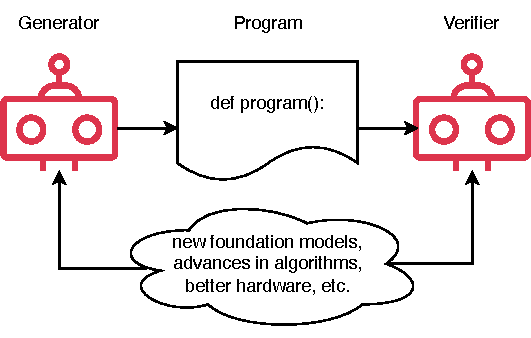
\includegraphics{PSAlign.drawio}
    \caption{Program Synthesis as an alignment methodology}
    \label{fig:ps-as-alignment}
\end{figure}

As the field of artificial intelligence advances, this advances both the generative tools and the verification tools, thus making program synthesis a viable approach to scalable oversight \cite[section 5]{amodeiConcreteProblemsAI2016}.

\paragraph{Human-Robot Teams}

Transparency is a foremost principle of effective teamwork: every member of the team is supposed to know what and why every other member is doing. 
This principle is supported by the study of human teams \cite{bagPEERTRANSPARENCYTEAMS2012a, solomonInferenceTransparencyEffective2021} and human-robot teams \cite{ezenyilimbaImpactTransparencyExplanations2022, guznovRobotTransparencyTeam2019, holderDesigningBiDirectionalTransparency2021, lakhmaniExploringEffectCommunication2019, lakhmaniProposedApproachDetermining2016, mercadoIntelligentAgentTransparency2016, ososkyDeterminantsSystemTransparency2014, panganibanTransparencyAutonomousTeammates2020, ronconeTransparentRoleAssignment2017} alike.
Some literature in Human-Robot teams takes inspiration \cite{shivelyCrewResourceManagement2018} from teamwork research in aviation where studies into the common causes of incidents and accidents \cite{chidesterPersonalityFactorsFlight1990, chidesterPilotPersonalityCrew1991, smithSimulatorStudyInteraction1979} have been used to formulate core principles of Crew Resource Management, such as "Verbalize Verify Monitor".
And as more automation is introduced in aviation, the modern cockpit itself can be seen as a human robot team.
Same is true of an operating theater with a robot assistant \cite{weerarathnaHumanRobotCollaborationHealthcare2023} or a doctor using a clinical decision support system \cite{castilloConsiderationsSuccessfulClinical2013, mooreIntroductionClinicalDecision2011, osullivanDecisionTimeClinical2014, purcellWhatMakesGood2005, sakallarisClinicalDecisionSupport2000, selfClinicalDecisionSupport2008, stangeThisIssueClinical2011, wrightClinicalDecisionSupport2009}

The lack of transparency is an important roadblock for integration of black box decision systems in safety critical domains: when conflict arises between the opinion of the expert and the opinion of the system, a black box system offers no additional information for the resolution of the conflict. 
A program, on the other hand, offers the experts a way to explicitly examine why a certain advice is given and use this information to take or not take the advice into account. 
Consequently, a black box system can only be used to completely replace a certain job - any setting where a collaboration is required between a human and decision system requires some degree of transparency that can be afforded by technology like program synthesis. 
This ensures synergistic decision-making where the analysis of every participant is taken into account of the final decision.

\paragraph{Compliance}

Both individual organizations and regulatory authorities often impose requirements onto their decision systems that assume their transparency. 
An audit has to be able to establish whether the system displays any illegal patterns such as a violation of established clinical protocol in healthcare or unauthorized discrimination in insurance and lending. 
Such requirements have had a chilling effect on the real world deployment of deep learning systems. 
A program, on the other hand, can be audited and proven to be compliant. 
Program synthesis can thus bring all the advantages of big data-driven systems into such fields without necessitating a regulatory reform.

\paragraph{Privacy}

The ineffiency of inference of current machine learning models is (along with competitive pressures) a core reason of the "cloudification" of artificial intelligence: as of late 2023, the most powerful products of machine learning \cite{achiamGpt4TechnicalReport2023} are distributed as remote services that can be interacted with, but not fully copied, via the Internet.
Asking a state of the art decision support system for advice means sending the (potentially sensitive) request to the model provider and making both requests and responses known to said provider \cite{PrivacyPolicy}.
Programs, in contrast, are easier to distribute and performant enough to run on most devices most of the time.
The advent of program synthesis can pave the way to more privacy-preserving decision support: even if the generative model remains in the cloud, one can first use the model to synthesize the program, download it and then submit the sensitive data to the program locally.

% Add a point about IP

\paragraph{Scientific discovery}

Lastly, export of knowledge out of a automatic programming system can be a powerful tool of scientific discovery. 
Symbolic regression is already widely used in physics in order to find formulas that fit experimental results \cite{angelisArtificialIntelligencePhysical2023, tenachiDeepSymbolicRegression2023}. 
In fact, it is not unreasonable to claim that physics \emph{is} a set of symbolic regression problems \cite{udrescuAIFeynmanPhysicsinspired2020}, historically solved manually, but increasingly with some application of algorithms. 
The same can be said about biology \cite{chenRevealingComplexEcological2019}, economics \cite{claveriaAssessmentEffectFinancial2017, lianModelingForecastingPassenger2018, panInfluentialFactorsCarbon2019, truscottDetectingShadowEconomy2011, truscottExplainingUnemploymentRates2014, yamashitaCustomizedPredictionAttendance2022} or any field that develops formulas based on series of empirical observations.

%----------------------------------------------------------------------------------------
%\newpage
%\chapter{The State of the Art}\label{ch:autocode-sota}
%\section{Existing simulators}
\label{sec:existing}

\subsection{simglucose}
\label{sec:simglucose}

\begin{figure}
    \centering
    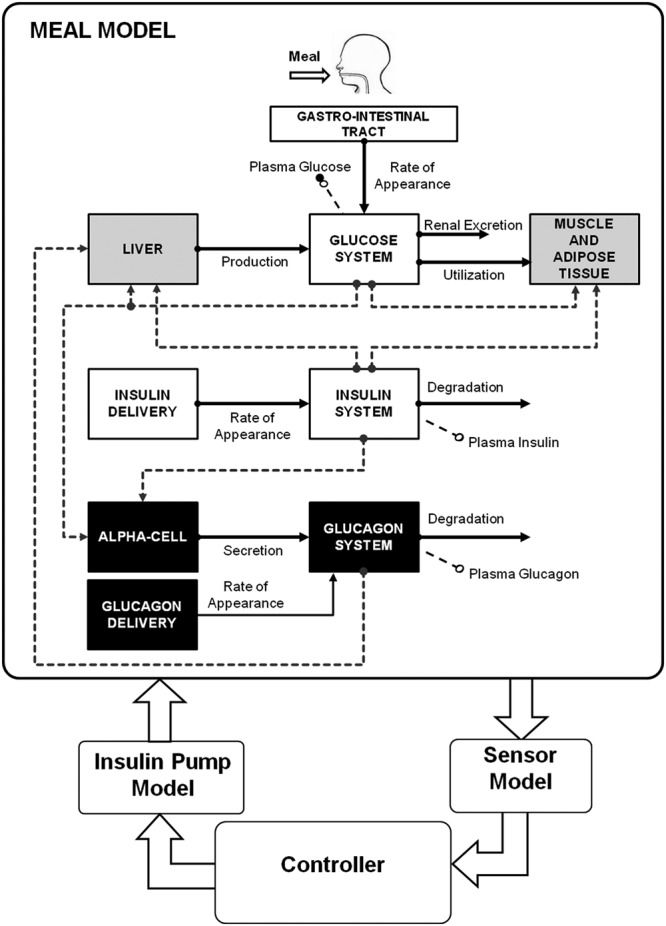
\includegraphics[width=\linewidth]{uvapadova.jpg}
    \caption{UVA/PADOVA equations, visualised}
    \label{fig:uvapadova}
\end{figure}

UVA/Padova \cite{sim-diabetes-fda} is a set of equations used to model type 1 diabetes.
The equations, outlined on figure \ref{fig:uvapadova}, were developed by clinical experts and validated on a dataset of 32 people aged 38 ± 12 years.
It is widely used in Healthcare and even approved in the United States as a replacement for clinical trials.
It provides $p_o(o | s, a)$ and $p_s(s_\text{next} | s_\text{prev}, a)$ (see section \ref{sec:scope}), so to be a full-fledged Markov Decision Process it only need $p_r(r|s,a)$.
\cite{simglucose} solves exactly that by adding a reward function based on diabetes risk index as defined in \cite{diabetesrisk} to the UVA/Padova simulator, providing a Reinforcement Learning environment for type 1 diabetes.

\subsection{GYMIC}
\label{sec:gymic}

\subsubsection{Scope}
GYMIC \cite{gymic} is, unlike the previous examples, a fully data-driven simulator. 
It harnesses a subset of MIMIC \cite{mimic} dataset to address on one of the most challenging problems in emergency care - sepsis.
The authors intentionally limit their scope to just sepsis in order to simplify the modelling task as well as because sepsis prevention has been identified as an area where doctors would particularly benefit from electronic decision support \cite{sepsis-motivation1,sepsis-motivation2}.

\subsubsection{Prediction model}
The prediction model of GYMIC simulator is defined as a solution to the following autoregression task:
\begin{enumerate}
    \item A clinical history is a sequence of $(s, a)$ tuples
    \item $a \in 0,\dots 24$ is one of 25 possible vasopressor or intravenous fluid interventions - a cartensian product of 5 types of interventions and 5 dosage quantiles. 
    \item $s \in R^{46}$ is the patient's state at the moment this intervention was administered.
    \item Predict the conditional state distribution $p_s(s_t, a_t | s_{t-1},s_{t-2},\dots,s_1)$
\end{enumerate}

The dataset of clinical histories is produced by a preprocessing algorithm combining together all clinical records from MIMIC that relate to sepsis patients.

Autoregressive tasks of this nature arise in many fields like stock market prediction \cite{stonks1,stonks2} or language modelling \cite{langmodels} where state of the art solutions can be found.
The authors of \emph{GYMIC} solve it with an LSTM \cite{hochreiterLongShorttermMemory1997} neural network with 2 additional dense layers attached, see figure \ref{fig:gymic} for the diagram.
Faced with some of the mode collapse issues described in section \ref{sec:gymic-results} the authors also experimented with semi-supervised learning \cite{semi-supervised}: they trained a variational autoencoder \cite{vae} on all patient states to replace the 46-vector representations of patient state $s$ with learned representations from the latent space of the VAE $\text{encoder}(s)$.
The issues persisted.

\begin{figure}
    \centering
    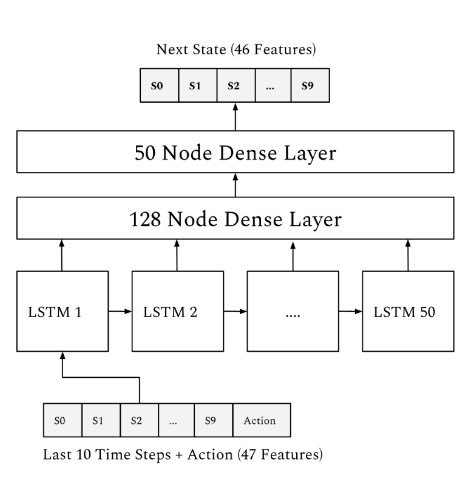
\includegraphics[width=\linewidth]{gymic.png}
    \caption{Neural architecture of GYMIC}
    \label{fig:gymic}
\end{figure}

\subsubsection{Reward model}

Highlighting the gravity of contracting sepsis, \emph{GYMIC} has only 2 outcomes: patient is discharged from intensive care or patient dies.
Its reward model reflects that, giving the agent a large positive or negative reward at the end of the episode, depending on the outcome.
However, in order to lower the difficulty of the simulator (delayed gratification makes training significantly harder \cite{delayedgrat-humans, delayedgrat-ai}) an additional reward is provided during the episode, based on the evolution of the patient's SOFA score \cite{sofa} - a commonly used measure of sepsis severity:

\begin{multline}
r\left(s_{t}, s_{t+1}\right)=C_{0} \mathbb{1}\left(s_{t+1}^{\mathrm{SOFA}}=s_{t}^{\mathrm{SOFA}} \& s_{t+1}^{\text {SOFA }}>0\right) + \\ +
C_{1}\left(s_{t+1}^{\mathrm{SOFA}}-s_{t}^{\mathrm{SOFA}}\right) + 
C_{2} \tanh \left(s_{t+1}^{\text {Lactate }}-s_{t}^{\text {Lactate }}\right)
\end{multline}

A third reward component is proposed to negatively reinforce action severity and encourage the agent to use low doses of drugs - an instance of \emph{confirmation bias} as discussed in section \ref{sec:bias}, but a necessary step given the issues in section \ref{sec:gymic-results}.

\subsubsection{Results and issues}
\label{sec:gymic-results}

Unfortunately, the experiments performed by the authors of \emph{GYMIC} indicate extreme overfitting.
Due to \emph{sampling bias} and simply inadequate size of the dataset there are treatments that have only occurred a few times in the training data and have always resulted in a positive health outcome.
In \emph{GYMIC} these treatments are silver bullets that guarantee a successful outcome while in real life they are risky and potentially very harmful.


\newpage
\chapter{BF++: a Novel Language for PIRL}\label{ch:autocode-dsl}
\citeself{chapter}{liventsev2021:bf}

\section{BF++}
\label{sec:language}

\paragraph{BF syntax}
\label{sec:bf}

Abolafia {\sl et al} \cite{abolafiaNeuralProgramSynthesis2018} picked BF\footnote{Brainfuck} \cite{brainfuck} as their language for program synthesis for the following reasons:
\begin{itemize}
    \item In industry-grade programming languages like Python or Java program code can contain a very large variety of characters since any of the 143859 Unicode \cite{allenUnicodeStandard2012} characters can be used in string literals. In BF, however, only 8 characters can be used: they can be one-hot-encoded with vectors of size 8. 
    \item BF's simple syntax means that an arbitrary string of valid characters is likely to be a valid program. 
    In more complex languages, most possible strings result in a syntax error. 
    A generative model being trained to write programs in such a language risks being stuck in a long exploration phase when all the programs it generates are invalid and it has no positive examples in the dataset.
    \item Despite all of the above, it is a Turing-complete language.
\end{itemize}

The simplicity of the language also means that it is relatively easy to develop a compiler that translates programs from an industry-standard programming languages like Java and Python to BF thus making use of the expert knowledge existing in those languages. 

In the current chapter, we introduce an extended version of the original BF language, BF++. As explained below, the extensions to the original BF syntax are particularly useful in the RL use cases. 

BF's runtime model is inspired by the classic Turing Machine \cite{turing}: at any point during the program's execution, the state of the program consists of:

\begin{itemize}
    \item An infinite\footnote{If you happen to be executing a BF program on a computer with finite memory, the tape will be finite due to your hardware limitations.} tape of cells $T$ where each cell holds an integer number.
    \item A \textit{memory pointer} $p_T$ that points to a certain cell in the tape (\textit{active cell} $T^{p_T}$).
    \item A string of characters $C$ that represents program code.
    \item A \textit{code pointer} $p_C$ pointing to a character about to be executed.
\end{itemize}

The code pointer starts at the first character, then this character gets executed and the pointer is incremented (moved to the next character).
There are 8 possible characters:

\begin{description}
\item[\texttt{>}] Move the memory pointer one cell right. $p_T := p_T + 1$
\item[\texttt{<}] Move the memory pointer one cell left. $p_T := p_T - 1$
\item[\texttt{+}] Increment the \textit{active cell}. $T^{p_T} := T^{p_T} + 1$
\item[\texttt{-}] Decrement the \textit{active cell}. $T^{p_T} := T^{p_T} - 1$
\item[\texttt{.}] Write $T^{p_T}$ from the \textit{active cell} to the \textit{output stream}\footnote{The definition of input and output streams is purposefully underspecified, it may depend on the particular implementation.}
\item[\texttt{,}] Read $x$ from the \textit{input stream} to the \textit{active cell}. $T^{p_T} := x$
\item[ \texttt{[} ] If the \textit{active cell} $T^{p_T} = 0$, jump (move $p_C$) to the matching $]$.
\item[ \texttt{]} ] If the \textit{active cell} $T^{p_T} \neq 0$, jump (move $p_C$) to the matching $[$
\end{description}

[ and ] commands constitute a loop that will be executed repeatedly until the \textit{active cell} becomes zero.
They are also the only way to write a BF program with a syntax error: a valid BF program is one that doesn't contain non-matching [ or ]

% TODO: example?

\paragraph{Negative values}

In \textbf{BF} memory cells $T^i$ hold non-negative values only.
In \textbf{BF++} $T^i \in \mathbb{Z}$, a negation operator \texttt{\~} is introduced and operators \texttt{[]}are redefined to loop while the \textit{active cell} is non-positive, i.e.

\begin{description}
\item[ \texttt{\~} ] If the \textit{active cell} $T^{p_T} := - T^{p_T}$.
\item[ \texttt{[} ] If the \textit{active cell} $T^{p_T} \geq 0$, jump (move $p_C$) to the matching $]$.
\item[ \texttt{]} ] If the \textit{active cell} $T^{p_T} < 0$, jump (move $p_C$) to the matching $[$
\end{description}

This decision was taken because negative observations are common in control problems (see section \ref{sec:bfpp-experiments}) as is branching on whether the observed value is positive or negative. 

\paragraph{Non-blocking action operators}
\label{sec:queue}

% TODO: cite some literature
% We're not the first people tackling these challenges, right?

The main issue of \textbf{BF} as a language for Reinforcement Learning is its input-output system.
It assumes that the program can freely decide on the relative frequency of inputs to outputs.
For example, the following program

\begin{center}
\begin{lstlisting}
+[.....,]
\end{lstlisting}
\end{center}

inputs 5 integers, outputs the 5th character it read, then goes back to the beginning and proceeds indefinitely outputting every 5th character it inputs.
Thus it assumes a 5:1 frequency of inputs to outputs.
If we simply assume that inputs are observations and outputs are actions, such program will not be able to operate in a POMDP environment where I/O frequency is fixed at 1:1 and the agent that has made an observation has to act before it can make the next observation.
In other words, operators \texttt{.} and \texttt{,} are blocking: \texttt{.} stops program execution and waits until new input is received to resume execution, \texttt{,} stops program execution and waits until there is an opportunity to act in the environment.

To address this, in \textbf{BF++} \texttt{.} operator is non-blocking.
It outputs the current value of the active cell by placing it at the bottom of the \textit{action queue} $S$ - a sequence of integer numbers that represent actions the program is planning to take in the environment. We also introduce a non-blocking operator \texttt{!} that places $T^{p_T}$ on top of the action queue.

\begin{equation}
    \begin{array}{cc}
         . & S := S^\frown (T^{p_T}) \\
         ! & S := (T^{p_T})^\frown S
    \end{array}
\end{equation}

where $\frown$ denotes concatenation of tuples

The program can thus decide by using \texttt{.} or \texttt{!} whether the newly added action takes precedence over ones already in the queue.
As soon as an opportunity to act arises, the top of the action queue (item $S^1$ or several items $S^1,S^2,\dots$, see section \ref{sec:envs}) defines which action the program takes and is then removed from the queue. 
If $S^k$ does not exist (the queue is empty or shorter than $k$) default value of $S^k=0$ is assumed.

\texttt{,} operator, on the other hand, is blocking. 
Thus its function is more important than just reading an observation into memory.
Executing \texttt{,} is when the program moves to the next step of POMDP.

\paragraph{Virtual comma}
\label{sec:virtualcomma}

% TODO: fading text for virtual commas

The system where the only way to proceed to the following iteration is the \texttt{,} operator, naively implemented, means that to be successful in any POMDP environment, a program has to contain an infinite loop with a \texttt{,} operator.
Any program that has a finite number of \texttt{,} steps will terminate prematurely in an environment that supports arbitrarily long number of iterations.
Since we originally set out to develop a language where most random programs would be valid, this had to be addressed.

We decided to turn any \textbf{BF++} program into an infinite loop with a \texttt{,} operator by default:
\begin{enumerate}
    \item Every \textbf{BF++} program starts with a virtual \texttt{,} operator at address $p_C = -1$: it is executed before all operators in the code of the program, they are indexed starting from $p_C = 0$
    \item When the code pointer $p_C$ reaches the end of the program it loops back to the virtual comma $p_C := -1$
\end{enumerate}

Due to the virtual comma, every program starts executing with the initial observation already stored in memory and available for branching/decision-making.

\paragraph{Observation discretization}
\label{sec:observe}

Another issue complicating applications of \textbf{BF} to Reinforcement Learning is that since its memory tape holds only integer numbers its inputs and outputs have to be integer as well.
And this issue cannot be fixed simply by replacing an integer tape with a tape of floating point numbers as \textbf{BF}'s only operations for manipulating numbers are \texttt{+} and \texttt{-} - increment and decrement.
Non-integer action and observation spaces are fairly common in reinforcement learning tasks hence \textbf{BF++} implements coercion mechanisms for reading and writing continuous vectors into discrete memory.

We assume that the vector observation space $O$ is a hypercube defined as an intersection of $n$ separate scalar observation spaces $O^k$ such that 
\begin{equation}
 o_1 \in O_1^k,o_2 \in O_2^k,\dots,o_n \in O_n^k \Leftrightarrow (o_1,o_2,\dots,o_n) \in O  
\end{equation}

This assumption theoretically excludes some possible observation spaces, but almost all POMDP tasks discussed in the research literature and all OpenAI Gym tasks conform to this assumption.

To write an observation onto the memory tape we the observation vector of size $n$ is aligned with memory cells $T^{p_T},T^{p_T+1},\dots,T^{p_T+n-1}$ and turned into an integer with the use of $d$ discretization bins.

\begin{equation}
\label{eq:discretization}
T^{p_T+k-1} := \min_{\omega \in 1,\dots d | o^k < \tau^k_\omega} \omega
\end{equation}

If $O^k$ is an interval $O^k=[o_{low}, o_{high}]$, it is split into discretization bins evenly, as in eq. \ref{eq:static-thresholds}:

\begin{equation}
\label{eq:static-thresholds}
\tau_\omega = \begin{cases}
o_{low}+\frac{o_{high}-o_{low}}{d}\omega, \omega=1,2,\dots,d-1 \\
+\infty, \omega=d 
\end{cases}
\end{equation}

\begin{figure}[htb]
    \centering
    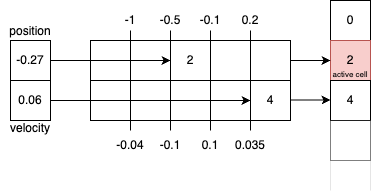
\includegraphics[width=0.8\linewidth]{observ.png}
    \caption{Fluid discretization example in Mountain Car}
    \label{fig:obs}
\end{figure}

Some environments, however, have unbounded observation spaces $O^k=(-\infty;+\infty)$, $O^k=(-\infty;o_{high}]$,  $O^k=[o_{low};+\infty)$.
This spaces are challenging because the formal description $O^k$ does not in any way reflect the actual underlying distributions of observations.
It can be the case, for example, that $O^k=(-\infty;+\infty)$ but most observations found in the environment fall in the interval $O^k=[42;43]$.
For such observation spaces, \textbf{BF++} uses a \textit{fluid discretization} system that learns the true distribution of observations online. The idea was inspired by a work of Touati {\sl et al} \cite{adaptivediscretization}, although, they assumed that $O^k$ has a finite diameter and didn't support unbounded observation spaces.
Initial thresholds $\tau_\omega$ can be arbitrary.
With each new observation, thresholds $\tau_\omega$ are readjusted so that among $h$ prior observations, roughly $\omega$ out of $d$  observations are lower values that $\tau_\omega$:

\begin{equation}
\underset{\tau}{\text{minimize}} \sum_{\omega \in 0,1,\dots d} |\frac{\omega}{d} - \frac{\sum_{i' \in i-h,i-h+1,\dots,i-1} \mathbb{I}(o_{i'}^k < \tau_\omega)}{h}|
\end{equation}

To solve this optimization problem, one has to sort previous $d$ observations in ascending order so that 

\begin{equation}
    \text{sort}: \{o_i | i \in i-h,i-h+1,\dots,i-1\} \longrightarrow \{ s_i | i \in 1,2,\dots,h \}
\end{equation}

is such a bijection that $s_1 < s_2 < \dots < s_h$ holds and set

\begin{equation}
    \tau_{\omega} = s_{\lceil \frac{\omega}{d} h \rceil}
\end{equation}

See figure \ref{fig:obs} for a visual example.

%TODO: prove

This system has 2 hyperparameters: $d$ and $h$.
With a low $d$ a lot of the information observed form the environment is lost, while when $d$ is in the hunderds the generated programs can become very complex.
$h$ switches between relative and absolute observations.
With a very high $h$, $\omega=0$ means that this observation is one of the lowest that can be observed in this environment, with $h=1$ it means that the observation is lower than the previous one.

High values of $h$ present an additional challenge: how to correctly discretize observation in the first $h$ iterations?
We implemented \textit{burn-in}: before training or evaluation we run $h$ iterations of a random agent (see section \ref{sec:random}) to collect a history of $h$ observations and pick correct thresholds.

\paragraph{Action coercion}
\label{sec:act}

A symmetrical problem arises with actions taken by the agent. 
Memory tape holds integer numbers $T^k \in \mathbb{Z}$ and any value can be pushed onto the action stack.
However, the action that's output to the environment has to belong to a $N$-dimensional action space $A$, an intersection of unidimensional action spaces $A^k$.
The "act" operation thus includes a coercion system and is defined as:

\begin{equation}
\label{eq:act}
\begin{array}{l}
    a^k := \begin{cases}
\frac{S^k}{d-1}, A^k = (- \infty; + \infty) \\
a_{\text{min}} + |\frac{S^k}{d-1} - a_{\text{min}}|, A^k = [a_{\text{min}}; + \infty) \\
a_{\text{max}} - |a_{\text{max}} - \frac{S^k}{d-1}|, A^k = (- \infty; a_{\text{max}}] \\
a_{\text{min}} + \frac{(S^k \bmod d)}{d - 1} * (a_{\text{max}} - a_{\text{min}}), A^k = [a_{\text{min}}; a_{\text{max}}] \\
S^k, A^k \subset \mathbb{Z}
\end{cases} \\
    S := (S^{N+1}, S^{N+2}, \dots)
\end{array}
\end{equation}

\paragraph{Goto}
\label{sec:goto}

It is notoriously hard to introduce any kind of branching behavior in \textbf{BF} \cite{linanderControlFlowBrainfuck2016}.
To facilitate if-then style programs we introduce a \textit{goto} operator \verb|^| defined as 

\begin{equation}
   p_T := T^{p_T} 
\end{equation}

Note that it is not a \texttt{goto;} in the traditional C sense, since the memory pointer is being moved, not the code pointer.
Still, it lets the agent preemptively store potential actions in memory cells and than branch between this actions based on the observation.

\paragraph{Random number generator}
\label{sec:random}

Operator \texttt{@} writes a random number into the \textit{active cell}.
A random agent is often used as a starting point for exploration and in \textbf{BF++} a random agent can be implemented as \verb|@!|

\paragraph{Shorthands}
\label{sec:shorthands}

With all the commands we introduced in sections \ref{sec:bf} - \ref{sec:goto} it is still surprisingly hard to encode relatively simple decisions like "add action 5 to the top of the action queue":

\begin{center}
\begin{lstlisting}
[>]+++++!
\end{lstlisting}
\end{center}

This program moves the memory pointer right until it hits a cell that contains zero, increments it five times, and then pushes $T^{p_T}$ to the top of the action queue. It also loses the current value of the memory pointer which might be meaningful. Our experiments have shown that it takes a very long time for the neural model to learn to write this kind of combinations.

To mitigate this issue we introduce \textit{shorthands}: commands \texttt{01234} mean "write the respective number (0,1,2,3 or 4)" into the \textit{cell} and commands \texttt{abcde} mean "move the memory pointer to cell a,b,c,d or e" where cells a,b,c,d and e are the first 5 cells in the memory tape.
We intentionally made the number of \textit{shorthands} equal to discretization constant $d=5$.
Due to our method of discretization of continious action spaces (see sections \ref{sec:observe}, \ref{sec:act}) the program will often encounter situations when it can choose between $d$ different actions and thanks to shorthands taking them can be encoded as \texttt{1!}, \texttt{2!}, \dots

\paragraph{Summary}
\label{sec:summary}

In total (assuming 5 shorthands) \textbf{BF++} has 22 commands:

\begin{center}
\begin{lstlisting}
><^@+~-[].,!01234abcde
\end{lstlisting}
\end{center}

Commands \verb|@^~01234abcde| are considered optional and can be disabled if the task at hand calls for it.
The number of shorthand commands can be increased or decreased.

% Achilles hill
Observation discretization and action coercion techniques built into the language mean that \textbf{BF++} is compatible with any POMDP environment. 
However, in practice, there is one important limitation: the complexity of the program required to operate in an environment is directly proportional to dimensionality of it's action and observation spaces $A$ and $O$. 
If, for example the observation space is 10000-dimensional, once an observation is read onto tape $T$ it takes 9999 \verb|>| operators to reach second to last observation.
Thus, in practice, \textbf{BF++} should be used with low-dimensional POMDPs.

An extension of our methodology to high-dimensional POMDPs (such as Atari games \cite{atari}, where the observation is a matrix of pixels on simulated game screen) can be achieved by adding a scene encoder neural network that maps the observed image to a low-dimensional vector as proposed in \cite{daqn}.

\newpage
\section{Experimental setup}
\label{sec:bfpp-experiments}

\paragraph{Hypotheses and goals}
\label{sec:exgoals}

Our experiments were designed to test the following hypotheses:

\begin{description}
    \item[$H_1$] \textbf{BF++} can be used in conjunction with a program synthesis algorithm to solve arbitrary reinforcement learning challenges (POMDPs)
    \item[$H_2$] \textbf{BF++} can be used to take a program written by an expert and use program synthesis to automatically improve it
    \item[$H_3$] \textbf{BF++} can be used to generate an interpretable solutions to Reinforcement Learning Challenges that experts can learn from
    \item[$H_4$] Optional commands \verb|@^~01234abcde| introduced for convenience make it easier for experts to write programs in \textbf{BF++}
    \item[$H_5$] Optional commands \verb|@^~01234abcde| improve the quality of programs synthesised by neural models
\end{description}

Hence we

\begin{enumerate}
    \item Pick several commonly studied reinforcement learning environments
    \item Employ an expert\footnote{the author fo the present thesis} to write \textbf{BF++} programs to solve them
    \item Develop a program synthesis model following from \cite{abolafiaNeuralProgramSynthesis2018}
    \item Compare the best programs generated by the model with expert programs in terms of program quality
    \item Perform ablation studies: remove some of the optional commands from the language (resulting language is called \textbf{BF+}), remove the expert program from the model's program pool, compare program quality
    \item Perform case studies: analyze programs generated by the model to gain insight into how the model approached the problem
\end{enumerate}

\paragraph{Environments}
\label{sec:envs}
%TODO: add table of action and observation spaces

\begin{figure}[t]
    \centering
    \subfloat[CartPole-v1]{
        \centering
        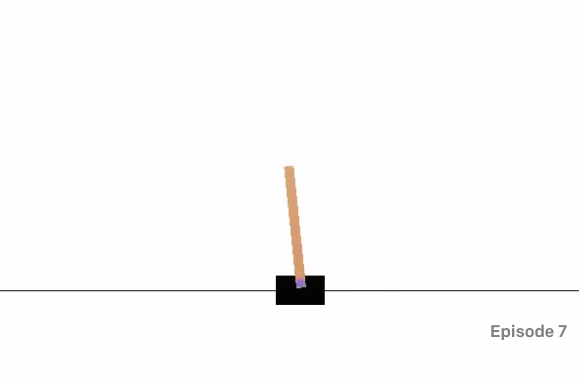
\includegraphics[height=1in]{Cartpole1.png}
    }
    \subfloat[MCC-v0]{
        \centering
        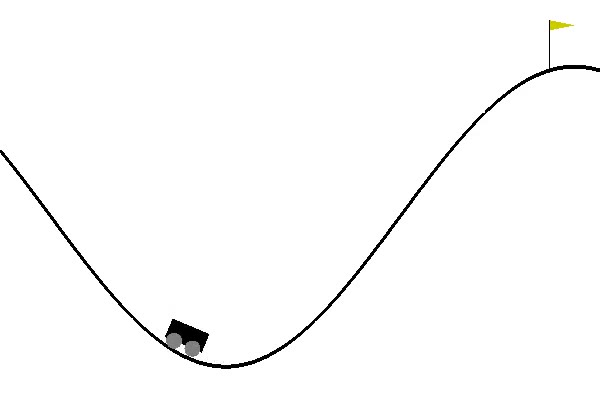
\includegraphics[height=1in]{MountainCar0.jpeg}
    }
    \subfloat[Taxi-v3]{
        \centering
        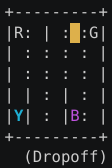
\includegraphics[height=1in]{Taxi3.png}
    }
    \subfloat[BW-v2]{
        \centering
        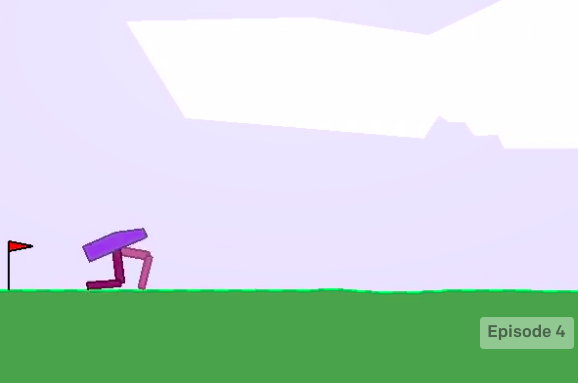
\includegraphics[height=1in]{BipedalWalker2.png}
    }
    \caption{Selected tasks}
    \label{fig:envs}
\end{figure}

We evaluate our framework on 4 low-dimensional (see section \ref{sec:summary}) POMDPs sampled from OpenAI Gym \cite{openai-gym} leaderboard\footnote{\url{https://github.com/openai/gym/wiki/Leaderboard}}:

\begin{enumerate}
\item \textbf{CartPole-v1} \cite{cartpole}.
A pole is attached to a cart.  which moves along a frictionless track.
The agent observes cart position, cart velocity, pole angle and pole velocity at tip.
The goal is to keep the pole upright by applying force between -1 and 1 to the cart.
At every step the agent receives a +1 reward for survival.
The episode terminates when the pole inclines too far.
\item MountainCarContinuous-v0 (\textbf{MCC-v0})\cite{mountain_car}.
A car is on a one-dimensional track, positioned between two "mountains". 
The goal is to drive up the mountain consuming a minimal amount of fuel by controlling the engine, setting it's torque in the range $[-1;1]$; however, the engine is not strong enough to scale the mountain in a single pass.
Therefore, the only way to succeed is to drive back and forth to build up momentum. 
We picked MountainCarContinuous-v0 as opposed to MountainCar-v0 to demonstrate the performance of our discretization system.
\item \textbf{Taxi-v3} \cite{taxi}. There are 4 locations (labeled by different letters) and the goal is to pick up the passenger at one location and drop him off in another in as few timesteps as possible spending as little fuel as possible.
\item BipedalWalker-v2 (\textbf{BW-v2}). A simulated 2D robot with legs has to learn how to walk. 
Moving rightwards is rewarded, falling is penalized.
Observation vector consists of speeds, angular speeds and joint positions collected by the robot's sensors.
These observations do not, however, include any global coordinates - they can only be inferred from sensor inputs.
With action vector of size 4 the agent controls speeds of the robots hip and knee motors.
\end{enumerate}

\paragraph{Hyperparameters}

For observation discretization (section \ref{sec:observe}) we picked $d=5$ (so that it's equal to the number of shorthands) and $h=500$ for our experiments, hence when the observation is among the highest 20\% of the last 500 observations it is written into memory as 4 while if it falls between 40-th and 60-th percentiles it is 2.

\paragraph{Expert programs}
\label{sec:expert-progs}

For \textbf{CartPole} we wrote 2 programs. 
One completely ignores all observations and just alternates between "move right" and "move left":

\begin{center}
\begin{lstlisting}
0!,1!
\end{lstlisting}
\end{center}

Another calculates the difference between velocity of the cart and angular velocity of the pole.
If it's positive, the cart is pushed to the right (the cart has to catch up with the pole), if it's negative the cart is pushed to the left, if zero it is pushed randomly:

\begin{center}
\begin{lstlisting}
[a0>0>0>0>0>@>1>1>1>1>1>,>[->>-<<]>>+++++^!1]
\end{lstlisting}
\end{center}

The first part of this program sets up an action map on the tape where every possible value of the velocity differential has a respective cell with 0, 1 or (in the center) random number.
Then \verb|[->>-<<]| block does subtraction, \verb|+++++| adds 5 to the result, so that it belongs to in $0..10$ and not $-5..5$, \verb|^| moves the memory pointer to the correct cell in the action map and \verb|!| puts the action onto the action stack.

For \textbf{Mountain Car} we wrote an elegant algorithm that reads the observation vector into the tape, goes to the second observation (car velocity) and outputs it as action:

\begin{center}
\begin{lstlisting}
>!a
\end{lstlisting}
\end{center}

In other words, we apply motor torque in the same direction where we're currently headed, thus always accelerating our car.
If we're headed right, that helps us get to the destination and if we're headed left that helps us get as high as possible onto the hill so that when direction reverses, the car has more energy to push through the right hill.

For \textbf{Taxi} we introduce 2 programs.
The first program:
\begin{enumerate}
    \item Finds the coordinates of the current destination (passenger to pick up or current passenger's destination)
    \item Subtracts the current destination 
    \item Moves in the resulting direction
\end{enumerate}

The problem with this approach is that it always gets stuck when it hits a wall.
To compensate for that, the second program alternates between the strategy above (for 5 iterations) and random movements (for 5 iterations) so that it eventually gets unstuck. See source code repository for the programs.

Optional commands \verb|@^~01234abcde| have all been invaluable in developing these programs - a fact in support of $H_4$.
A more rigorous way to confirm it would be employing several human experts to develop programs with and without optional operators, but finding volunteer \textbf{BF++} developers has proven difficult. 

Developing programs for \textbf{Bipedal Walker} is, unfortunately, above the author's paygrade. 

\paragraph{Program synthesis model}

In order to train a generative model $g$ to write \textbf{BF++} programs we treat the writing process as a reinforcement learning episode in its own right \cite{abolafiaNeuralProgramSynthesis2018} .
Every character of a program is an action taken by the \emph{writer agent}, the programs are terminated by a NULL character.
When the NULL character is written, a \emph{BF++ agent} is created in the target POMDP environment (e.g. CartPole) and sum total of rewards $Q$ collected in that episode is assigned as a reward to the \emph{writer agent} for the NULL character.
All other characters are rewarded with zero.

The \emph{writer agent's} policy is modeled with an LSTM \cite{hochreiterLongShorttermMemory1997} neural network and is trained with a modified version of REINFORCE \cite{williamsSimpleStatisticalGradientfollowing1992}algorithm.
While standard REINFORCE optimizes Policy Gradient:

\begin{equation}
    O_{\text{PG}}(\phi) = \mathbb{E_{\pi(C; \phi)}}(Q)
\end{equation}

where $\phi$ are LSTM parameters, $C$ - program, $Q$ - reward obtained by the program in target environment,

we optimize

\begin{equation}
    O(\phi)=O_{PG}(\phi)+O_{PQT}(\phi)
\end{equation}

where

\begin{equation}
    O_{\text{PQT}} = \frac{1}{K} \sum_{k=0}^K \log \pi(C_k; \phi)
\end{equation}

where $C_1$ is the best (highest $Q$) known program, $C_2$ - second best, \dots

Intuitively, both $O_{\text{PG}}(\phi)$ and $O_{\text{PQT}}(\phi)$ when optimized update the weights of the LSTM so that programs that we have found to be successful are more likely.
But Policy Gradient weighs programs proportionately to their respective rewards while PQT creates a \textit{priority queue} of the \textit{best known programs} and assigns a high importance to them and zero to the rest.

\begin{figure}
    \centering
    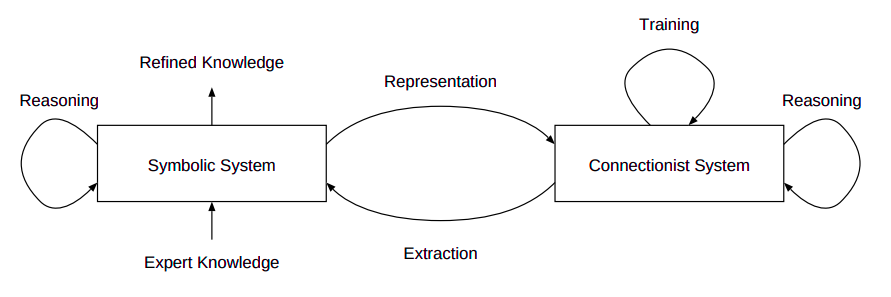
\includegraphics[width=\linewidth]{cycle.png}
    \caption{Neural-symbolic learning cycle \cite{cycle}}
    \label{fig:cycle}
\end{figure}

$O_{\text{PQT}}$ component has been shown to have "a stabilizing affect and helps reduce catastrophic forgetting in the policy" \cite{abolafiaNeuralProgramSynthesis2018}.
In addition to this, we use $O_{\text{PQT}}$ to implement \textbf{expert inspiration}.
By default, the \textit{priority queue} of the \textit{best known programs} is initialized as an empty set.
But if expert-written programs are available, it can be prepopulated with these programs that act as useful positive examples for teaching the \emph{writer agent}.
This approach is used to incorporate programs from section \ref{sec:expert-progs} and transfer knowledge from experts to the neural developer.

This approach to \textbf{expert inspiration} follows what's known as neural-symbolic learning cycle, displayed in figure \ref{fig:cycle} - expert knowledge is represented symbolically, in terms of a \textbf{BF++} program, then a neural network is trained to generate this program, effectively translating the expert knowledge from symbolic into connectionist format (\emph{representation}), the neural network learns from reinforcement how to solve the task better than the expert (\emph{training}).
Unlike in most neural-symbolic systems \cite{neuralsymbolic} that extract knowledge from connectionist systems with algortihms like TREPAN \cite{trepan} or JRip extraction \cite{jripextr}, the \emph{extraction} step is trivial since the neural network outputs a symbolic program directly.

In all experiments below, the \emph{writer agent}'s LSTM has hidden size of 50, batch size of 4 and is trained with RMSProp \cite{tielemanLectureRmsPropDivide2012} optimizer.

\paragraph{Stopping and Scoring}

All experiments were run with an upper limit of 100000 training episodes.
Environments other than \textbf{Taxi} also used Exponential Variance Elimination \cite{evestop} early stopping technique - training was stopped when the postive trend in the quality of the best found program stopped, i.e. when the exponential moving average of program quality is lower that it was 1000 episodes ago.
Agents for \textbf{Taxi} are trained for a fixed number of episodes, because we noticed that in this environment the longest part of the training process is learning to pick up your first passenger and until that happens $Q=-200$ holds.

Once the training process is finished, we take the best known programs and since each of them was only tested once (leading to high variance) we test them again, averaging total rewards over 100 episodes. 
We use this averaged reward to pick the best program.

\paragraph{Implementation}

\textbf{BF++} interpreter and the training system were written in Python with TensorFlow for neural models.
GPU resources weren't used, because the performance bottleneck of the system is not backpropagation but rather testing a \textbf{BF++} program in the environment, single experiment runtime was between 1 hour (CartPole) and 10 (Taxi).

\newpage
\section{Results}

\begin{table}[H]
  \caption{Total episode reward $Q$ achieved by best programs found, averaged over 100 episodes}
  \label{tab:quality}
  \centering
  \begin{tabular}{lcccc}
    Environment     & CartPole-v1     & MCC-v0 & Taxi-v3 & BW-v2 \\
    \midrule
    Random agent & 9.3 & 0 & -200 & -91.92  \\
    \midrule
    BF++ expert program 1 & 20.48 & -6.55 & -179.49 & - \\
    BF++ expert program 2 & 18.23 & - & -150.44 & - \\
    BF+ (without shorthands) LSTM & 44.55 & 91.57 & -57.93 & -91.9 \\
    BF+ (without \verb|@^~|) LSTM & 48.14 & 81.16 & -42.21 & -31.79 \\
    BF++ LSTM     & 71.38 & 88.41 & -199.82 & -26.97 \\
    BF++ LSTM with expert inspiration  & 96.64 & 91.39 & -60.65 & - \\
    \midrule
    Leaderboard threshold & 195 & 90 & 0 & 300 \\
    \bottomrule
  \end{tabular}
\end{table}

\paragraph{Quantitative results}

The table above presents the quality metric (average 100-episode reward) of the best program in every category, compared to that of a fully random agent and the result required to join the OpenAI gym leaderboard for context.
Note that the expert programs used a lot of optional operators (shorthands and \verb|@^!|), so it wasn't possible to implement expert inspiration with limited command sets.

These results support (see section \ref{sec:exgoals}) hypothesis $H_1$ - we have obtained functional programs for all environments, $H_2$ - when expert inspiration was used the resulting programs were better than expert programs and better than programs generated without expert inspiration and $H_4$ - ablation studies for optional operators do indeed show that those operators are useful.

\paragraph{Case studies}
\label{sec:casestudies}
% Need to make sure that this paragraph and "expert programs" paragraph help each other (same style, same terms)

We have established that the program synthesis model is able to learn from human experts.
But can experts learn from the model? ($H_3$) 
To confirm this, we offer a detailed explanation of the most successful program of all experiments listed in section \ref{sec:bfpp-experiments}.

This program scored \emph{91.39} on \textbf{Mountain Car}:

\begin{center}
\begin{lstlisting}
-..~+
\end{lstlisting}
\end{center}

The trailing \verb|~| and \verb|+| do not affect the behavior of the agent: they modify the value of the active cell only for it to be immediately rewritten by the virtual comma (section \ref{sec:virtualcomma}) before it has any chance to influence actions.
One can think about these commands as inactive genes in the DNA - we have found many resulting programs to contain such commands.
If necessary this effect can be accounted for by incorporating program length into the loss function.
So this program is equivalent to:

\begin{center}
\begin{lstlisting}
-..
\end{lstlisting}
\end{center}

\begin{figure}
    \centering
    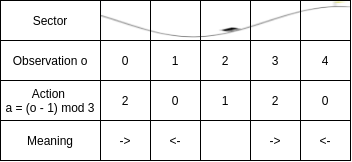
\includegraphics[width=\linewidth]{MountainCarWinner.png}
    \caption{Visual summary of the strategy enacted by \texttt{-..} on \textbf{Mountain Car}}
    \label{fig:mountaincarwinner}
\end{figure}

When the virtual comma is executed, car position and car velocity are read into memory, discretized into integers $0\dots4$.
The position is read into the active memory cell $p_T$, while the velocity is in cell $p_T+1$.
Then the active cell is decremented and the resulting number is put onto the action stack twice.
There is 1 read operation and 2 write operations to the end of the action stack, which introduces a delay before the actions get executed.
When it's time to act, the number on the action stack is coerced to one of the actions possible in this environment (0 for going left, 1 for doing nothing, 2 for right). 

A strategy emerges, illustrated on figure \ref{fig:mountaincarwinner}, in which the car puts "going right" onto the agenda if it's on the far left or the center right of the landscape, puts "going left" onto the agenda when it's on the far right or center left and schedules doing nothing if it's in the center.
This strategy helps the car successfully reach the right fringe every time it is applied.

\newpage
\section{Conclusions}

In this chapter, we have introduced a new programming language tailored to the task of programmatically interpretable reinforcement learning.
We have shown experimentally that this language can facilitate program synthesis as well as knowledge transfer between expert-based systems and data-driven systems. 

The results in the OpenAI gym test examples show that the proposed system is able to find a functional solution to the problem. In some cases the performance is similar to the best deep learning solution but the obtained program remains still explainable. This is a very encouraging result and suggest that the use of program induction methods may indeed be a viable way towards explainable solutions in RL applications. 

We propose the following directions for future work:
\begin{enumerate}
    \item Develop translation mechanisms between \textbf{BF++} and other languages. Potentially, \textbf{BF++} can be used as \emph{bytecode} \cite{bytecode} for reinforcement learning. The expert would write a program in a higher-level language and transpile it into \textbf{BF++} so that the program then can be improved with reinforcement learning.
    \item Use other neural network architectures as well as non-neural evolution methods like genetic programming \cite{genprog1,genprog2} in conjunction with \textbf{BF++}
    \item Apply the framework to problems in Healthcare where expert inspiration is important for crossing the AI chasm \cite{aichasm}.    \item Use Natural Language Generation techniques to translate the BF++ code automatically to a friendly human-readable text description as in \cite{richardsonCode2TextChallengeText2017,code2nlg2}.
\end{enumerate}

\newpage
\chapter{A Neurogenetic Programming Framework}
\epigraph{}{}

\section{Introduction}\label{sec:intro}

Automatic programming is a discipline that studies application of mathematical models to infer programs from data and use these generated programs to solve various tasks.
For example, given a dataset of clinical decision-making generate a program that describes how doctors make treatment decisions based on clinical history available to them.

One of the primary motivations behind automatic programming is enabling an exchange of knowledge between human experts and machine learning models: black box models have achieved impressive results in diverse decision support settings \cite{deeprl}, sometimes competing with human experts in the field. The advantage of automatic programming systems is that they can also \emph{cooperate} with the experts:
\begin{itemize}
    \item Code generation models can be trained to produce programs similar to what experts wrote, incorporating expert knowledge into the model
    \item Code generation models can generate new programs by applying modifications to expert-written programs, using them as the basis
    \item Experts can examine the generated programs, understand the algorithm suggested by the system and learn from it
\end{itemize}

% Vadim: just some brain dumping for an intro candidate
The benefits of regulating the program induction task, especially in limited data conditions have been demonstrated earlier \cite{metainduction}. The programming language used in program induction is a regulating constraint that may be expected to guide the learning algorithm to favor solutions with operations that are most natural for the given language \cite{massiveparallelism}. For example, a strictly sequential language such as C seems most natural in cases where the expected solution is a sequential protocol. A parallel language, such as various cellular automata models or deep neural networks, favor concurrent solutions. 

We may also approach this from the angle of algorithmic information theory. The Kolmogorov complexity of the solution corresponds to the length of the program and the number of free parameters \cite{kolmogorov}. In the case of a black box deep model, the Kolmogorov complexity is an architectural constant of the parallel network model while in program induction it is optimized by the learning algorithm based on the available training data. When data is limited, the PI training may use {\sl Occam's razor  \footnote{"We consider it a good principle to explain the phenomena by the simplest hypothesis possible" \cite[book 3, chapter 2]{ptolemy}, misattributed \cite{occam} to William of Ockham }} to find a minimal-complexity solution matching the training data, while a standard NN solution always has the same complexity. 

In fact, the use of program synthesis for solving a machine learning problem can be seen as {\sl generalized hyperparameter optimization}; the program optimization may, in principle, converge to a program that implements a particular deep neural network optimized for the problem. 
% or is this philosophical bullshit going too far for your taste already ;)
%AH: added last paragraph by reprogramming later text
 In \emph{genetic programming} \cite{genprog,genprogast} new programs are generated by mutating and mixing a \emph{population} of programs. 
 A more recent approach, largely drawing on the earlier success of deep neural language models (see CodeBERT \cite{codebert} inspired by BERT \cite{devlinBERTPretrainingDeep2019}), have been to train black box \emph{neural models} that generate executable programs as text \cite{brain-coder,deepcoder,structural}. 
 Neural program synthesis and genetic programming both have unique advantages \cite{geneticvsneural}. 
 In this chapter we propose a novel hybrid of the two families of methods. We call the method \emph{Instant Scrum} in reference to a popular Agile software team work model \cite{scrum}. We show that \emph{Instant Scrum}, IS, can solve several reinforcement-guided program synthesis tasks in standard OpenAI gym benchmarks tasks (section \ref{sec:tasks}). 

After the introduction to the relevant background in the next section, we will give a detailed description of the proposed IS methodology. Next, we describe the experimental setup and the OpenAI gym test tasks, and the results of the experiments in several variations of the core IS method. Finally, we discuss the results and propose future research directions and potential applications for hybrid neurogenetic programming. 

% TODO: Evolutionary strategies in RL

\newpage
\section{Background}

% TODO: Review solutions, not just problems

\emph{Specification} is central to the field of automatic programming: if no requirements to generated programs are specified, the task becomes random program generation - not useful in most real-world settings beyond testing compilers \cite{random1,random2}.
The field of automatic programming can be subdivided by what type of specification is used.

One way to specify expected behavior of a program is a dataset of input-output pairs \cite{deepcoder,brain-coder}.
A lot of work in this area has been inspired \cite{flashmeta,flash1,flash2} by the task of learning a formula that fits a series of cells in spreadsheet applications \cite{flashfill}.

Alternatively, the program's pre- and postcondition predicates can be described in a formal language: \emph{proof-theoretic synthesis} \cite{prooftheoretic} is the task of generating a program such that if it's input conforms to the precondition, its output has to conform to the postcondition.

In the task of \emph{semantic parsing} \cite{hearthstone,semparsing1,rabinovich2017abstract}, specification is a textual description of an algorithm that has to be translated from  natural language into machine language.

Finally, specification can manifest in the form of a \emph{reinforcement learning environment} \cite{pirl} - a program defines behavior of an agent that interacts with its environments and receives positive and negative rewards from it.
The goal is to find a program that maximises rewards.
In this work, we choose RL specification, because it generalizes other methods: input-output pairs can be seen as an environment that negatively reinforces a metric of difference between expected and observed program output, while in \emph{proof-theoretic synthesis} the reward is determined by the postcondition.  
Many real-world problems, such as robot control \cite{robotrl} and clinical decision making \cite{heartpole,gym-sepsis} are formulated as reinforcement learning as well.

\newpage \subsection{Programmatically Interpretable Reinforcement Learning}
\label{sec:pirl}

More concretely, we model the task as {\em Episodic Partially Observable Markov Decision Process}:

\begin{multline}
M = (\mathcal{S}_{nt}, \mathcal{S}_t, \mathcal{A}, \mathcal{O}, p_o(o | s, a), p_s(s_\text{next} | s_\text{prev}), p_r(r | s, a), p_\text{init}(s))
\end{multline}

Here, $\mathcal{S}_{nt}$ is the set of {\em non-terminal (environment) states} and $\mathcal{S}_{t}$ is the set of {\em terminal states}. 
$\mathcal{A}$ is the set of {\em actions} that the learning agent can perform, and $\mathcal{O}$ is the set of {\em observations} about the current state that the agent can make. 

A \emph{reinforcement learning episode} starts in a state $s \in \mathcal{S}_{nt}$ sampled from $p_\text{init}$, the {\em initial distribution} over environment states.
An agent action $a \in \mathcal{A}$ at the state $s$ causes the environment state to change probabilistically, and the destination state follows the distribution $p_s(\cdot | s, a)$. 
At state $s$, the probability of making observation $o$ is $p_o(o | s)$ and the probability of obtaining \emph{reward} $r$ is $p_r(r|s,a)$. 
The process continues until a $p_s$ yields a terminal state $s \in \mathcal{S}_t$.
This distinction is what sets \emph{episodic} POMDP popularized by OpenAI gym \cite{gym} apart from the more traditional approach \cite{pomdp1,pomdp2} where the process is infinite.

A \emph{program} is a sequence of tokens

\begin{equation}
    c=(c^{(1)},c^{(2)},\dots)
\end{equation}

that defines behavior of an agent.
Depending on the programming language and implementation choices the tokens can be characters or higher-level tokens, i.e. keywords.
We denote the language's \emph{alphabet}, i.e. the set of all possible tokens as $\mathcal{L}$.

An \emph{interpreter} is a tuple $\langle \alpha,\mu \rangle$ where $\mu(c_k,m_k,o_k)$ is the \emph{memorization function} that defines how the agent's memory updates upon making an observation and $\alpha(c, m_k)$ is the \emph{action function} defines which action the agent at a certain memory state takes in the POMDP.
Memory is intialized at state $m_\text{init}$

The agent's goal is maximizing total reward collected in the environment, calculated as follows:

\begin{algorithm}[H]
\begin{algorithmic}[1]
\caption{Evaluating total reward for a program}
\Function{$\mathit{Eval}$}{$c$}
\State $R_\text{tot} \gets 0$
\State $m \gets m_\text{init}$
\State $s \sim p_\text{init}(s)$
\While{$s \in \mathcal{S}_{nt}$}
\State $o \sim p_o(o | s)$
\Comment{Observe}
\State $m \gets \mu(c,m,o)$
\State $a \gets \alpha(c, m)$ 
\Comment{Act}
\State $r \sim p_r(s,a)$
\State $R_\text{tot} \gets R_\text{tot} + r$
\Comment{Get rewarded}
\State $s_\text{next} \sim p_s(s_\text{next} | s, a)$
\Comment{Next state}
\State $s\gets s_\text{next}$
\EndWhile
\State \Return $R_\text{tot}$
\EndFunction
\end{algorithmic}
\end{algorithm}

Since the algorithm for computing this function involves repeatedly sampling values from distributions, function $\mathit{Eval}(c)$ is a mapping from the set of programs to the set of real-valued random variables.

\emph{Programmatically Interpretable Reinforcement Learning} \cite{pirl} is the task of maximizing expected total reward with respect to $c$, i.e. finding a program $c$ that is best for a given POMDP environment:

\begin{equation}
    \mathbb{E}(\mathit{Eval}(c)) \longrightarrow \max_{c}
    \label{eq:pirlgoal}
\end{equation}

\newpage
\section{Methodology}
\label{sec:methodology}

How does one manage a composition of code generators in such a way that the composition yields better programs than individual contributors are capable of? 
This question is studied extensively in software project management literature \cite{mythicalmanmonth}.
And while, admittedly, project management literature is concerned with human developers and, admittedly, there exist considerable differences between human developers and mathematical models of code generation \cite{bugfixing}, we mitigate these differences with several simplifying assumptions.

\newpage \subsection{Modeling the codebase}

Following from traditional genetic programming, we define a \emph{population} of programs. 
The \emph{codebase} is a tuple of 2-tuples, representing a program $C_c^{(i)}=c$ and the total reward it collected $C_R^{(i)}=R_\text{tot} \sim \mathit{Eval}(c)$ (see section \ref{sec:quality}):

\begin{equation}
    \mathcal{C} = \langle \langle C_c^{(1)}, C_R^{(1)} \rangle, \langle C_c^{(2)}, C_R^{(2)} \rangle \dots \langle C_c^{(|C|)}, C_R^{(|C|)} \rangle \rangle
\end{equation}

However, unlike in traditional genetic programming, the \emph{initial population} can (optionally) be empty.

\newpage \subsection{Modeling a software developer}
\label{sec:developer}

A software developer can:
\begin{enumerate}
    \item Check out programs from the codebase $\mathcal{C}$
    \item Output new a program $c$
    \item Receive feedback on their program's quality $q$ 
    \item Learn from the feedback by mofidying its strategy
\end{enumerate}

Thus, a developer is a 2-tuple of a program distribution $p_\text{dev}(c | \theta, \mathcal{C})$ and a parameter update procedure $\mathit{Update}(\theta, c, q)$

Distribution $p_{\text{dev}}(c | \theta, \mathcal{C})$ is defined over programs and is parametrized with learnable parameters $\theta$ as well as codebase $\mathcal{C}$. 
Having codebase as parameter enables the developer to generate new programs as a modification and/or combination of existing programs, i.e. to apply genetic programming.

Learnable parameters $\theta$ encode the developer's current methodology of programming that can be modified upon receipt of positive or negative feedback using the developer's update procedure. 

The \emph{team} of developers is a tuple of 2-tuples:
\begin{equation}
    \mathcal{T} = \langle \langle \mathcal{T}_p^{(1)}, \mathcal{T}_\text{upd}^{(1)} \rangle, \langle \mathcal{T}_p^{(2)}, \mathcal{T}_\text{upd}^{(2)} \rangle \dots \langle \mathcal{T}_p^{(|\mathcal{T}|)}, \mathcal{T}_\text{upd}^{(|\mathcal{T}|)} \rangle \rangle
\end{equation}

\newpage \subsection{Modeling program quality}
\label{sec:quality}

We define two empirical metrics of overall program fitness.
The first is \emph{empirical total reward}:

\begin{equation}
    R(c|\mathcal{C}) = \frac{\sum\limits_{i=1}^{|C|} \mathbb{I}[C_c^{(i)}=c] C_R^{(i)}}{\sum\limits_{i=1}^{|C|} \mathbb{I}[C_c^{(i)}=c]}
\end{equation}

If a program has been tested in the environment ($\textit{Eval()}$ function) several times, there will be several copies of it in the codebase with different quality samples.
Averaging over them yields an unbiased estimate of the expectation from equation \ref{eq:pirlgoal}, $\mathbb{E}(\mathit{Eval}(c))$, that we set out to maximize.

The second is \emph{empirical program quality}, defined as

\begin{equation}
    Q(c|\mathcal{C}) = \frac{\sum\limits_{i=1}^{|C|} \mathbb{I}[C_c^{(i)}=c] e^{C_R^{(i)}}}{\sum\limits_{i=1}^{|C|} \mathbb{I}[C_c^{(i)}=c]}
    \label{eq:empquality}
\end{equation}

\emph{Empirical program quality} is an unbiased estimate of $\mathbb{E}(e^{\mathit{Eval}(c)})$
The idea behind exponentiating the total reward is to encourage \emph{exploration} \cite{exploration}.
Programs that on average perform poorly, but sometimes, stochastically, collect high rewards, will have a higher $Q(c|C)$ than $R(c|C)$.
We consider these programs to be \emph{high-quality additions to the codebase} because they contain the knowledge necessary for solving environment $M$, even if on average they don't solve it.
We hypothesize that applying \emph{genetic operators} (section \ref{sec:genetic}) to programs with high $Q(c|C)$ can yield programs with high $R(c|C)$.
For this reason we train developers to maximize $Q$, but when the training is complete, we pick programs from the codebase with the highest $R$ as "best programs".
 
$Q(c|C)$ has an additional technical advantage over $R(c|C)$: invariant $Q(c|C) \geq 0$ holds for all $c$.
This lets one sample programs from the codebase with probabilities proportional to their quality, see eq. \ref{eq:genmixture}.

\newpage \subsection{Populating the codebase}

Just like \emph{instant run-off voting} achieves similar results to \emph{exhaustive ballot runoff voting}, but does it much faster by replacing a series of ballots cast in a series of elections with a ballot cast once that goes on to participate in a series of virtual elections \cite{votingsystems}, our \emph{Instant Scrum} algorithm does the same to Scrum \cite{scrum}: it simulates the iterative software development process recommended by Scrum methodology without humans in the loop making it possible to run many sprints per second:

\begin{algorithm}[H]
\begin{algorithmic}[1]
\caption{Instant Scrum with a team of developers}
\label{alg:instantscrum}
\Procedure{InstantScrum}{$T,\mathcal{C},N_\text{max}$}
\State $N \gets 0$
\While{$N < N_\text{max}$}
\LineComment{For each developer in the team}
\For{$i = 1,2,\dots,|T|$}
\LineComment{Sample a program from the developer}
\State $c_\text{new}\sim p_i(c | \theta_i, \mathcal{C})$ 
\LineComment{Test the program}
\State $R_\text{tot} \gets \mathit{Eval}(c_\text{new})$
\LineComment{Save the code and test result to the codebase}
\State $\mathcal{C} \gets \mathcal{C} \cup \{\langle c_\text{new}, R_\text{tot} \rangle\}$
\LineComment{Train the developer}
\State $\mathit{Update}_i(\theta_i, c, q)$
\LineComment{Increment sprint counter}
\State $N \gets N+1$
\EndFor
\EndWhile
\EndProcedure
\end{algorithmic}
\end{algorithm}

To combine genetic programming and neural program synthesis we introduce 3 types of developers: \emph{genetic} and \emph{neural} and \emph{dummy}, create a team that contains developers of all types and run \emph{Instant Scrum}.

\newpage \subsection{Genetic developers}
\label{sec:genetic}

A genetic developer writes programs by
\begin{enumerate}
    \item Selecting one of the 7 available stochastic \emph{genetic operators} (described below)
    \item Selecting two programs from the \emph{codebase} $C$ (parents $c_1$ and $c_2$) 
    \item Using the operator to modify the parents and yield a new (child) program
\end{enumerate}

A genetic operator is a probability distribution $p_\text{op}$ over child programs given 2 parent programs. 

\begin{equation}
    p_\text{op}(c_\text{child}|c_1,c_2)
\end{equation}

Operators whose $p_\text{op}$ is invariant to $c_2$ and depends on $c_1$ only are called \emph{mutation} operators: they generate a new program by \emph{mutating} one program $c_1$.
The rest are called \emph{combination} operators as they \emph{combine} 2 existing programs to generate a new one.



\paragraph{Mutation operators}

The simplest method for randomly modifying a program is \emph{shuffle mutation}: randomly re-order the tokens of $c_1$.
Let $\mathrm{A}$ be the set of all possible permutations of size $|c_1|$. $|\mathrm{A}|=|c_1|!$. 
Then

\begin{equation}
    p_\text{shuffle}(c_\text{child}|c_1,c_2) =
            \frac{\sum\limits_{\alpha \in \mathrm{A}} \mathbb{I}[\alpha(c_\text{parent}) = c_\text{child}]}{|c_1|!}
\end{equation}

Another approach is \emph{uniform mutation} where a loaded coin is tossed for every token in $c_1$. 
With probability $p_\text{ind}$ it is replaced with a random token from the alphabet $\mathcal{L}$ of the programming language, with probability $1-p_\text{ind}$ it stays the same.
The evolution of a single token under shuffle mutation is defined by distribution

\begin{equation}
    p(c^\text{new} | c^\text{old}) = \frac{p_\text{ind}}{|L|} +  (1 - p_\text{ind}) \mathbb{I}[c^\text{new} = c^\text{old}]
\end{equation}

Hence over full programs the operator is defined as

\begin{equation}
    p_\text{unimut}(c_\text{child}|c_1,c_2) = \mathbb{I}[|c_\text{child}|=|c_1|] \\ 
    \prod\limits_{i=0}^{|c_1|}  \left(\frac{p_\text{ind}}{|L|} +  (1 - p_\text{ind}) \mathbb{I}[c_\text{child}^{(i)} = c_1^{(i)}] \right)
\end{equation}

\paragraph{Combination operators}

The combination operators we propose are all variants of \emph{crossover} - a classic genetic programming technique rooted in the way a pair of DNA molecules exchanges genes during mitosis and meiosis, displayed on figure \ref{fig:crossover}.

In DNA \cite{evocritique}, as well as in most genetic programming literature \cite{genprog,genprogast} the crossover operator combines 2 parent sequences to produce 2 children.
In this section, in order to reduce complexity, we define the distributions as if only the first child program is saved and the second one is forgotten.
Since program pair $\langle c_2, c_1 \rangle$ is equally likely to be selected for combination as $\langle c_1, c_2 \rangle$ (see eq. \ref{eq:genmixture}) this modification does not affect the resulting genetic developer distribution.

In \emph{one-point crossover} a random cut position $k$ is selected and the trailing sections of 2 parent programs beginning with the cut point are swapped with each other. 
If the parent programs have different lengths, the cut point has to fit within both programs:

\begin{equation}
    2 \leq k \leq |c_1,c_2|; |c_1,c_2| = \min\{|c_1|, |c_2|\}
\end{equation}

Hence the probability of $c_\text{child}$ being born out of \emph{one-point crossover} is

\begin{equation}
    p_\text{1ptcx}(c_\text{child}|c_1,c_2) =
        \frac{\mathbb{I}[|c_\text{child}|=|c_2|]}{|c_1,c_2|-1}
        \sum\limits_{k=2}^{|c_1,c_2|} \prod\limits_{i=1}^{k-1} \mathbb{I}[c_\text{child}^{(i)} = c_1^{(i)}] \prod\limits_{i=k}^{|c_2|} \mathbb{I}[c_\text{child}^{(i)} = c_2^{(i)}]
\end{equation}

\emph{Two-point crossover} is similar, but instead of swapping the trailing ends of programs, a section in the middle of the programs is chosen, determined by randomly selected cut-off indices $k_1$ and $k_2$ and swapped:

\begin{equation}
\begin{split}
    p_\text{2ptcx}(c_\text{child}|c_1,c_2) = // =
        \frac{2 \mathbb{I}[|c_\text{child}|=|c_1|]}{(|c_1,c_2|-2)(|c_1,c_2|-1)}
        \sum\limits_{k_1=2}^{|c_1,c_2|-1}
        \sum\limits_{k_2=k_1+1}^{|c_1,c_2|} \\
        \prod\limits_{i=1}^{k_1-1} \mathbb{I}[c_\text{child}^{(i)} = c_1^{(i)}] \prod\limits_{i=k_1}^{k_2-1} \mathbb{I}[c_\text{child}^{(i)} = c_2^{(i)}]
        \prod\limits_{i=k_2}^{|c_1|} \mathbb{I}[c_\text{child}^{(i)} = c_1^{(i)}]
\end{split}
\end{equation}

\emph{Uniform crossover} mirrors \emph{uniform mutation} in that a loaded coin is tossed for each token in $c_1$. With probability $p_\text{ind}$ the token is replaced, but the replacement is not drawn randomly from the alphabet. Instead, the replacement comes from $c_2$:

\begin{equation}
    p_\text{unicx}(c_\text{child}|c_1,c_2) = \prod\limits_{i=0}^{|c_1|} \mathbb{I}[|c_\text{child}|=|c_1|] \\ \left(p_\text{ind} \mathbb{I}[c_\text{child}^{(i)} = c_2^{(i)}] + (1 - p_\text{ind}) \mathbb{I}[c_\text{child}^{(i)} = c_1^{(i)}] \right)
\end{equation}

Finally, \emph{messy crossover} is a version of \emph{one-point crossover} without the assumption that both parent programs have to be cut at the same index $k$.
In \emph{messy crossover}, one parent is cut at index $k_1$, another is cut at index $k_2$ and the head of one is attached to the tail of the other:

\begin{equation}
    p_\text{messy}(c_\text{child}|c_1,c_2) =
        \frac{1}{(|c_1,c_2|-1)^2}
        \sum\limits_{k_1=2}^{|c_1,c_2|} \sum\limits_{k_2=2}^{|c_1,c_2|} \\ \mathbb{I}[|c_\text{child}|=k_1+|c_2|-k_2] \\ \prod\limits_{i=1}^{k_1-1} \mathbb{I}[c_\text{child}^{(i)} = c_1^{(i)}] \prod\limits_{i=1}^{|c_2|-k_2} \mathbb{I}[c_\text{child}^{(k_1+i)} = c_2^{(k_2+i)}]
\end{equation}

\begin{figure}
    \centering
    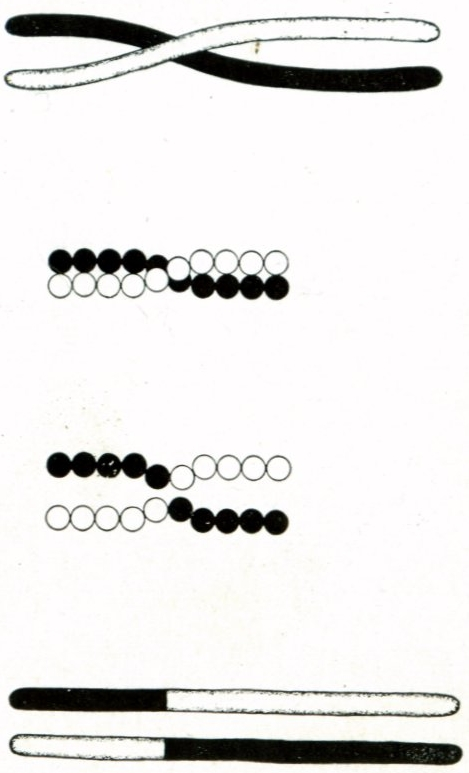
\includegraphics[width=0.45\linewidth]{Morgan_crossover_1.jpg}
    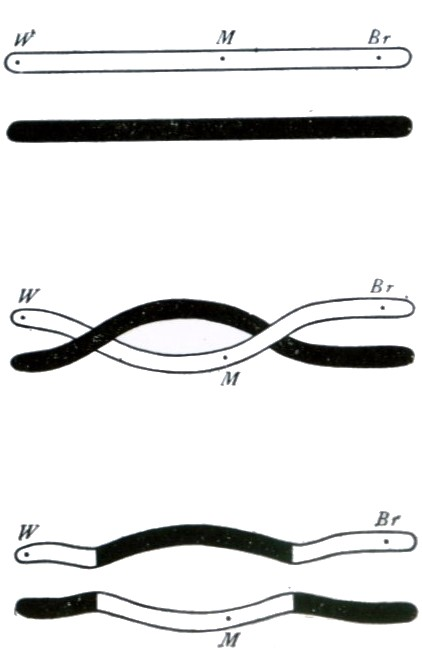
\includegraphics[width=0.5\linewidth]{Morgan_crossover_2.jpg}
    \caption{1-point and 2-point crossover \cite{evocritique}}
    \label{fig:crossover}
\end{figure}

\begin{table}
    \centering
    \begin{tabular}{r|l}
         Parent 1 & \color{blue}\verb|ae>>>>>34+| \\
         Parent 2 & \color{red}\verb|a[e>-a-]b[e>>-b-]| \\
         \midrule
         Shuffle mutation & \color{blue}\verb|>>4+>3>e>a| \\
         Uniform mutation & \color{blue}\verb|ae|\color{black}\verb|@|\color{blue}\verb|>|\color{black}\verb|!|\color{blue}\verb|>>3|\color{black}\verb|5|\color{blue}\verb|+| \\
         1-point crossover & \color{blue}\verb|ae>>>>|\color{red}\verb|-]b[e>>-b-]| \\
         2-point crossover & \color{blue}\verb|ae>|\color{red}\verb|>-a-|\color{blue}\verb|34+| \\
         Uniform crossover & \color{blue}\verb|ae|\color{red}\verb|e|\color{blue}\verb|>|\color{red}\verb|-|\color{blue}\verb|>>3|\color{red}\verb|b|\color{blue}\verb|+| \\
         Messy crossover & \color{blue}\verb|ae>>>>|\color{red}\verb|e>-a-]b[e>>-b-]| \\
         Pruning & \color{blue}\verb|e>>>>>4+| \\
    \end{tabular}
    \caption{All operators applied a pair of BF++ \cite{bf++} programs}
\end{table}


\paragraph{Pruning operator}

After initial experiments  we found that generated programs often contain sections of unreachable code or code that makes changes to the execution state and fully reverses them.
To address this, we introduced an additional operator for removing dead code (\emph{pruning}): when Instant Scrum encounters a successful program, pruning helps separate sections of this program that led to its success from sections that appeared in a highly-rated program by accident.  

Implementation of the pruning operator depends on the programming language at hand, here we define it as a pruning function $c_\text{pruned}=\mathit{Prune}(c_1)$ that outputs a program functionally equivalent to $c_1$ (memory functions $(\alpha,\mu)$ of $c_\text{pruned}$ are equal to that of $c_1$) and $|c_\text{pruned}| \leq c_1$ and a degenerate probability distribution:

\begin{equation}
    p_\text{prune}(c_\text{child}|c_1,c_2)= \begin{cases}
        1 & c_\text{child} = \mathit{Prune}(c_1) \\
        0 & \text{otherwise}
        \end{cases}
\end{equation}

\paragraph{Operator and parent selection}
\label{sec:selection}

Let $\mathcal{P}_\text{genetic}$ be a tuple of all available genetic operators, in order of introduction, i.e. $\mathcal{P}_\text{genetic}^{(1)}=p_\text{shuffle}$ and $\mathcal{P}_\text{genetic}^{(4)}=p_\text{2ptcx}$

Genetic developer's program distribution is a mixture distribution, combining different operators that can be applied, weighted by learnable parameters, and different programs that can be sampled from the codebase, weighted by \emph{empirical quality} (eq. \ref{eq:empquality}).

\begin{equation}
    p_\text{genetic}(c | \theta, \mathcal{C}) = 
    \sum\limits_{c_1}^{C}  
    \sum\limits_{c_2}^{C} 
    \frac{Q(c_1|C) Q(c_2|C)}{(\sum\limits_{c}^{C} Q(c|C))^2} 
    \sum\limits_{i=0}^{|\mathcal{P}_\text{genetic}|} 
    \theta_i \mathcal{P}_\text{genetic}^{(i)} (c|c_1,c_2)
    \label{eq:genmixture}
\end{equation}

This is a true probability distribution if and only if $\sum\limits_{i=0}^{|\mathcal{P}_\text{genetic}|} 
    \theta_i = 1$


\paragraph{Training the genetic developer}

One challenge that remains to be solved to fully define the genetic developer (folowing section \ref{sec:developer}) is to define a learning from feedback strategy $\mathit{Update}_\text{genetic}$.
To do this, we notice that equation \ref{eq:genmixture} contains a \emph{multi-armed bandit} \cite{banditproblem} hiding in plain sight.
Indeed, once the \emph{genetic} developer samples $c_1$ and $c_2$ from the codebase, it has to pick one of 7 available options (pull one of 7 \emph{levers}) to then receive a reward $\mathit{Eval}(c_\text{child})$.
This subproblem can be represented with a POMDP of its own and solved using one of the standard bandit algorithms \cite{banditsolutions}.

Following \emph{Occam's razor}, we picked the simplest method, \emph{epsilon-greedy optimization}: we calculate the value of each operator as mean total reward of programs generated with this operator:

\begin{equation}
    V^{(i)} = \frac{1}{|\mathcal{C}(\mathcal{P}_\text{genetic}^{(i)})|} 
    \sum\limits_{k=1}^{|\mathcal{C}(\mathcal{P}_\text{genetic}^{(i)})|}
    \mathcal{C}(\mathcal{P}_\text{genetic}^{(i)})_R^{(k)} 
\end{equation}

where $C(\mathcal{P}_\text{genetic}^{(i)})$ is the subset of the codebase produced via operator $\mathcal{P}_\text{genetic}^{(i)}$.

The $\mathit{Update}_\text{genetic}$ procedure recalculates values $V$ and sets operator probabilities to

\begin{equation}
    \theta_i = \frac{\epsilon}{|\mathcal{P}_\text{genetic}^{(i)}|} +
    \mathbb{I}[i = \underset{i}{\arg\max} V^{(i)}] (1 - \epsilon)
\end{equation}

where $\epsilon$ is a hyperparameter responsible for regulating the \emph{exploration-exploitation tradeoff} \cite{banditsexplo}

In future work, however, other bandit optimization algorithms can be used in its place \footnote{Our open-source software implementation allows for drop-in replacement of bandit algorithms}.

\paragraph{Hyperparameters}
\label{sec:genhyper}

The genetic developer, as described above, has 2 hyperparameters:

\begin{enumerate}
    \item $p_\text{ind}$ defines severity of mutation in $p_\text{unimut}$ and $p_\text{unicx}$
    \item $\epsilon$ defines learnability of genetic operator distribution
\end{enumerate}

Note that the \emph{team} mechanism afforded by \emph{Instant Scrum} can be used not only to combine genetic and neural program synthesis, but also to combine several genetic developers with different hyperparameters.

\newpage \subsection{Neural developers}
\label{sec:neural}

The \emph{neural developer}, also known as the \emph{senior developer} because of their unique ability to write original programs, is an LSTM \cite{hochreiterLongShorttermMemory1997} network followed by a linear layer that generates a sequence of vectors $h_{1},h_{2},h_{3},\dots$ where $h_i \in \mathbb{R}^{|\mathcal{L}| + 1} \forall i$ and $j$-th element of vector $h_i$, $h_i^{(j)}$, represents the probability of $i$-th token of the program being $j$-th token in the alphabet, $p(c^{(i)}=\mathcal{L}^{(j)})$.
The last element of the vector represents a special \emph{end of program} symbol.
This vector depends deterministically on the full set of neural network parameters (LSTM and linear layer) $\theta$ and can be represented as a function $h_i(\theta)$.
Then

\begin{equation}
    p_\text{neural}(c | \theta, \mathcal{C}) = h_{(|c|+1)}^{\mathcal{L}+1}
    \prod\limits_{i=1}^{|c|}
    \sum\limits_{j=1}^{|\mathcal{L}|} \mathbb{I}[c^{(i)}=\mathcal{L}^{(j)}]
    h_i(\theta)
\end{equation}

For the $\mathit{Update}_\text{neural}$ procedure we use the algorithm proposed in \cite{brain-coder}.
The subproblem of generating a program $c$ is considered as a reinforcement learning episode of it's own, where tokens are actions and token number $|c|+1$ (\emph{end of program} token) is assigned reward $q = e^R; R \sim Eval(c)$. 
In this subenvironment $h_i(\theta)$ is the policy network \cite[chapter 13]{suttonReinforcementLearningSecond2018} trained using REINFORCE algorithm with Priority Queue Training.
This algorithm involves a priority queue of best known programs: we implement it as programs from $C$ with highest $Q(c|C)$ which means that the neural developer can train on programs written by other developers.

$h_i(\theta)$ can also represent several LSTM layers stacked or a different type of recurrent neural network, i.e. GRU \cite{gru}.
Hyperparameters of this neural network, such as hidden state size and/or number of stacked layers are hyperparameters of the neural developer.  

\newpage \subsection{Dummy developer}

The last developer we introduce is the simplest one:

\begin{equation}
    p_\text{dummy}(c_\text{child}|c_1,c_2) = 
    \frac{Q(c_\text{child}|C)}{\sum\limits_{c}^{C} Q(c|C)} 
    \label{eq:dummy}
\end{equation}

Dummy developer does not generate novel programs.
Instead, it uses the same quality-weighted program sampling as in equation \ref{eq:genmixture} to decide which existing program to copy.
Their utility may not be obvious at first, but note (section \ref{sec:quality}) that when the same program is added to the codebase several times, it's total reward and quality estimates are averaged and grow more accurate.

Dummy developer is a smart compromise between speed at which \emph{Instant Scrum} (algorithm \ref{alg:instantscrum}) is searching the program space and the quality of its working map of the program space, focusing on its most "interesting" (high $Q(c|C)$) parts. 
Without dummy developer, all empirical total rewards $E[Eval(c)]$ would be low quality estimates of true fitness of the program and one spurious success of an otherwise bad program could steer the search in the wrong direction.
On the other hand, we could test each program many times before adding it to the codebase, but that would slow down the search prohibitively. 

\newpage
\section{Experimental setup}
\label{sec:experiments}

\paragraph{Teams}

In the table below, we introduce 5 teams.
Neural developers are denoted as lstm(hidden state dimensionality), several numbers mean a stacked LSTM.
Genetic developers are denoted as $\text{gen}(p_\text{ind},\epsilon)$, see secion \ref{sec:genhyper}.
$T_\text{small}$ and $T_\text{large}$ are recommended configurations while $T_\text{genetic}$, $T_\text{neural}$ are \emph{ablation studies} to prove that combination of neural and genetic methods is useful.

\begin{table}[H]
\centering
\begin{tabular}{r|c|c|c|c}
     Developer & $T_\text{small}$ & $T_\text{large}$ & $T_\text{genetic}$ & $T_\text{neural}$  \\
     $\text{lstm}(10)$ & & \checkmark & & \\
     $\text{lstm}(50)$ & & \checkmark & & \\
     $\text{lstm}(256)$ & & \checkmark & & \\
     $\text{lstm}(10,10)$ & & \checkmark & & \\
     $\text{lstm}(50,50)$ & \checkmark & \checkmark & & \checkmark \\
     $\text{lstm}(256,256)$ & & \checkmark & & \\
     $\text{gen}(0.2,0.2)$ & \checkmark & &  & \\
     $\text{gen}(\frac{1}{3},0.2)$ & & \checkmark & & \\
     $\text{gen}(\frac{1}{6},0.2)$ & & \checkmark & & \\
     $\text{gen}(\frac{1}{12},0.2)$ & & \checkmark & & \\
     dummy & \checkmark & \checkmark & \checkmark & \checkmark \\
\end{tabular}
\caption{Team composition}
\end{table}


\paragraph{Language}

Instant Scrum can be used to generate programs in any programming language provided:
\begin{enumerate}
    \item An interpreter $\langle \alpha,\mu \rangle$, see section \ref{sec:pirl}
    \item A known finite alphabet $\mathcal{L}$
    \item A pruning function $\mathit{Prune}(c)$
\end{enumerate}

%Moreover, pruning function and finite alphabet are, in a sense, optional requirements: pruning isn't essential to the method, so a dummy pruning function $P(c)=c$ can be used instead and if a language's alphabet is infinite, it is usually possible to develop a reasonable finite subset of the full alphabet and generate programs in it.

% Ode to BF++

% A word on trees
The complexity of the chosen language is important since in complex languages random perturbations of program source code often produce grammatically invalid programs.
This issue has been addressed with \emph{structural models} \cite{grammargp,structural} \cite[chapter 4]{genprogast}, however, we sidestep the issue entirely by using \emph{BF++} \cite{bf++} - a simple language developed for \emph{programmatically interpretable reinforcement learning} where most random combinations of characters are valid programs.
Each BF++ command is represented with a single character, thus the only way to tokenize it is to let tokens $c^{(1)},c^{(2)},c^{(3)},\dots$ be single characters.

\paragraph{Tasks}
\label{sec:tasks}

Following from the previous chapter we synthesize programs for \textbf{CartPole-v1} \cite{cartpole}, MountainCarContinuous-v0 (\textbf{MCC-v0}) \cite{mountain_car}, \textbf{Taxi-v3} \cite{taxi} BipedalWalker-v2 (\textbf{BW-v2})  OpenAI Gym \cite{gym} environments, see figure \ref{fig:envs}.

\paragraph{Initial populations}

Where possible, we run all experiments twice - a control experiment with empty intial codebase, and an experiment where codebase is pre-populated with human-written programs from \cite{bf++}.
Exceptions to this rule are 
\begin{itemize}
    \item Teams $T_\text{genetic}$ and $T_\text{pure}$ that only have code modification (not generation) capability and thus require initialization 
    \item \textbf{BipedalWalker-v2} environment, because no programs for this environment were provided in \cite{bf++} not 
\end{itemize}

\paragraph{Stopping and scoring}

For Taxi we set an $N_\text{max}$ to $100000 |T|$ sprints, meaning every developer in the team trains for 100000 iterations.
For other tasks we used Exponential Variance Elimination \cite{evestop} early stopping algorithm to stop the process when the positive trend in $Eval(c)$ is not present for 10000 sprints.
This approach rules out the hypothesis that \emph{Instant Scrum} is equivalent to enumerative search and it finds good programs by exhaustion as opposed to learning - if that was the case, early stopping would fire immediately.
Taxi environment is treated differently because programs that cannot pick up and drop off at least one passenger are always rewarded with -200 and at first it takes many iterations to synthesize at least one program that can.
In addition to these stopping rules, a hard timelimit was set.

After the process is stopped, we pick 100 programs with the highest $R(c|C)$ and make sure each of them has been tested at least 100 times, otherwise we run $Eval(c)$ and add result to the codebase until 100 samples is reached. 

\paragraph{Implementation}

We implemented the framework with Python and Tensorflow as well as DEAP \cite{deap} for genetic operators.

\newpage
\section{Results}
\label{sec:results}

\begin{table*}[]
    \centering
    \begin{tabular}{c|c|c|c|c|c|c|c}
         Environment & \multicolumn{2}{c}{CartPole-v1} & \multicolumn{2}{c}{MCC-v0} & \multicolumn{2}{c}{Taxi-v3} & BW-v2 \\
         Initial programs & & 20.48 & & -6.55 & & -150.44 & \\
         \midrule
         $T_\text{small}$  &    60.93 &    143.91 &     \textbf{92.53} &     88.20 &   -148.23 &   -150.44 &     -0.16\\
         $T_\text{large}$ & \textbf{157.35} &     57.47 &     91.65 &     91.42 &    \textbf{-32.12} &   -150.44 &      \textbf{8.13} \\ 
         $T_\text{genetic}$& - & 59.12 & - & 0 & - & -47.54 & - \\ 
         $T_\text{neural}$ & 71.38 & 96.64 & 88.41 & 91.38 & -198.9 & -150.44 & 6.17 \\
         \midrule
         Leaderboard threshold & 195 & 195 & 90 & 90 & 0 & 0 & 300 \\ 
    \end{tabular}
    \caption{Averaged 100-episode reward acheived by the best program in each category}
    \label{tab:results}
\end{table*}

See table \ref{tab:results} for a summary of best programs generated.
The metric used, average $R$ over 100 evaluations is the same metric that's used in the OpenAI gym leaderboard, so we include the threshold required to join the leaderboard for context.
\emph{Initial programs} refers to the best program in the codebase before \emph{Instant Scrum} starts when it is prepopulated with  programs from \cite{bf++}.

The main hypothesis of this chapter is \textbf{confirmed}: neurogenetic approach is superior to neural program induction or genetic programming separately.

Besides, one unintuitive result of our experiments is that initialization of the codebase with previously available programs can be harmful, see $T_\text{large}$.
Overall, best results were acheived without inspiration from human experts, however, it is very valuable for lightweight teams with few small (in terms of $|\theta|$) developers.

Additionally, we can examine in more detail how single developers compare to each other (and notice that only neural developers are on the list): 

\begin{table}[H]
\centering
\begin{tabular}{r|c|c|l}
    Task & Init & $R(c|C)$ & Developer \\
    \midrule
    CartPole-v1 & & 157.35 & lstm(256) \\
CartPole-v1 & \checkmark & 57.47 & lstm(256,256) \\
MountainCar & & 91.65 & lstm(10,10) and pruning \\
MountainCar & \checkmark & 91.42 & lstm(50) \\
Taxi-v3 & & -32.12 & lstm(50) \\
Taxi-v3 & \checkmark &  -150.44  & human \\
BipedalWalker-v2 & & 8.13 & lstm(256,256) \\
\end{tabular}
\caption{Members of $T_\text{large}$ that generated the best program}
\end{table}

The same is true for $T_\text{small}$:

\begin{table}[H]
\centering
\begin{tabular}{r|c|c|l}
    Task & Init & $R(c|C)$ & Developer \\
    \midrule
    CartPole-v1 & & 60.93 & lstm(50,50)  \\
CartPole-v1 & \checkmark & 143.9 & lstm(50,50) \\
MountainCar & & 92.53 & lstm(50,50) \\
MountainCar & \checkmark & 88.2 & lstm(50,50) \\
Taxi-v3 & & -148.23 & $\text{gen}(0.2,0.2)$, $p_\text{unicx}$ \\
Taxi-v3 & \checkmark & -150.44 & human \\
BipedalWalker-v2 & & -0.15 & lstm(50,50)\\
\end{tabular}
\caption{Members of $T_\text{small}$ that generated the best program}
\end{table}

However, comparing results for $T_\text{small}$ versus $T_\text{neural}$ proves that genetic developers have been intstrumental to the quality of these neural networks - this is to be expected with Priority Queue Training (see sec. \ref{sec:neural}).

\newpage
\section{Discussion}

We have introduced a neurogenetic programming framework, demonstrated its efficacy and advantages over simpler program induction methods.

We believe that this framework can become a basis for many future methods - new methods of program synthesis can be built into the \emph{Instant Scrum} framework as developers and combined with existing ones as necessary.
In particular, one type of developer currently absent from our experiments is a \emph{neural mutation} - a neural network that modifies existing programs and can be trained to modify them in a way that improves their performance.
Another important direction is applying the framework to more specialized tasks like robotics or healthcare decision support. 

\newpage
\chapter{A Tree Variational Autoencoder for Code}\label{ch:autocode-autoenc}
\section{Introduction}

\subsection{Foundation models for code}
The paradigm of foundation models \cite{foundation-models} has recently been very prominent in machine learning and machine learning on source code is no exception.
In this paradigm, a model is first trained on a large dataset to solve a generic task such as next-token prediction and then used as a central component in solutions of various specific tasks.
The foundation models for source code, based on architectures such as GPT Codex \cite{gpt,codex,codegen,gpt-neo} and BERT \cite{bert,codebert} have enabled significant process in tasks like programming by example \cite{pbe,unreasonable} and even human-comparable performance in coding competitions \cite{alphacode}.

\subsection{Autoencoder genetic programming}
% What it is
% Autoregressive approach is bad for genetic programming
% Autoencoders are good for genetic programming
While undoubtedly useful in many program synthesis tasks, popular foundation models may fall short in the areas of genetic programming \cite{koza1992genetic} and genetic improvement of software \cite{petke2017genetic}.
In this settings, new programs are found by exploring the space of programs similar to one or several reference programs.
The task of applying these perturbations to programs could benefit from a foundational model, however, it's unclear how to achieve this with the current autoregressive models.
Autoencoder Genetic Programming \cite{autoenc-gp,denoising-autoenc-gp,latentspaceopt} argues for using autoencoder \cite{autoencoders} models instead.
These models embed programs into a high-dimensional vector space, making it easy to mutate a program by add random noise to the embedding vector or combine several programs by averaging their embedding vectors.

\subsection{Structural language models of code}

Unlike natural languages, programming languages are easier to represent structurally due to the nature of their syntax which improves machine learning performance.
Prior work on structural code encoding \cite{alon2019structural,zhang2015tree}, structural code decoding \cite{jiang2021ast,zhu2019grammarcnn} and structural encoder-decoder models for machine translation \cite{chen2018tree} suggests that models that operate directly on the tree structure of the program can achieve better performance than models that operate on a sequence of tokens.

To the best of our knowledge, however, the advantage of structural models has not been tested in autoencoders for genetic programming. \cite{kusner2017grammar,grammar-vae} find that it is beneficial to include grammatical metadata in token representations for a traditional sequence model, but do not employ a tree-based encoder-decoder architechure.

Thus the research question we set out to answer is: \emph{would an model that operates directly on the program's Abstract Syntax Tree learn a better latent representation of the source code than a model that operates on a sequence of tokens?}

\section{Proposed architecture}


\subsection{Autoencoder type}
We have chosen to use a variational autoencoder \cite{kingma2013auto} since, unlike its non-stochastic counterpart,it is less dependent on choosing the right size of the latent vector, since the Kullback Leibner component encourages the model to use as small of a subspace of the latent space as it can.
Our experiments do, however, indicate that the choice of latent dimension is still important.

\subsection{Encoder}
The encoder network aims to capture the most relevant information in a program and map it to a smaller representation. 



\paragraph{Embedding layer} The first layer of the encoder network convert tokens into dense representations, which can be either initialized randomly or initialized with pre-trained parameters and then fine-tuned further.


\paragraph{Tree-LSTM} We employ the Child-Sum Tree-LSTM \cite{tai2015improved} which is defined as follows. Given some tree, we can denote the set of children of a node $y$ as $C(y)$ and the vector representation of the node as $\mathbf{x}^y$. The transition equations between the different Tree-LSTM are the following:
% 
% Define h and other things here. Also, you could clarify that taking tanh and \sigma from a vector is elementwise and marked that way to 
% simplify notation
% TODO: define x_y
\begin{align}\label{eq:tree_lstm_encocer}
    \mathbf{h}^y_* &= \sum_{z \in C(y)} \mathbf{h}^z \\
    \mathbf{i}^y &= \sigma(\mathbf{W}_{i} \cdot \mathbf{x}^y + \mathbf{U}_{i} \cdot \mathbf{h}^y_* + \mathbf{b}_{i})  \\ 
    \mathbf{f}^{yz} &= \sigma(\mathbf{W}_{f} \cdot \mathbf{x}^y + \mathbf{U}_{f} \cdot \mathbf{h}^z + \mathbf{b}_{f}) \\\label{eq:child_sum_4}
    \mathbf{o}^y &= \sigma(\mathbf{W}_{o} \cdot \mathbf{x}^y + \mathbf{U}_{o} \cdot \mathbf{h}^y_* + \mathbf{b}_{o}) \\
    \mathbf{u}^y &= tanh(\mathbf{W}_{u} \cdot \mathbf{x}^y + \mathbf{U}_{u} \cdot \mathbf{h}^y_* + \mathbf{b}_{u}) \\
    \mathbf{c}^y &= \mathbf{i}^y \odot \mathbf{u}^y + \sum_{z \in C(y)} \mathbf{f}^{yz} \odot \mathbf{c}^z \\
    \mathbf{h}^y &= \mathbf{o}^y \odot tanh(\mathbf{c}^y)
\end{align}

In eq. \ref{eq:child_sum_4}, $z \in C(y)$ and $\odot$ denotes the element-wise product (Hadamard product), whereas $\sigma$ and $\tanh$ refer to elementwise sigmoid and hyperbolic tangent. 
$W$, $U$ and $b$ denote trainable parameters of the model. 
Note that node $y$ depends on the hidden states of all of the children $C(y)$, in other words, the computation order of the Tree-LSTM is bottom-up. 
Just like with the standard LSTM model, Tree-LSTM can be stacked to create a multilayer Tree-LSTM. 
In such a multilayer architecture, the hidden state of a Tree-LSTM unit in layer $l$ is then used as input to the Tree-LSTM unit in layer $l + 1$ in the same time step, the same as with the standard LSTM \cite{graves2013hybrid}. 
The idea is to let higher layers capture longer-term dependencies of the input. 
In the case of Tree-LSTMs, this translates to capturing longer-term dependencies along the paths of a tree.

\begin{figure}[ht!]
    \centering
    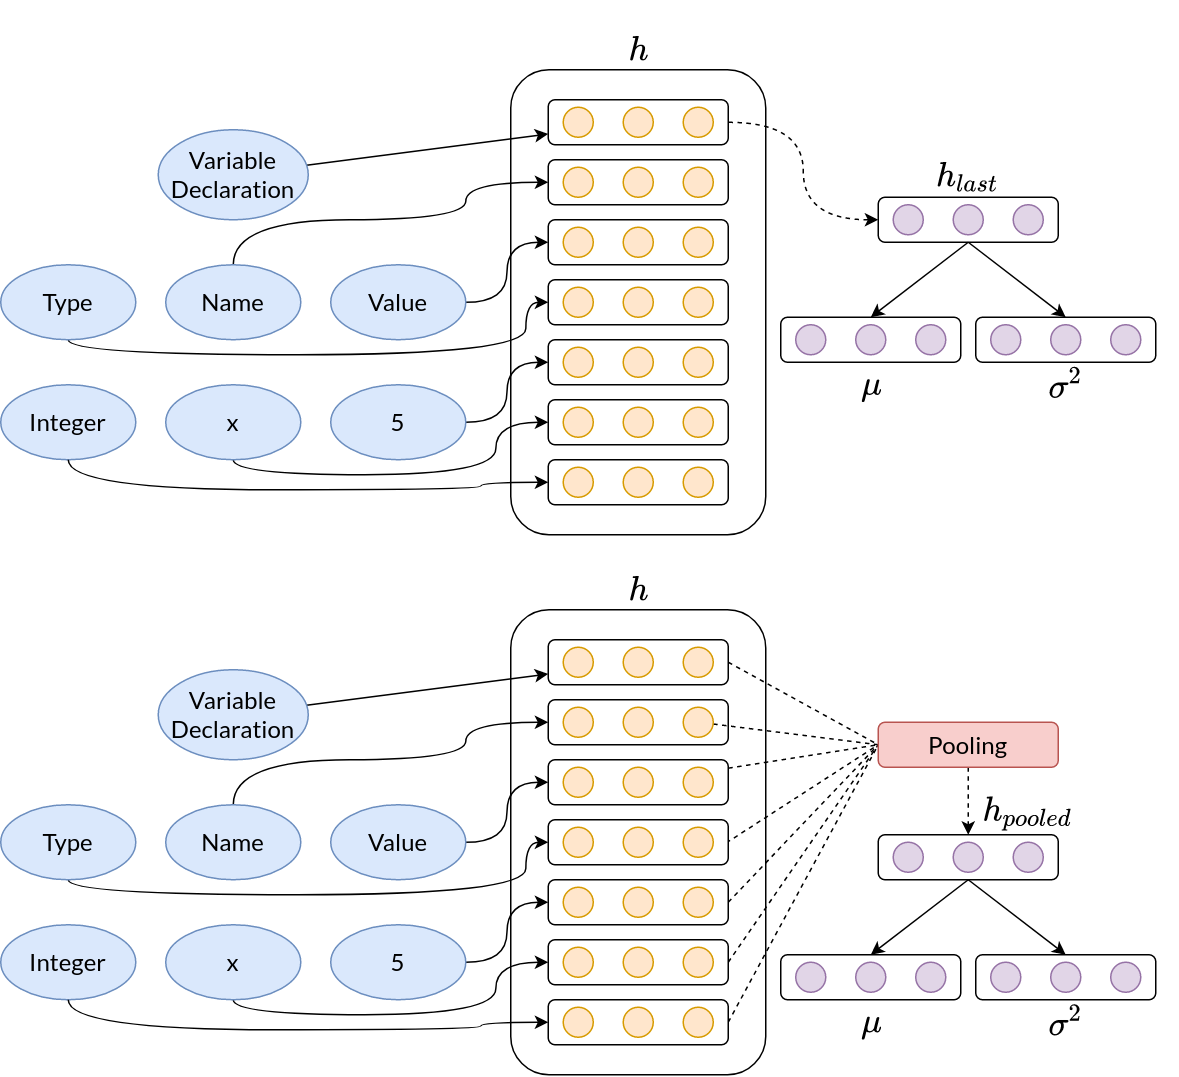
\includegraphics[width=\linewidth]{pooling.png}
    \caption[RNN pooling]{\textbf{Top}: Typical architecture of encoder model of VAE in which only the last hidden state from the RNN is used to compute the mean $u$ and variance $\sigma^2$. \textbf{Bottom}: A pooling method to aggregate the hidden states from the RNN to compute the mean $u$ and variance $\sigma^2$.}
    \label{fig:pooling}
\end{figure}




\paragraph{Neural attention} Tree-LSTM layers are followed by an attention layer. 
The node importance calculation is based on \cite{winata2018attention}, and updates the hidden states as follows:
% Isn't this also \odot rather than \cdot?
\begin{align}
    \mathbf{h}_{at} = \mathbf{h} \cdot tanh(\mathbf{W} \cdot \mathbf{h} + \mathbf{b})
\end{align}

Here, $h$ denotes the hidden states of the last Tree-LSTM layer. This additional layer allows the network to prioritize nodes that contain the most information. 


\paragraph{Pooling} 
The last step in the architecture is the pooling layer responsible for compressing the sequence of $h_{at}$ into a fixed size vector. 
We rejected a common \cite{fabius2015variational} approach of only taking the last hidden state of the RNN as the input to the decoder due to the long-term memory loss problem \cite{kao2020comparison} and use max pooling instead, see figure \ref{fig:pooling}.



\paragraph{Sampling latent code} The pooled vector is then used to compute the mean and variance of the approximate posterior to sample a latent code $z$ with the help of the reparametrization trick \cite{kingma2013auto}. The mean and variance are computed using linear layers that learn a set of weights and biases. 




\subsection{Decoder}
The goal of the decoder network is to reconstruct a given input as accurately as possible, given the latent code produced by the encoder. 

\paragraph{Tree decoding} We use the same tree structure for decoding as we used for encoding. 
Having a reversed order of the input sequence compared to the reconstructed sequence has been shown in \cite{fabius2015variational} to improve the performance of the model. 
We employ this technique in our model, which means that since our encoder processes trees bottom-up, the decoder will produce trees top-down. 
The idea here is that the first steps of decoding the tree are more related to the latent space than the last steps.



A method called the doubly-recurrent neural network (DRNN) \cite{alvarezmelis2017tree} allows for top-down tree generation from an encoded vector representation. This method operates solely on the vector representation and does not require that either the tree structure or the nodes are given. The DRNN is based on two recurrent neural networks, breadth and depth-wise, to model ancestral and fraternal information flow. For some node $y$ with parent $pa(y)$ and previous sibling $s(y)$, the ancestral and fraternal hidden states are computed as follows:

\begin{align}
    \mathbf{h}_a^y &= rnn_a(\mathbf{h}_a^{pa(y)}, \mathbf{i}^{pa(y)}) \\ \label{eq:ancestral_update}
    \mathbf{h}_f^y &= rnn_f(\mathbf{h}_f^{s(y)}, \mathbf{i}^{s(y)}) 
\end{align}

Where $rnn_a$, $rnn_f$ are functions that apply one step of the ancestral and fraternal RNNs, respectively. Furthermore, $\mathbf{i}^{pa(y)}$, $\mathbf{i}^{s(y)}$ are the input values (label vectors) of the parent and previous sibling respectively. After the ancestral and fraternal states of $y$ have been computed with the observed labels of its parent and previous sibling, these states can be combined to form a predictive hidden state:

\begin{align}
    \mathbf{h}^y_{pred} = \tanh\left((\mathbf{W}_a \cdot \mathbf{h}_a^y + \mathbf{b}_a) + (\mathbf{W}_f \cdot \mathbf{h}_f^y + \mathbf{b}_f)\right)
\end{align}

Where the operations applied to $\mathbf{h}_a^y$, $\mathbf{h}_f^y$ are linear layers with learnable weights and biases. This combined state then contains information about the nodes' surroundings in the tree.



For each node in the tree, the model needs to decide whether it has offspring and whether it has any successor siblings. We can use the predictive hidden state of a node $\mathbf{h}^y_{pred}$, with a linear layer and a sigmoid activation to compute the probability for offspring and successor siblings as:

\begin{align}
    p_a^y &= \sigma(\mathbf{W}_{pa} \cdot \mathbf{h}_{pred}^y + \mathbf{b}_{pa}) \label{eq:prob_ancestral} \\
    p_f^y &= \sigma(\mathbf{W}_{pf} \cdot \mathbf{h}_{pred}^y + \mathbf{b}_{pf})\label{eq:prob_fraternal}
\end{align}

During training, we use the actual values for whether a node has children and successor siblings. 
During inference, we can either greedily choose any confidence level to continue creating offspring and succeeding siblings by checking whether the probability is above some threshold or sample this choice. 



Besides topological predictions, the model should also predict the label of each token. Again the predictive hidden state can be used for label prediction as follows:

\begin{align}
    \mathbf{o}^y =  softmax\left(\mathbf{W}_o \cdot \mathbf{h}_{pred}^y + \mathbf{b}_{o}\right) \label{eq:label_pred}
\end{align}


\paragraph{Tree decoding optimizations} Now that we have the basic DRNN model \cite{alvarezmelis2017tree} in place to generate a tree from scratch using a latent vector, we can optimize it for our use case. 



The first issue is the possibly infinitely large vocabulary that source code allows. Since progam behavior is invariant to identifier replacement we map each unique identifier to a reusable ID \cite{tufano2019learning} and treat the prediction of identifiers as a clustering problem between declarations and references. We use the predictive hidden states of the nodes to learn relationships between declarations and references.  



The model can keep track of a list of the declared identifiers while generating an AST. Each time a new identifier is declared, a new reusable ID is added to the list. Then for each reference, we can compute the similarity to each of the declared identifiers using some similarity function and predict the most similar identifier. We can keep track of what type of node we are currently trying to predict due to the AST structure and because we have access to the parent node label, i.e., the parent node indicates whether the child node is a declaration or reference. Let $D$ be the set of currently declared identifier nodes and $y$ be the current reference node we are trying to predict, the most similar declared identifier can be computed as follows:

\begin{align}
    \mathbf{s}^{yz} &= similarity(\mathbf{W}_c \cdot \mathbf{h}^y_{pred} + \mathbf{b}_c,  \mathbf{W}_c \cdot \mathbf{h}^z_{pred} + \mathbf{b}_c) \\
    \mathbf{r}^y &= \min_{z \in D}(\mathbf{s}^{yz})
\end{align}



We have a similar problem for literal tokens; developers can use an almost infinitely large number of unique literals in source code. However, in contrast to identifier tokens, literal tokens influence the functionality of a program. Therefore, to assure that generated programs are still compile-able, we cannot remap the literal tokens to reduce the token count. For example, we cannot map rarely used literals to special unknown tokens, as unknown tokens create compiler errors. Instead, we can employ adaptive softmax \cite{grave2017efficient} to use a vocabulary consisting of many unique literal tokens without a considerable increase in computational complexity.



We have identifiers and literals as token categories already, but we can also categorize the leftover tokens into the following categories:

\begin{itemize}
    \item \textbf{Reserved tokens:} for, if, while, ...
    \item \textbf{Types:} int, long, string, ...
    \item \textbf{Built in function names:} printf, scanf, push, ...
\end{itemize}



In total, the five categories cover all the different tokens of the programming language (at least for C++). The reason for splitting up the leftover tokens into more categories is to predict these categories separately based on their parent node. For example, this ensures that we do not input a type-token in the tree, where there should be a reserved token. The categorization improves the compilation rate of the generated programs by allowing the model only to predict tokens of the correct token category. The tree-structured representation during decoding allows us to use this optimization technique. For the reserved tokens, type, and built-in function names, equation \ref{eq:label_pred} is used for label prediction, as there is only a limited number of unique tokens in these categories. 



To allow for the categorized label predictions, we need to add one more element to the DRNN model. 
An essential aspect of the tree structure is that identifiers, built-in function names, and literals occur in the leaves of the trees. 
Hence if a node has offspring, the category of the current node must be a reserved token. 
However, if a node has no offspring, it can be either of the categories, and we need to somehow decide which category to predict a label for. Note that a reserved token can also be on a leaf node on the tree. For example, consider an empty return statement. For that reason, similar to the topology predictions, we have the model predict whether a node is of the reserved token category or not. This prediction  is computed in the same way as the topology predictions using the predictive hidden state of the node as follows: 

\begin{align}
    p_r^y &= \sigma(\mathbf{W}_{pr} \cdot \mathbf{h}_{pred}^y + \mathbf{b}_{pr}) \label{eq:res_pred}
\end{align}



\paragraph{Add gate} The DRNN model has a large flaw, where it is not able to differentiate between paths with the same prefix. For example, consider the situation depicted in figure \ref{fig:treeAddGate}, where we have two function declarations named `add' and `main'. Due to the information flow downwards, both name nodes have the same hidden state and the model is not able to distinguish the leaf nodes and will therefore predict the same label for both. This issue is depicted in the left image of figure \ref{fig:treeAddGate}. To solve this issue, we would like to incorporate the fraternal states in the downwards flow for the model to learn to differentiate the paths downwards. Hence we would like to revise eq. \ref{eq:ancestral_update}, where we take inspiration from the LSTM model and apply the idea of the add gate to our ancestral update formula as follows:

\begin{align}
    &\mathbf{m}_f^y = \sigma(\mathbf{W}_m \cdot \mathbf{h}_f^y + \mathbf{b}_m)\\
    &\mathbf{a}_f^y = tanh(\mathbf{W}_a \cdot \mathbf{h}_f^y + \mathbf{b}_a)\\
    &\mathbf{h}_a^y = \mathbf{h}_a^y + (\mathbf{a}_f * \mathbf{m}_f)
\end{align}

This update to the fraternal state is applied after predicting the label for node $y$, which is depicted in the right image of figure \ref{fig:treeAddGate}. Here, $a_f^y$ is the value of the transformation on the previous sibling state that should be added to the parent state, where the $tanh$ transforms it between -1 and +1 to mitigate exploding gradients. Furthermore, $m_f^y$ decides which elements should be added using a sigmoid function that outputs values between 0 and 1. By multiplying $a_f^y$ with $m_f^y$, the model can learn to decide what and how much to add from the previous sibling state to each parent state's element to help predict the next steps of the tree.


\begin{figure}[ht!]
    \centering
    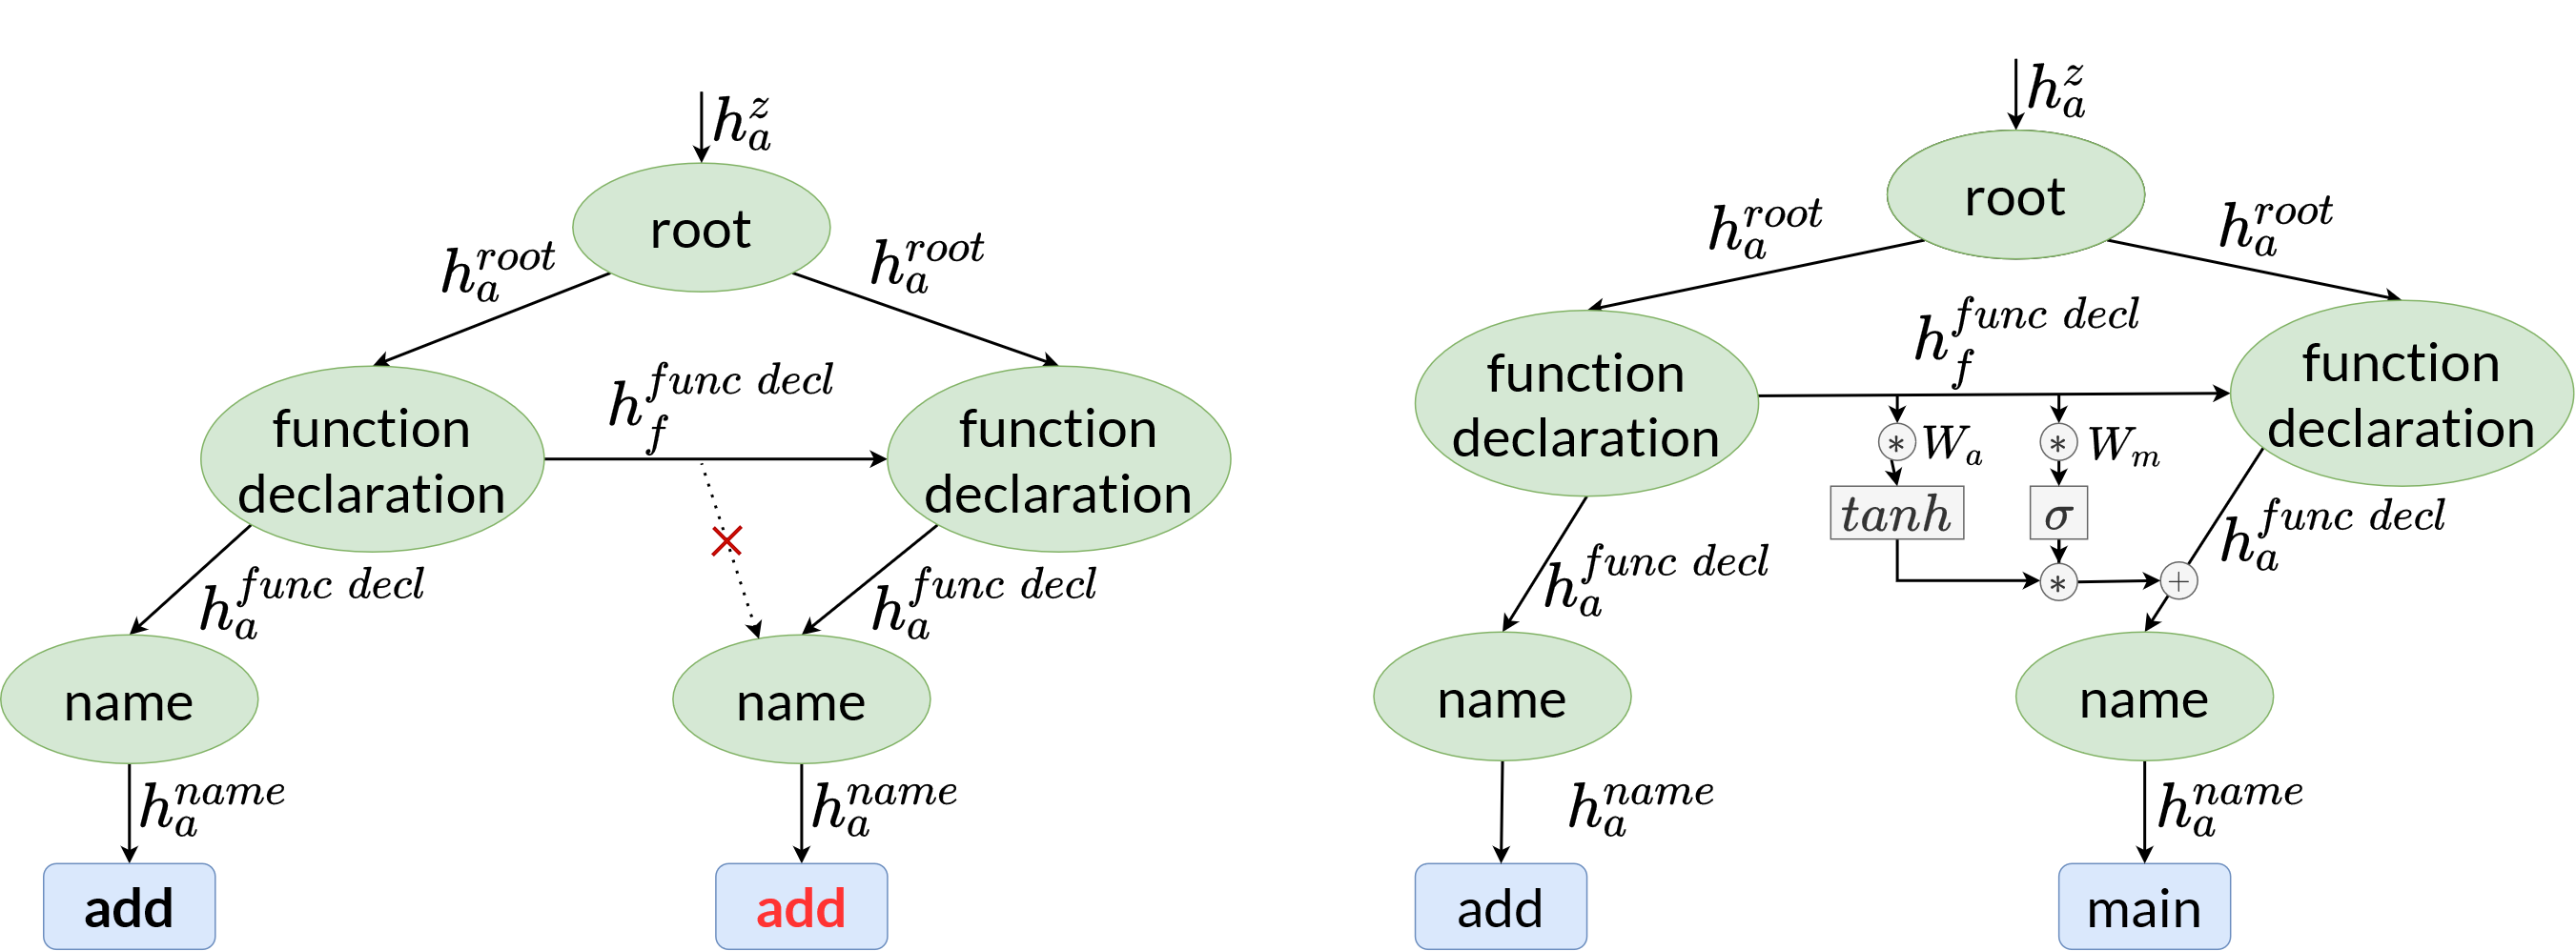
\includegraphics[width=\linewidth]{TreeAddGate.png}
    \caption{DRNN expanded with an add gate to allow for information flow from previous siblings downwards}
    \label{fig:treeAddGate}
\end{figure}

% TODO: say that the model allows for batching
% This is actually an advantage we have
%\subsection{Batching}
%We employ batching in the encoder and decoder to allow for efficient computation on GPUs. In the encoder, the computation of a node in the tree is dependent on all of its children. Therefore, the tree is processed bottom-up, and the trees can be processed in layers. For the decoder process, each node has two dependencies: the parent node and the previous sibling. Here, we process the tree top-down and from left to right at the same time. Note that each first child\footnote{With the first child, we refer to the left-most child} does not have a previous sibling. Therefore, each time a node is processed, its first child node can be computed in the next step. Moreover, because sibling nodes have the same parent, the direct successor sibling may also be computed in the next step. Hence, after processing a node, assuming the node has any offspring and successor siblings, the first child and successor sibling can be computed in the next time step.

% 

% For identifier tokens, the decoder model deviates slightly from this batching process. Because we treat the prediction of the identifier tokens as a clustering problem, we need the predictive hidden states of all the already declared identifiers when predicting a reference. A reference to an identifier may be processed before the declaration of a variable in the current setup. However, for predicting the correct label of a reference, we need to process its declaration first. Therefore, we process the identifier nodes separately, only after all other nodes have been processed. The order in which the identifier nodes are processed is from left to right within a tree, node by node. We ensure that declarations are always processed before their references by processing the identifier nodes from left to right. We parallelize this operation again across multiple trees. An example of the process is depicted in figure \ref{:treeBatchingIdentifiers}.

\subsection{Optimization}

\subsubsection{Mitigating KL vanishing}
KL vanishing is a common issue when dealing with VAEs with a decoder parameterized by an auto-regressive model.
We mitigate it vanishing using cyclical KL cost annealing \cite{fu2019cyclical}. Furthermore, we apply pooling to the hidden states of the RNN network in the encoder. Long \textit{et al.} \cite{long2019preventing} show this pooling method can effectively prevent the posterior collapse issue. 

\subsubsection{Loss function}
Predicting whether a node has offspring and successor siblings are binary choices, so we can use binary cross-entropy to compute the loss for predicting the topology of the AST. 
Let $a^y$, $f^y$ represent the actual values of having offspring and successor siblings for node $y$, the topological losses for this node are then computed as follows:

\begin{align}
    \mathcal{L}_{a}(y) = - a^y \cdot \log(p^y_a) + (1 - a^y) \cdot \log(1 - p^y_a) \\
    \mathcal{L}_{f}(y) = - f^y \cdot \log(p^y_f) + (1 - f^y) \cdot \log(1 - p^y_f)
\end{align}

\noindent where $\mathcal{L}_{a}$, $\mathcal{L}_{f}$ denote the ancestral and fraternal loss respectively. Because the reserved token category prediction (eq. \ref{eq:res_pred}) is so similar to the topological predictions, the loss for that component can be defined in a similar fashion:

\begin{align}
    \mathcal{L}_{r}(y) = - r^y \cdot \log(p^y_r) + (1 - r^y) \cdot \log(1 - p^y_r)
\end{align}

\noindent where we define $r^y$ to represent the actual value of node $y$ being in the reserved token category. 



Label prediction is a classification problem for all label categories, except the identifiers.
Hence, we can compute the cross entropy loss (or negative log likelihood):

\begin{align}
    \mathcal{L}_{l}(y) = - \log(\mathbf{o}^y[l^y])
\end{align}

\noindent where we assume that $l^y$ is the index of the true label, and hence $\mathbf{o}^y[l^y]$ retrieves the softmax value at the index of the correct class. 

Lastly, since predicting the labels of identifier (reference) tokens is treated as a clustering problem, we can use triplet loss \cite{chechik2010large}. 
To compute the loss of a reference node $y$, we select the true declaration node $z$ and sample a negative declaration node $x$; the loss is then defined as follows:

\begin{align}
    \mathcal{L}_i(y)=\max(\mathbf{s}^{yx} - \mathbf{s}^{yz},0)
\end{align}

\noindent We can then combine all of the separate components to form a single reconstruction loss function for a node:

\begin{small}
\begin{align}
   \mathcal{L}_{rec}(y) = 
\begin{cases}
    \mathcal{L}_{a}(y) + \mathcal{L}_{f}(y) + \mathcal{L}_{r}(y),& \text{if } y \text{ is a declaration} \\
    \mathcal{L}_{a}(y) + \mathcal{L}_{f}(y) + \mathcal{L}_{r}(y) + \mathcal{L}_{i}(y),& \text{if } y \text{ is a reference} \\
    \mathcal{L}_{a}(y) + \mathcal{L}_{f}(y) + \mathcal{L}_{r}(y) + \mathcal{L}_{l}(y),& \text{otherwise}
\end{cases}
\end{align}
\end{small}

Because the loss is decoupled, this allows us to weigh the objectives differently to emphasize, for example, topology or label prediction accuracy. We leave experimenting with different weights for objectives as future work. 

The total loss function, combining the KL divergence, KL weight $w$ and reconstruction loss becomes:

\begin{align}
    \mathcal{L}(N) = \mathcal{L}_{tot\_rec}(N) = \sum_{y \in N}\mathcal{L}_{rec}(y) - w \cdot D_{KL}\left(Q(z|N)||P(N)\right)
\end{align}

During training, we perform teacher forcing, technique that is commonly used with sequence generation.

\begin{figure*}[ht!]
    \centering
    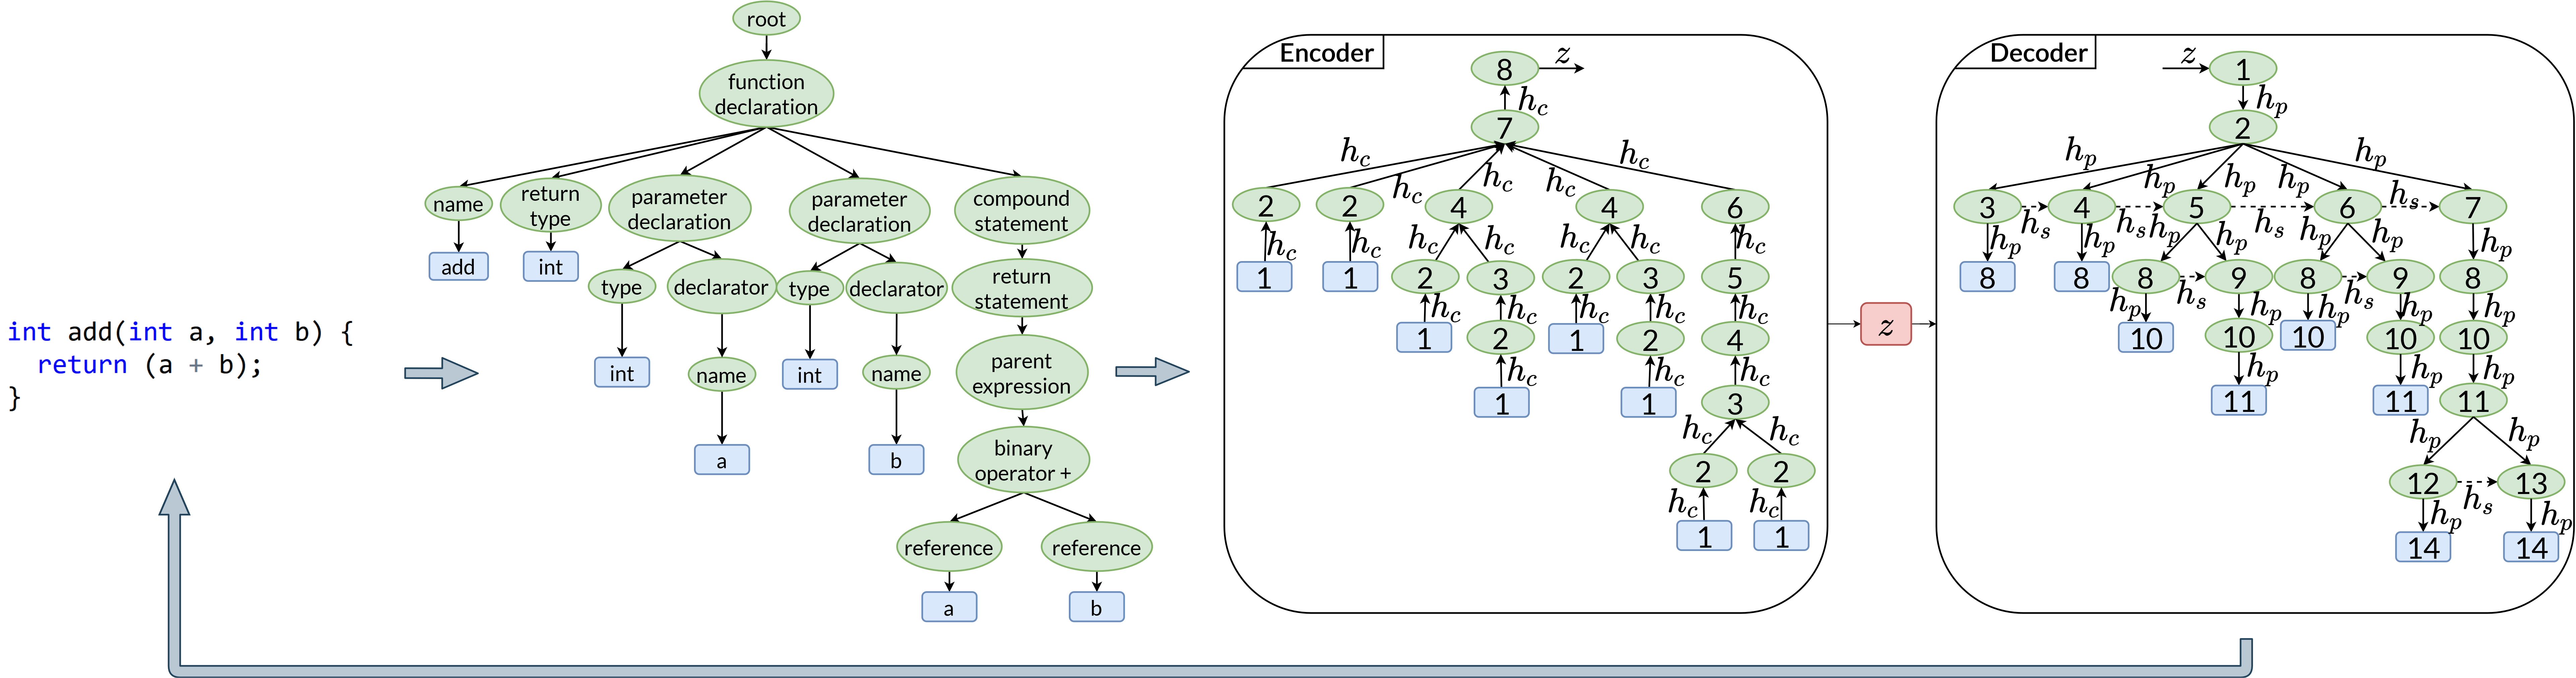
\includegraphics[width=\linewidth]{tree2treeLSTM2.png}
    \caption[Tree2Tree model high-level overview]{Tree to tree autoencoder overview. \textbf{First Fig.}: The piece of code considered. \textbf{Second Fig.}: The piece of code parsed to an AST tree format. \textbf{Third Fig.}: The order in which the encoder module encodes the tree structure bottom-up. Here, $h_c$ indicates the hidden state that travels from a child to a parent. \textbf{Fourth Fig.}: The order in which the decoder module decodes the tree structure top-down. Here, $h_p$ indicates the hidden state that travels from a parent to a child, and $h_s$ indicates the hidden state that travels from a node to its successor sibling.}
    \label{fig:tree2treeVAE}
\end{figure*}

\section{Evaluation}
\label{evaluation}

\subsection{Dataset}
We train and evaluate our model on a dataset of programs from code competition websites. Programs from these platforms exhibit a few qualities that are suitable for program synthesis. The programs are tested and known to be syntactically correct and compile-able, and they are standalone code fragments and do not depend on any code that is not built into the programming language. The dataset consists of almost two million C++ programs across 148 competitions divided over 904 problems. 

The programs in the data set are generally structured to contain a main function, standard input and output stream elements, computation and memory optimizations, and possibly some other elements such as helper functions/classes. Due to this general structure, the programs tend to overlap in their content, in contrast to, for example, natural language sentences. 

\subsection{Baseline}
Our method is compared to a baseline inspired by autoencoders used for text generation in natural language. We can also evaluate how well these models generalize to source code synthesis by taking inspiration from natural language models. The model architecture is inspired from \cite{bowman2015generating}. In this architecture, both the encoder and decoder networks contain single-layer recurrent neural networks. A Gaussian prior is used for the regularization of the latent space. The model operates on the original sequences of source code and decodes the latent vector back to the source code without an intermediate structured representation. Therefore we refer to the baseline model as the Sequence-to-Sequence (Seq2Seq) model, and the architecture is depicted in figure \ref{:seq2seq}.

\begin{figure*}[ht!]
    \centering
    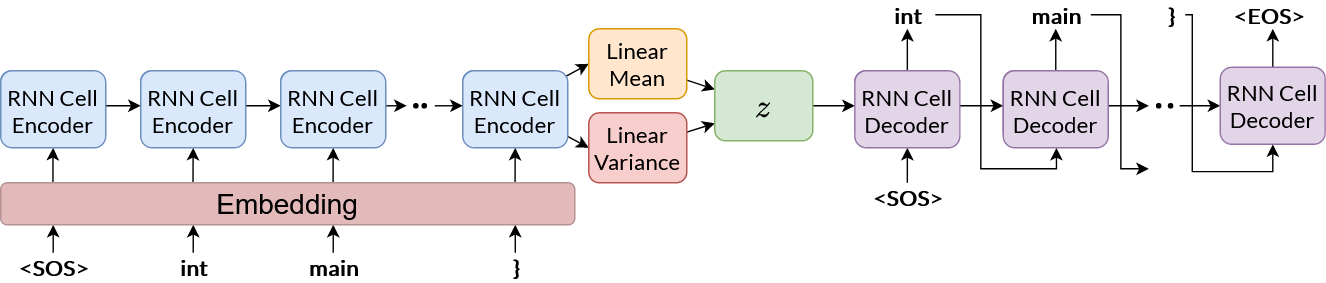
\includegraphics[width=0.8\linewidth]{seq2seq.png}
    \caption{The architecture of the Seq2Seq model}
    \label{fig:seq2seq}
\end{figure*}

Similar to our proposed autoencoder model, we employ methods to mitigate KL-vanishing. Again, we use cyclic KL annealing \cite{fu2019cyclical}, and we combine this with a technique called word dropout \cite{bowman2015generating} to weaken the decoder.

We use three-layered LSTMs in the encoder and decoder with a recurrent dropout rate of 20\% to reduce over-fitting. The embedding layer is initialized with Glove wiki gigaword 50 \cite{pennington2014glove} embedding. We train the model using the Adam optimizer \cite{kingma2014adam} with a learning rate of $1e-3$ and 10 epochs with early stopping and a patience of 3. We train and run the experiments on GPUs with a batch size set to 32.

\subsection{Reconstruction results}\label{sec:recon-results}
First of all, we look at how accurately the autoencoders can reconstruct programs. We use a separate test split containing around 60.000 samples of our data set to evaluate this and use these samples as input for the autoencoders. 



We compute BLEU scores \cite{papineni2002bleu} for both models on the original representation of the source code to obtain comparable results, i.e., we do not use the tree representation. The Tree2Tree model thus has an extra step to use the data parser to transform the tree representation back to source code. This extra step is disadvantageous for the Tree2Tree model as it may introduce some errors due to imperfections in the parsing process. The BLEU scores are then computed on each token in a program: keywords, identifiers, operators, and special symbols such as semicolons or braces. We report on the cumulative BLEU-1 through BLEU-4 scores to indicate the overlap between original and reconstructed programs. Furthermore, we present the percentage of reconstructed programs that compile to indicate how well the models have learned the programming language's syntax. We experiment with different combinations of latent sizes $l$ and hidden RNN dimensions $h$:  ($l$:10,  $h$:50), ($l$:50, $h$:100), ($l$:100, $h$:200), ($l$:150, $h$:300), ($l$:300, $h$:500), ($l$:500, $h$:800), ($l$:800, $h$:1200).



We use greedy decoding in reconstruction experiments (table table \ref{:rec_results}) to maximize accuracy. In contrast, sampling is used in generation tasks where diversity of candidates can be helpful.

\begin{table}[ht!]
\centering
% A table with adjusted row and column spacings
% \setlength sets the horizontal (column) spacing
% \arraystretch sets the vertical (row) spacing
\begingroup
\setlength{\tabcolsep}{3pt} % Default value: 6pt
\renewcommand{\arraystretch}{1.4} % Default value: 1
\begin{tabular}{cccccccc}
 & \textbf{Latent} & \textbf{BLEU-1} & \textbf{BLEU-2} & \textbf{BLEU-3} & \textbf{BLEU-4} & \textbf{Compiles}\\ \hline
\multirow{7}{*}{Seq}    &   10   &  0.037   &    0.024     &     0.017     &    0.013       &    0.000\%   \\
                            &   50   &      0.085    &      0.061         &         0.047      &    0.037       &       42.467\%      \\
                            &   100   &  0.295   &      0.225     &     0.176      &    0.141       &   65.808\%               \\
                            &   150   &     0.278  & 0.211          & 0.165          & 0.131          &  66.971\%              \\
                            &   300   & 0.346                     &  0.262                        &     0.203                     &     0.161                     & 60.651\% \\   
                            &   500   &  0.421                   &      0.332                    &         0.263                 &      0.211                    &  90.329\% \\
                            &   800   &  0.429                   &      0.329                    &         0.253                 &      0.195                    &  \textbf{91.784\%} \\\hline
\multirow{7}{*}{Tree}  &   10   &  0.445  &    0.339     &     0.260     &     0.202      &   28.375\%    \\
                        &   50   &     0.417    &      0.317    &       0.242    & 0.189  &  23.256\% \\
                            &   100   &     0.423      &      0.323     &     0.251      &  0.200 &      30.429\%     \\
                            &   150   & \textbf{0.486} &     \textbf{0.382}    &  \textbf{0.302}     &      \textbf{0.243}    &   35.419\%           \\
                            &   300   &   0.457                 &     0.342                &      0.260                &     0.202                   & 35.054\% \\   
                            &   500   &     0.398                &      0.301             & 0.230      &             0.178             &            36.022\%      \\
                             &   800   &     0.258                &      0.182             & 0.131      &             0.096             &     2.358\%      \\
\end{tabular}
\endgroup
\caption{Reconstruction results.}
\label{tab:rec_results}
\end{table}

The results listed in table \ref{:rec_results} show the superiority of the Tree2Tree model in terms of reconstruction capability (BLEU scores), especially for smaller latent sizes. The reconstruction scores of the Tree2Tree model of latent size 150 outperform all the Seq2Seq models up to latent size 800. In contrast, the Seq2Seq models show to perform much better at constructing compile-able programs, which improves with the model's size, to nearly 100\%. This is a surprising result, which is investigated in more detail in section \ref{evaluation}.

 


An interesting result is that the performance of the models does not necessarily increase with the size of the model. Especially for the Tree2Tree models, we see that after latent size 150, the models' performance decreases. In general, one would expect that the model would perform better with an increase in latent size, allowing more information flow between the encoder and decoder. We hypothesize that, because not only the latent size increases but also the number of hidden units in the auto-regressive models, the models experience KL vanishing. Due to the increasing hidden units, the auto-regressive models become stronger and may depend more on their predictions, ignoring information from the latent vector. In turn, the reconstruction performance vastly decreases. Confirmation of this hypothesis is left as a venue for future work.



Next, we would like to experiment on how different input sizes affect the performance of both models. Due to the tree-structured representation used by the Tree2Tree model, the size of the sequences that the RNNs process scale proportionally to the width and depth of the tree. The Seq2Seq model, on the other hand, processes sequences left to right, hence the number of computations of the RNNs scale directly with the sequence length. 



To evaluate the performance on different sized inputs, we split the test data set into three subsets. A small, medium and large subset with the following properties:

\begin{itemize}
    \item \textbf{small subset}: maximum of 250 tokens
    \item \textbf{medium subset}: between 251 and 500 tokens
    \item \textbf{large subset}: between 501 and 750 tokens
\end{itemize}

 

We compute the BLEU scores and compilation percentage again using greedy decoding on the smaller subsets for the best performing Seq2Seq and Tree2Tree models, based on the results of table \ref{:rec_results}. Here, performance is based on the combination of BLEU-4 and compilation percentage. For Seq2Seq, this is the model with latent size 500. Similarly, for Tree2Tree, this is the model with latent size 150. The results are depicted in table \ref{:rec_results_inp_sizes}.



%150 latent t2t lr 0.001 large test set (> 500, <= 750): bleu1 0.317, bleu2 0.236, bleu3 0.177, bleu4 0.134, compiles 5.001

%150 latent t2t lr 0.001 medium test set (> 250, <= 500): bleu1 0.468, bleu2 0.364, bleu3 0.284, bleu4 0.225, compiles 21.241


\begin{table}[ht!]
\centering
% A table with adjusted row and column spacings
% \setlength sets the horizontal (column) spacing
% \arraystretch sets the vertical (row) spacing
\begingroup
\setlength{\tabcolsep}{3pt} % Default value: 6pt
\renewcommand{\arraystretch}{1.4} % Default value: 1
\begin{tabular}{clccccc}
 & \textbf{Input} & \textbf{BLEU-1} & \textbf{BLEU-2} & \textbf{BLEU-3} & \textbf{BLEU-4} & \textbf{Compiles}\\ \hline
\multirow{3}{*}{Seq}    &   small   &   0.513  &    0.403    &      0.321    &  0.258      &  95.334\%     \\
                            &   medium   &  0.306      &    0.244        &      0.192     & 0.153      & 86.812\% \\
                            &   large   &    0.196   &      0.157   &   0.123       &   0.096       &  87.971\% \\ \hline
\multirow{3}{*}{Tree}  &   small   &   0.633  &    0.516     &     0.424     &     0.355      &  59.022\%                \\
                            &   medium   &   0.478  &   0.371        &          0.289 &     0.229   & 21.241\%            \\
                            &   large   &  0.324 &      0.242  & 0.181    &    0.138     &    5.001\%         \\ 
\end{tabular}
\endgroup
\caption{Reconstruction results of the best models on different input sizes.}
\label{tab:rec_results_inp_sizes}
\end{table}



From table \ref{:rec_results_inp_sizes} we can observe that both models follow the same logical trend: the larger the input size, the lower BLEU-scores and compilation percentages. For the Tree2Tree model, the BLEU scores for the medium subset seem to be similar to the BLEU scores on the entire test set, whereas, for the Seq2Seq model, the BLEU scores are much lower on the medium subset. The models seem to be fairly close in terms of performance degradation from small to large program sizes. For example, we can measure performance degradation for the large versus small subset by dividing the BLEU-4 scores on the large set by the BLEU-4 score on the small set. For the Seq2Seq model, we get a score of $0.372$, and for the Tree2Tree model, we get $0.389$. Similarly, we get $0.593$ and $0.645$ for the Seq2Seq and Tree2Tree model for the medium versus small subset. While the performance degrades less with increasing input sizes for the Tree2Tree model, this difference is insignificant. 



An issue with the aforementioned computation of performance degradation is that it does not correct for elements in programs that are almost always present. For example, each program contains a main function, with standard input and output streams. The models may simply always predict these standard elements of a program and then use the information of the encoder to complete the details of the program. However, this causes the BLEU score to consist of two parts: the score for the prediction of the elements that are always present and the score of what it has learned to predict together with the encoder. The latter is more interesting and shows how much information can be saved in the latent vector. 



Therefore, we apply a correction on the BLEU scores to focus on the prediction based on the information in the latent vector. We compute corrected scores by feeding the decoder with random latent vectors and computing BLEU scores on the subsets of the test data set. Then, we subtract these correction scores from the computed BLEU scores in table \ref{:rec_results_inp_sizes}, and take 0 if the result of the subtraction is negative. The corrected BLEU scores including the correction scores are presented in table \ref{:corrected_rec_results_inp_sizes}.

\begin{table}[ht!]
\centering
% A table with adjusted row and column spacings
% \setlength sets the horizontal (column) spacing
% \arraystretch sets the vertical (row) spacing
\begingroup
\setlength{\tabcolsep}{3pt} % Default value: 6pt
\renewcommand{\arraystretch}{1.4} % Default value: 1
\resizebox{\linewidth}{!}{%

\begin{tabular}{clccccc}
\textbf{Model}   & \textbf{Input size} & \textbf{BLEU-1} & \textbf{BLEU-2} & \textbf{BLEU-3} & \textbf{BLEU-4} \\ \hline
\multirow{3}{*}{Seq2Seq}    &   small   &   0.072 (0.441)  &    0.077 (0.326)    &  0.075    (0.246)    &  0.070 (0.188)     \\
                            &   medium   & 0.006 (0.300)      &  0.018  (0.226)        &    0.021  (0.171)     & 0.023 (0.130)    \\
                            &   large   &   0.000 (0.213)   &  0.000    (0.166)   & 0.000  (0.128)       &  0.000 (0.099)   \\ \hline
\multirow{3}{*}{Tree2Tree}  &   small   &  0.200 (0.433)  &  0.220  (0.296)     &  0.223   (0.201)     &    0.218 (0.137)        \\
                            &   medium   &  0.148 (0.330)  &  0.147 (0.224)        & 0.146 (0.150) &    0.128 (0.101)        \\
                            &   large   &  0.102 (0.222) &    0.090  (0.152)  &  0.079 (0.102)     &  0.070  (0.068)      &   \\
\end{tabular}%
}
\endgroup
\caption{Corrected BLEU scores of reconstructed results of the best models on different input sizes. (correction scores in parenthesis)}
\label{tab:corrected_rec_results_inp_sizes}
\end{table}



table \ref{:corrected_rec_results_inp_sizes} indicates a large difference in performance degradation between the Seq2Seq model and the Tree2Tree model. A noticeable result is that the corrected BLEU scores for large programs predicted by the Seq2Seq model are 0. Hence, the Seq2Seq model extracts no information from the latent vector at all for large programs. Similarly, for medium-sized programs, little information is transferred between the encoder and decoder. We can again compute the performance degradation scores for the Seq2Seq model, which are $0.280$ and $0.00$ for the medium versus small and large versus small subsets, respectively, on the corrected BLEU-4.



In contrast, the performance degradation is much smaller for the Tree2Tree model:  $0.587$ and $0.321$ for the medium versus small and large versus small subsets, respectively, on the corrected BLEU-4. Hence, the structural nature of the Tree2Tree model scales better to large input sequences than the Seq2Seq model in terms of reconstruction scores, even with a much smaller latent size. 



An interesting observation is that the latent vector conveys relatively little information in terms of BLEU scores. The correction scores make up a large part of the total BLEU scores as presented in table \ref{:rec_results_inp_sizes}. Hence, the BLEU scores are largely determined by the models' general knowledge of how C++ programs are built up and not the specific content.

\subsection{Generative results}
\label{results:gen}
To see how well autoencoders can generate reasonable samples from any point in latent space that conform to the C++ syntax, we sample 1000 random latent vectors from the prior distribution $\mathcal{N}(0, I)$ and input these vectors to the decoder networks. Then, we compute the percentage of generated programs that compiles and is thus also syntactically correct.



We employ two decoding strategies to test the generative capabilities of the models: greedy decoding and sampling. The sampling strategy we apply is a combination of top-$k$, nucleus, and temperature sampling \cite{holtzman2019curious}. We first use temperature sampling to scale the logits to control the shape of the probability distribution. Then, we filter the on the top-$k$ samples, after which we filter tokens on their cumulative probability using nucleus sampling (top-$p$). Lastly, we sample a token from the resulting distribution. The selected sampling hyper-parameters for this experiment are: $k=40$, $p=0.9$, $temperature=0.7$. The results of the experiment are displayed in table \ref{:gen_results}.

\begin{table}[ht!]
\centering
% A table with adjusted row and column spacings
% \setlength sets the horizontal (column) spacing
% \arraystretch sets the vertical (row) spacing
\begingroup
\setlength{\tabcolsep}{3pt} % Default value: 6pt
\renewcommand{\arraystretch}{1.4} % Default value: 1
\begin{tabular}{cccc}
\textbf{Model}   & \textbf{Latent size} & \textbf{Greedy search} & \textbf{Sampling} \\ \hline
\multirow{5}{*}{Seq2Seq}    &   10   &  0.0\%   & 0.9\%  \\
                            &   50   &   38.5\%    &  2.9\%   \\
                            &   100   &   62.1\%   &  21.3\%     \\
                            &   150   &   58.0\%  &     23.5\%        \\
                            &   300   &  60.6\%  &  36.8\%   \\   
                            &   500   &  67.5\% & 37.8\% \\
                            &   800   & 78.2\%  & 39.6\% \\\hline
\multirow{5}{*}{Tree2Tree}  &   10   &   29.6\%   & 20.2\% \\
                            &   50    & 22.6\%   &  17.7\%    \\
                            &   100    & 30.3\%  &       22.1\%      \\
                            &   150  &  26.9\%  &   18.8\%     \\
                            &   300  & 23.4\%  & 12.8\%    \\   
                            &   500 & 25.6\%  & 14.4\%\\
                            &   800   &  4.1\% & 6.7\% \\
\end{tabular}
\endgroup
\caption{Generative results compilation percentage.}
\label{tab:gen_results}
\end{table}




The results from table \ref{:gen_results} show similar trends as section \ref{sec:recon-results}. The general trend is: the larger the model (in terms of latent size and hidden units), the higher the compilation percentage. Moreover, greedy search during inference gives a higher compilation percentage than sampling. This outcome is not surprising, as, with greedy search, we always pick the label for which the model is most confident. On the other hand, sampling gives a more varied output and may be useful for searching similar programs in a vicinity of the latent space. The trade-off for a more diverse output is thus a lower compilation ratio. 


\section{Conclusion}

Our results indicate that Tree Variational Autoencoders have a significant advantage over sequence-to-sequence models in low-dimensional latent spaces, achieving both a higher compilation rate and a higher reconstruction quality.
In higher-dimensional latent spaces seq2seq programs offer a higher compilation rate, but based corrected BLEU scores indicate that this benefit is often achieved by sacrificing reconstruction quality, even to the point of ignoring the input completely.

Overall, our findings support the initial hypothesis that structured autoencoder models are better suited for program synthesis than sequence-to-sequence alternatives.
We believe this result to be a significant step towards an autoencoder-based foundation model for genetic programming and genetic improvement of software.


\newpage
\chapter{A Multiagent Framework for Programming with Large Language Models}\label{ch:autocode-autoregr}
\section{Introduction}
\label{sec:intro}





Given these challenges, research in machine learning on source code~\cite{allamanis2018:survey} tends to focus on restricted domain-specific languages~\cite{chen2021:latent,polozov2015:flashmeta,liventsev2021:bf} or automating specific parts\footnote{~similarly to autonomous driving~\cite{grigorescu2020:survey,marcano2020:review}} of the software development process~\cite{lu2021:codexglue,niu2023:crosscodebench} such as code search~\cite{husain2020:codesearchnet}, code translation~\cite{roziere2020:unsupervised}, detection of issues~\cite{fernandes2016:reviewbased,chakraborty2021:deep}, improvement~\cite{petke2018:genetic} and repair~\cite{legoues2019:automated} rather than fully autonomous programming in a programming language popular with human developers~\cite{:tiobe}.
However, two recent innovations potentially make the latter task tractable.

\begin{figure*}
    \centering
    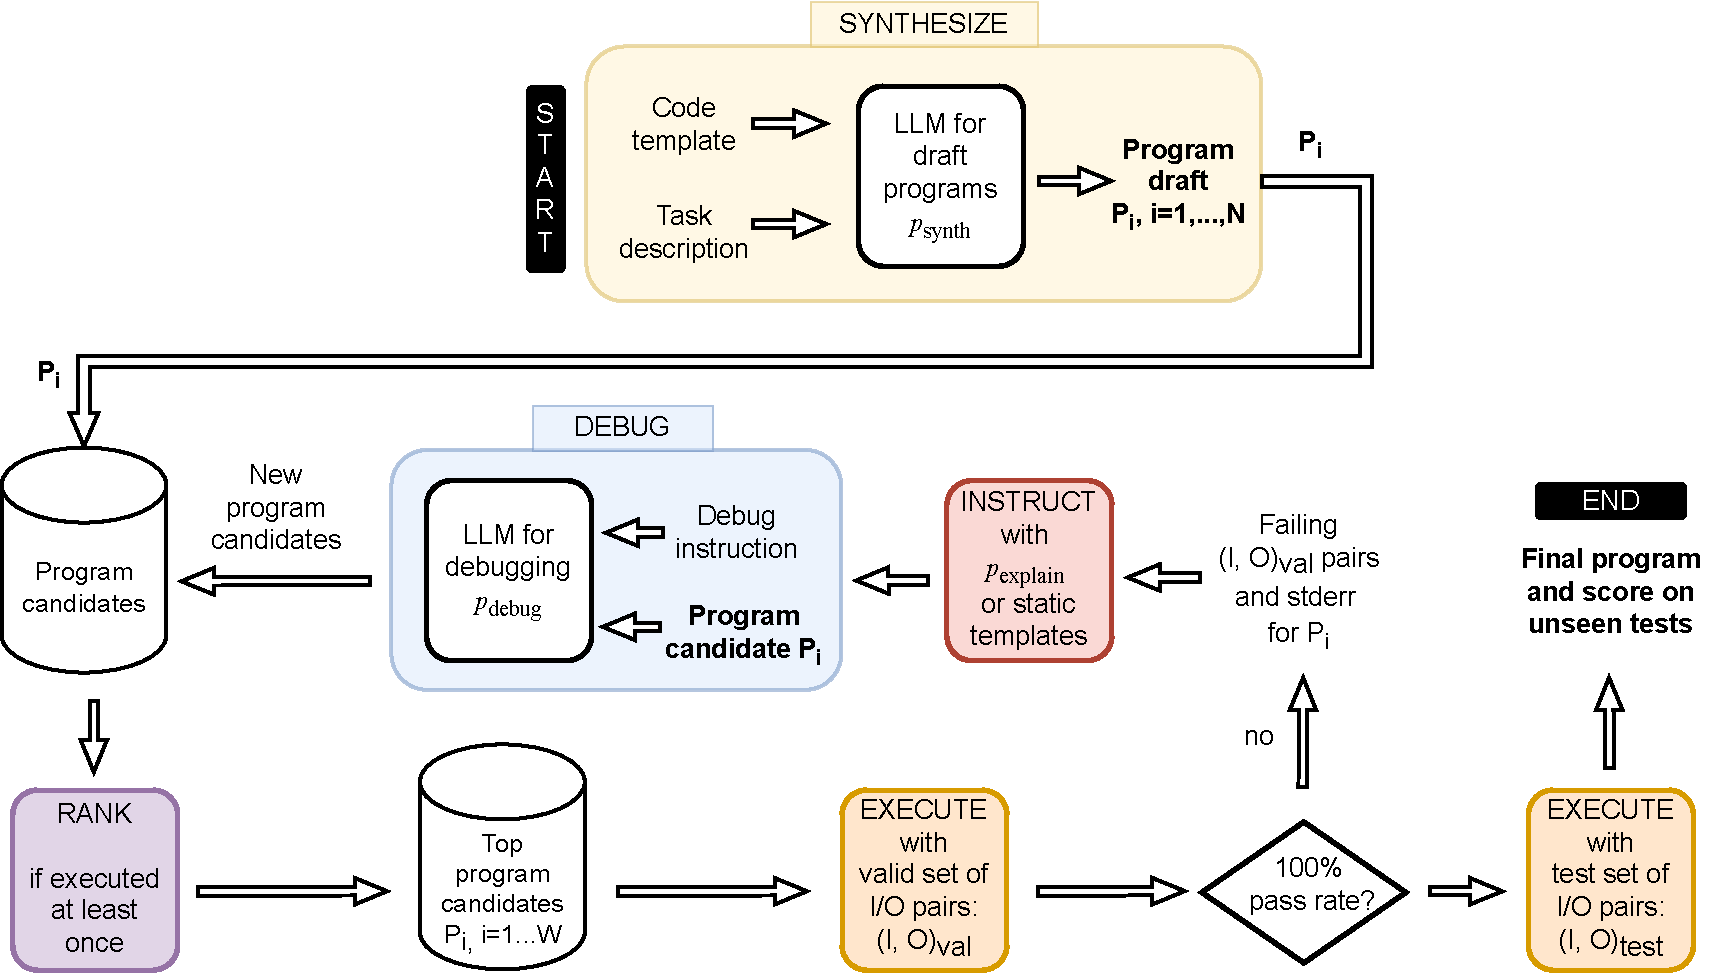
\includegraphics[width=\linewidth,trim={0mm 8mm 0mm 0mm}]{codex-for-psb-seidr-methodology-4.drawio.pdf}
    \caption{Overview of Synthesize, Execute, Instruct, Debug, and Rank}
    \label{fig:method}
\end{figure*}

One is \emph{Synthesize, Execute, Debug}~\cite{gupta2020:synthesize}, a framework that attempts to bridge the "last mile" gap by introducing program repair into the program synthesis algorithm. 
A programming task is specified using both a natural language description and a set of input/output (I/O) pairs demonstrating what output is expected of the program, thereby combining text to code ~\cite{iyer2018:mapping} and programming by example~\cite{halbert1984:programming,gulwani2016:programming} paradigms typical for competitive programming~\cite{zavershynskyi2018:naps}.
\emph{Synthesize, Execute, Debug} creates a first draft program using a generative model, compiles and executes it with given input examples.
This is followed by a program repair step to fix the identified errors.

Another relevant innovation is instruction fine-tuned large language models~\cite{ouyang2022:training}. Instruction fine-tuned models use human feedback in their training process and are designed to explicitly or implicitly admit two inputs: a source text (or code) and a textual command instructing the model to edit the source in a particular way, i.e., "summarize" or "translate to Python".
These models have been shown to be highly successful in automatic program repair~\cite{fan2023:automated}. 
However, given the free-form nature of these instructions\footnote{Throughout this paper we avoid other definitions of \emph{instruction}, such as \emph{an individual operation in code}, to prevent ambiguity.} how one should engineer instructions that maximize repair performance is an open question. 

Section~\ref{sec:methodology} presents a framework that adapts \emph{Synthesize, Execute, Debug} to instruction fine-tuned Large Language Models in agents for solving programming tasks in an autonomous fashion. 
We discuss related work in Section~\ref{sec:related-work}, introduce experiments to establish optimal search and prompting strategies for this framework in Section~\ref{sec:eval}. 
Finally, we demonstrate in Section~\ref{sec:results} that our framework outperforms conventional automatic programming techniques, such as genetic programming and naive application of large language models that generate one solution per problem without updating it iteratively. 

\section{Methodology}
\label{sec:methodology}
The proposed 5-agent framework, \emph{Synthesize, Execute, Instruct, Debug and Rank}, or \method{},\footnote{~seiðr also refers to a type of Norse magic~\cite{blain2002:nine} pertaining to predicting and controlling the future, which we deem thematically appropriate.} is summarized in figure \ref{fig:method}, which we discuss in detail in Section~\ref{sec:ingredients}.
To solve a programming task defined as a text description and a collection of I/O examples, we split I/O examples into prompt and validation sets and use the prompt set in a large language model to \synthesize{} a population of candidate solutions.
We \execute{} the solutions, test them against the validation set, generate a text description of the identified problems used to \instruct{} a large language model to produce repaired candidate solutions similar to the way a human developer \debug{}s a program.
We \rank{} the candidates
by correctness measured by matching I/O pairs, discard the worst candidates, and repeat until a fully correct solution is found.

 

\subsection{Ingredients}
\label{sec:ingredients}

\method{} makes use of instruction fine-tuned large language models: a \emph{synthesis} model \synthmodel{}, a \emph{debugging} model \debugmodel{}, as well as a model \textmodel{} that can be used for writing textual instructions, which are forwarded to the code generation model \debugmodel{} for code updates. 
Therefore, the setup can be described as two agents communicating with each other, whereby one generates code and another one provides critical or supervising comments on what should be changed in the generated code. 

The models \synthmodel{}, \debugmodel{}, and \textmodel{} can be either separate models or the same model.
The pre-requisites are that \synthmodel{} and \debugmodel{} models are able to understand natural language (descr) and partial or full programs (code) and generate code based on them. 
The model \textmodel{} should be able to understand code and natural language and either auto-complete or generate the debugging instruction from scratch. 
Note that the debugging instructions can be generated from failing tests using static templates 
%as described in~\cite{liventsev2023:fully}. 
However, we focus on the implementation in which an LLM generates debug instructions, which is also suitable for chat models in addition to instruction fine-tuned models. 
In general, \method{} requires a sequence-to-sequence generative model for these agents. 
We have chosen the state-of-the-art transformer models~\cite{vaswani2017:attention} for \synthmodel{}, \debugmodel{}, and \textmodel{} in our experiments as described in Section~\ref{sec:models}. 

Each LLM is a highly parameterised probability distribution over the space of (code, description)-tuples with parameters estimated on a large diverse (i.e., non-task-specific) corpus.
This stochastic nature of language models is an important prerequisite for \method{}, since it lets us sample batches of diverse candidate solutions from \synthmodel{}, \debugmodel{}, and \textmodel{}. 
We denote the number of generated outputs with $\treearitydraft{},$ $\treearitydebug{},$ and $\treearityexplain{},$ correspondingly.
Moreover, each model generates the most probable and less probable outputs in each batch, which helps diversify problem solving attempts. 
In the implementation-related sections further, we explain how we vary with the number of candidate solutions, debug instructions, and repairs generated in a batch by each LLM in \method{}.


\subsubsection{Synthesize}
\label{sec:synth}

\begin{figure}
    \centering
    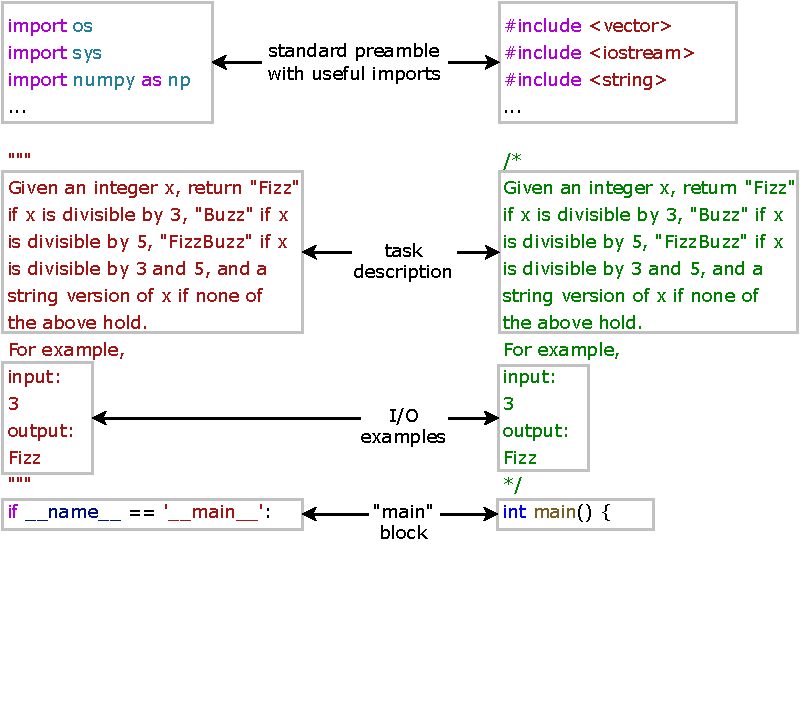
\includegraphics[width=0.7\linewidth, trim={0mm 40mm 0mm 0mm}, clip]{Templates-new-v2.pdf}
    \caption{Anatomy of \synthesize{} templates}
    \label{fig:template}
\end{figure}

The framework starts with the \synthesize{} agent, which is responsible for generating initial draft solutions to programming tasks to be repaired in the later stages of \method{}.
We start with a basic template for a chosen programming language that contains a number of standard library imports as shown in figure~\ref{fig:template}.
We populate this template with a comment indicating a text description of a task at hand and several I/O examples from the prompt training set.
We design the templates with prompt engineering guidelines\footnote{\url{https://platform.openai.com/docs/guides/prompt-engineering/six-strategies-for-getting-better-results}}$^{,}$ and prior work~\cite{debruin2021:autoencoders} in mind.
We then sample $\treearitydraft{}$ programs from \synthmodel{}, setting \texttt{code} to the populated template and \texttt{description} to the natural language description of what the model should generate.
We use temperature sampling with a monotonically increasing temperature schedule where $i$-th program is sampled with temperature $t_i \approx \frac{i}{\treearitydraft{}}$ (approximate equality enables efficient implementation by means of batching, i.e., generating several inputs with the same input pair of (code, descr)).
Thus, the sampling procedure for the first programs approximates deterministic maximum likelihood estimation.
Ultimately, this approach ensures that samples are diverse, but always contain the likeliest programs.

\subsubsection{Execute}
\label{sec:execute}

The \execute{} agent compiles the programs (if necessary) and launches them using the standard tools for the programming language.
The program is run once for every I/O pair in the validation set. 
Its \texttt{stdin} stream receives all the input lines in a given input pair, and its \texttt{stdout} and \texttt{stderr} streams are captured and saved.
We then measure the \emph{score} of the program defined as accuracy over output lines, with \expectedoutput{} being the expected output, and $n=\max\{|\expectedoutput{}|, |\text{stdout}|\}$:
\[    
\text{score}(\expectedoutput{}, \text{stdout}) = \frac{\sum^{n}_i{\mathbb{I}[\text{stdout}_i = O_i]}}{n} 
\]
unless \texttt{stderr} is non-empty during compilation or execution, which is considered to indicate failure and is assigned a score of 0.

\subsubsection{Instruct}
\label{sec:instruct}

The goal of the \instruct{} agent is to provide instructions that summarize bugs in a program candidate and suggest a solution for \debugmodel{}. 
Each call to \textmodel{} can result in $\treearityexplain{}\ge1$ instructions, a batch output of an LLM.
The resulting instruction(s) with the bug summary should indicate what requirement is violated and instruct the LLM to edit the candidate program so that the candidate meets the violated requirements. 

In \method{}, we generate instructions using template engines. 
In general, template engines replace placeholders in files or strings with input values and return a formatted string. 
With template engines, we can create templates that will be adapted dynamically based on the results of program candidate execution. 
The anatomy of the \instruct{} agent is shown in figure~\ref{fig:method-instruct}.
As inputs for templates, we use compiler or interpreter output if the exit code of the program is not zero, i.e., if the program finishes with an error.
Otherwise, if the exit code is zero but the candidate fails on a validation test pair $\left( I, O\right)_\text{val},$ the failing test case information is passed to the template. 
In the latter case, the program execution finishes well (exit code 0), which indicates absence of syntax or compiler/interpreter errors, but the logic of the program does not correspond to the expected behavior. 

In addition to providing a failing test case or \texttt{stderr}, one may choose to give the model \textmodel{} more context, such as the problem name, task description and the code generated so far. 
Prompt templates used for experiments are detailed in Section~\ref{sec:prompts}.

\begin{figure*}
    \centering
    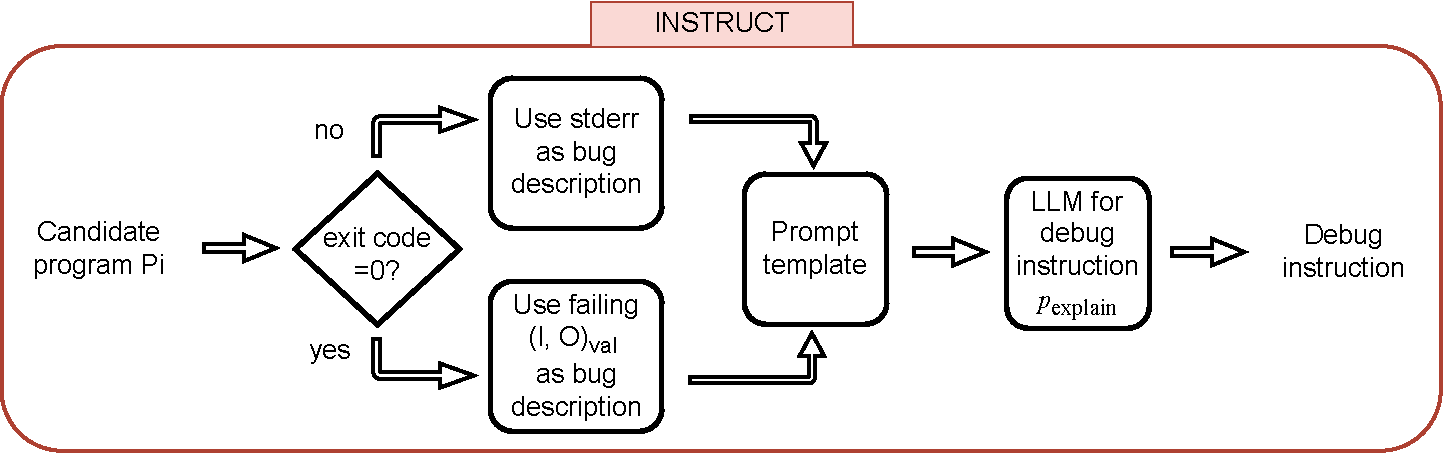
\includegraphics[width=.8\linewidth,trim={0mm 6mm 0mm 0mm}]{codex-for-psb-seidr-instruct-1.drawio.pdf}
    \caption{\instruct{} agent.}
    \label{fig:method-instruct}
    \vspace*{-3ex}
\end{figure*}

\begin{comment}
We consider two different designs of the instruction generation block: \instructs{} and \instructllm{} shown in figure~\ref{fig:method-instruct}. 
Both types of blocks use failing I/O pairs from the validation set and \texttt{stderr} output of the candidate execution. 
In both blocks, if \texttt{stderr} is not empty, i.e., execution errors occur before getting the output to compare it with the expected output, the \texttt{stderr}-based template engine generates an instruction to fix the error mentioned in \texttt{stderr}. 
However, the blocks differ in the way they transform failing I/O pairs to generate instructions in case \texttt{stderr} is empty.

\instructs{} uses a fixed input template and substitutes placeholders for input and output with the corresponding strings of the first failing test case.
We show the resulting instruction for an exemplar template in figure~\ref{fig:method-instruct}.
By contrast, \instructllm{} uses the failing I/O pair in the LLM for text completion, thereby prompting the text LLM to produce the bug summary. 
An exemplar output of the code behavior template engine in figure~\ref{fig:method-instruct} describes that the code returns output O instead of expected output O$_{\text{val}}$ for the failing test case with input string I$_{\text{val}}.$
The LLM is then prompted to auto-complete this description of program behavior with the bug summary. 
The bug description is passed further to the next template engine and used as the debugging instruction, such as ``\emph{Fix~\{bug summary\}}''.
\end{comment}

\subsubsection{Debug}

The main component of \method{} which addresses the "near miss syndrome" is the \debug{} agent.  
This agent iterates over all programs in the population to repair the candidate programs and pass more tests. 
It uses the instructions written by \instruct{} to sample from \debugmodel{} model $\treearitydebug{}$ times
to repair every candidate and create a new population of \treearity{} candidates.
For \debugmodel{}, the parameter \texttt{code} is set to the current version of the candidate solution and \texttt{descr} to the output of \instruct{} and any additional context chosen for a specific implementation.
The current generation of candidates is then replaced with \treearity{} outputs of \debug{}.

\subsubsection{Rank}

The \rank{} agent implements what is known in genetic programming as \emph{parent selection}~\cite{koza1994:genetic}: it selects the best $\beamwidth{}$ programs to be further improved by the \debug{} agent.
We consider 2 different parent selection algorithms: simple ranking and lexicase selection.

\emph{Simple ranking} sorts the programs by their average test score and selects top $\beamwidth{}$ candidates. 
Such ranking approach is a \emph{quality-based} selection method.
The programs are selected based on the intuition that repair of the best so far (but imperfect) programs begets good programs.

\emph{Lexicase selection}~\cite{helmuth2015:solving} is an approach from the \emph{quality diversity} family that maximizes diversity of selected candidates in addition to their score.
Lexicase selection ensures diversity by keeping the program candidates which perform the best on unique tests as opposed to the program candidates that perform best on average on all tests but, possibly, do not perform perfectly on any unique test.
The algorithm is as follows:
\begin{enumerate}
    \item randomly shuffle the set of tests;
    \item select a program with the best score on test 1;
    \item if several programs are tied, resolve the tie by selecting the best program on test 2;
    \item repeat for tests $3,4,\dots,$ until only one program is left;
    \item mark this program as "selected";
    \item if less than $\beamwidth$ programs are selected, go back to step 1.
\end{enumerate}
This ensures that even if the average quality of selected candidates is lower, the batch of $\beamwidth{}$ programs collectively contains a higher number of requisite "skills", as measured by tests.

See section~\ref{sec:lexicase-results} for their empirical comparison.

\subsection{Meaning of Hyperparameters}
\label{sec:beam-search}
\begin{figure}
    \centering
    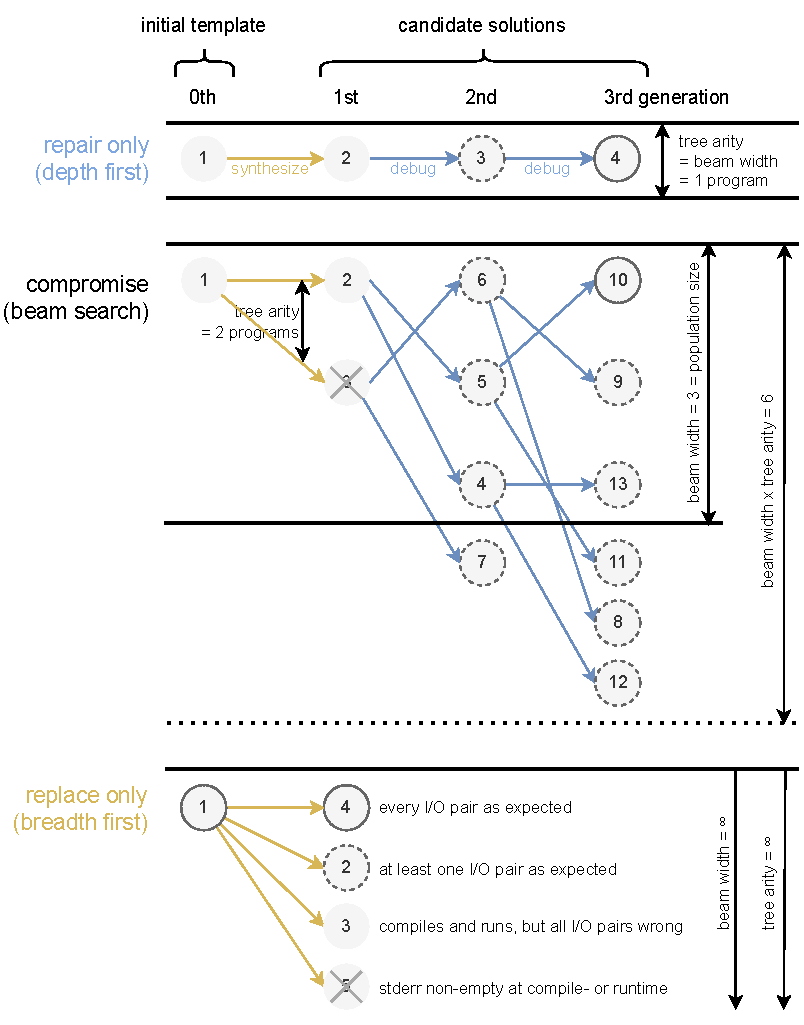
\includegraphics[width=0.6\linewidth, trim={0mm 4mm 0mm 0mm}]{beamsearch.pdf}
    \caption{Repair-replace trade-off as a tree search problem.}
    \label{fig:beam-search}
    % \vspace*{-4ex}
\end{figure}

After evaluating a given candidate solution in \execute{}, \method{} supports two approaches to addressing the candidate's flaws:
\begin{itemize}
  \item \emph{Replace} the candidate with another sample from the current population.
  \item Use \instruct{} and \debug{} to repair the candidate.
\end{itemize}
We refer to this problem as the \emph{repair-replace trade-off}, by analogy with production economics~\cite{jack2000:optimal}. 

How does the choice of hyperparameters $\treearity{},$ the total number of candidate programs in each generation, and $\beamwidth{},$ the number of selected repairs to be preserved in a generation, influence the flow of \method{}?
$\treearity$ and $\beamwidth{}$ act as upper bounds on the \emph{replace} option by limiting the size of the population.
In the edge cases, $\treearity{} = \beamwidth{} = 1$ corresponds to a repair-only process, while $\treearity{} = \beamwidth{} = \infty$ corresponds to replace-only, as illustrated in figure~\ref{fig:beam-search}. 
Note that $\treearity{}$ is defined by $\treearitydraft{}$ for the initial draft solutions in the first generation and $\treearityexplain{} \cdot \treearitydebug{}$ for later generations. 

Observe that a mutation-only genetic algorithm with population size $\beamwidth{},$ such as \method{}, is equivalent to \emph{local beam search} with beam width $\beamwidth{}$ on an $\treearity{}$-ary tree ~\cite[Section 4.1.4]{russell2010:artificial}. This corresponds to a known property of local beam search: it degenerates into depth-first search when $\beamwidth{} = 1$, whereas setting $\beamwidth{} = \infty$ yields breadth-first search.

% Hence, we refer to $\treearity{}$ as \emph{tree arity} and $\beamwidth{}$ as \emph{beam width}.

\section{Related Work}
\label{sec:related-work}

Until recently, the tasks of program synthesis \cite{gulwaniProgramSynthesis2017} and program repair \cite{gouesAutomatedProgramRepair2019, petke2018:genetic} have been considered separately.
However, a number of important studies bridging this gap in the application of Large Language Models have been carried out concurrently with this work, listed below.

\cite{fanAutomatedRepairPrograms2023} incorporate a program repair step into a program synthesis pipeline where the initial synthesis is done by the Codex model \cite{chen2021:evaluating} and for program repair both Codex and state of the art specialized repair tools such as TBar and Recoder \cite{Defects4JDatabaseExisting} are considered and compared. \cite{zhangSelfEditFaultAwareCode2023} do the same, but fine-tune PyCodeGPT-110M \cite{zanCERTContinualPretraining2022} to use it as a repair model. The resulting framework is a two-step process (1 draft step and 1 debug step), while iterative evolution and search are not explored. 

Evolution through Large Models (ELM) \cite{lehmanEvolutionLargeModels2022} proposes using a language model in place of a mutation operator within a traditional genetic programming framework \cite{koza1994:genetic}. They use an type of instruction fine-tuned model trained on git commit messages known as a diff model \cite{DiffModelsNew2023}. However, the model is not directed to solve the programming problem at hand nor to fix bugs, instead, it is provided with generic instructions such as "Change function f". This approach is meant for fields where creative open-endedness~\cite{stanleyWhyGreatnessCannot2015a}, rather then satisfying concrete requirements, is encouraged.

\cite{dongSelfcollaborationCodeGeneration2023} are guided by the metaphor of a multi-agent conversation: their program synthesis loop begins with an analyst LLM generating a plan in natural language, a coder LLM executing it and a tester LLM giving feedback. They implement a repair-only approach and their \execute{} agent is a language model that predicts the output of a program without compilation and/or execution - an instance of chain-of-thought prompting \cite{yuBetterChainofThoughtPrompting2023} for program synthesis.

\cite{jiangSelfEvolveCodeEvolution2023} is a repair-only version of SEIDR that demonstrates the benefits of LLMs evolving not just the source code, but an additional natural language text file that acts as the system's knowledge base, to be included in the model prompt when generating code.

\cite{xiaConversationalAutomatedProgram2023,chenTeachingLargeLanguage2023,shinnReflexionLanguageAgents2023} explore an iterative approach to program synthesis not unlike SEIDR. However, they do not explore the repair-replace tradeoff and exclusively implement the repair-only approach that is prone to local minima.

Finally, Self-Taught Optimizer (STOP) \cite{zelikmanSelfTaughtOptimizerSTOP2023} takes the concept of self-improvement to the next (delightfully meta) level and uses a large language model to edit the evolutionary algorithm itself (i.e. fig. \ref{fig:method}). See their section 8 for reflections on AI Safety.

\section{Expermental Setup}
\label{sec:eval}

To explore the capabilities of \method{} and its generalisability, we test the framework on two benchmarks  with varied search strategies and use two programming languages. 
The problems in the benchmarks originate from coding competitions and human-written programming assignments. 
During our empirical evaluation of \method{} performance, we address the following research questions:
\head{RQ1. Repair-replace trade-off exploration} 
What is the impact of using different tree search strategies
in the autonomous programming setting? 
We experiment with six different tree arities for the quality-based ranking and study their impact on the number of resolved problems as well as the speed of obtaining solutions.
\head{RQ2. Quality-diversity vs. average quality-first based ranking} 
How does the quality-diversity ranking strategy impact the performance in comparison to average quality-first ranking strategy? 
We run experiments with lexicase selection as the ranking strategy and four non-corner case tree arities.
\head{RQ3. Generalisability of the approach to different LLMs} 
How does the choice of an LLM affect the performance of SEIDR? 
We choose the best performing combination of hyperparameters, i.e., a tree arity and a ranking strategy, for experiments with other LLMs and compare the results with previous work obtained without \method{}. 


\subsection{Data}
\label{sec:data}

Our experiments use the Program Synthesis Benchmark~2 (PSB2)~\cite{helmuth2022:applying} and HumanEval-X~\cite{zheng2023:codegeex} in C++ and Python. 
The key criteria for the benchmarks choice are availability task descriptions in English and unit tests in Python and C++ or language-agnostic unit tests. 
We focus on the widely used benchmarks in the areas of generative LLMs and genetic programming. 

\subsubsection{PSB2}
The first dataset is a benchmark suite of 25 problems for program synthesis that resemble small real-world tasks. PSB2 was developed as a more realistic and challenging version of PSB1~\cite{helmuth2015:general}, the latter consisting of textbook problems and is widely used in genetic programming~\cite{sobania2022:choose}. 
The problems require different data structures and control flows to be used for effective solutions and are taken from sources, such as competitive programming platforms and educational courses. 
The problems have descriptions in English, as well as 1 million~(M) tests for training and 1M testing-stage tests, including edge or corner cases that test the resulting program on complicated inputs. 
The tests are provided as I/O pairs and are distributed together with the problem descriptions as a PyPI package.\footnote{~\url{https://pypi.org/project/psb2/}} 

In PSB1, the training set consists of the edge test cases and is augmented by random test cases if the number of edge tests is not enough. The test set is formed by random test cases. 
This terminology is preserved in PSB2. 
However, we do not have a training or fine-tuning phase in our experiments, because the models are not made available for further training. Instead, we validate the framework with an existing pre-trained LLM for code and text as its parts. 
Therefore, we only have the validation and test phases. 
We will refer to training test cases in the PSB terminology as validation test cases in this study. 

\subsubsection{HumanEval-X}
The second dataset we use is a development from the original set of human-written programming tasks in HumanEval~\cite{chen2021:evaluating}, which a standard code generation benchmark for LLMs.
HumanEval consists of 164 problems with a docstring representing problem description, a function signature, a correct solution and unit tests in Python. 
HumanEval-X is a result of translation of correct programs and unit tests to five programming languages. 
We use HumanEval-Python for experiments in Python to ensure comparison with other models in the setup without \method{}. 
In addition, we test \method{} on the HumanEval-C++ part of HumanEval-X to compare with results obtained on PSB2. %here and in an earlier \method{} study~\cite{liventsev2023:fully}. 

The test functions of HumanEval-X contain all tests in one function. We split the aggregated test functions into separate tests so that the \rank{} agent can evaluate the \text{score}. 
On average, the number of tests in HumanEval-Python is 7.25 and 6.95 in HumanEval-C++, which is appointed to a repeated additional test present in some HumanEval-Python examples of the following type: \texttt{assert True, "This prints if this assert fails 1 (good for debugging!)"}.
This test type is not present in HumanEval-C++.
To reiterate, we keep the original HumanEval-Python setup for direct comparison with models tested on this benchmark without \method{}. 
Because of the limited number of tests, we pass up to five tests to the draft prompt and make all tests visible to \method{} for the debugging loop. 
In other words, we do not have a held-out test split for HumanEval-X in the same manner as we have it for PSB2.


\subsection{Models}
\label{sec:models}

\method{} uses three LLMs, \synthmodel{}, \textmodel{}, and \debugmodel{} in \synthesize{}, \instruct{}, and \debug{}, correspondingly. 
These models can be instantiated with the same LLM or different ones. 
The main pre-requisite is that \synthmodel{} and \debug{} are a text-to-code models which take both a textual description and a draft code as input.
Therefore, \synthmodel{} and \debug{} can be a chat model, a code completion model, an instruction fine-tuned or a foundation generative language model pre-trained on code in addition to text. 
By analogy, the text-to-text \textmodel{} can be a chat, instruction fine-tuned, a text completion or generation model pre-trained on text and code.
In our experiments, all three models are instantiated with the same fixed model. 

We use the OpenAI Generative Pre-trained Transformer \texttt{gpt-3.5-turbo}\footnote{\url{https://platform.openai.com/docs/model-index-for-researchers}}  for the experiments with repair-replace trade-off exploration (RQ1) and experiments with quality-diversity and average quality-first ranking strategies (RQ2). 
The GPT-3.5 model is an improvement over the GPT-3~\cite{brown2020:language} 175B-parameter model optimized for chat available via an API.
GPT models are auto-regressive transformer models which have the decoder-only architecture as opposed to the original full encoder-decoder transformer.
They are pre-trained on both text and code and excel at sequence-to-sequence generative tasks, including code-to-code, text-to-code, and code-to-text.

To evaluate generalization capabilities of \method{} on the chosen benchmarks, we have chosen an open-source competitor of GPT models, Code Llama Instruct 34B~\cite{roziereCodeLlamaOpen2023}. 
This model is an advancement on the Llama 2 model~\cite{touvron2023:llama}, an auto-regressive transformer model fine-tuned for code infilling (cloze-style generation), processing longer context windows and instructions.
This model is run as an with the best performing set of hyperparameters found for GPT-3.5 on each of the benchmarks in C++ and Python.
We also compare the performance of \method{} with the current state-of-the-art without \method{} as reported in the corresponding studies (see Section~\ref{sec:results-rq3}).

\subsection{Prompts}
\label{sec:prompts}

Our implementation is optimized for instruction and chat models, which use prompts as inputs represented as text, partially with code fragments.
The models use a system message which describes the ``role'' of the LLM and a regular message that works as an instruction or a chat message from a user.
To provide more context, we always use a problem description, problem name, programming language to the model as textual input (\texttt{descr}). 
As code, we also add an initial template depicted in figure~\ref{fig:template} to \synthmodel{} and the current program candidate to \textmodel{} and \debugmodel{}.

The resulting prompts are as follows.
System message is: 

\begin{lstlisting}
You are an experienced software developer. You write concise code in \{language\}.
The code must read input from user and return output corresponding to the task description.
\end{lstlisting}

Input to \synthmodel{} looks as follows:

\begin{lstlisting}
Solve the following code contest problem: \{problem\_name\}. 
Problem description: \{problem\_description\}.
\{program\_template\}
Only complete the code, do not add triple quotes, do not give explanations.
\end{lstlisting}

Bug explanations are generated with \textmodel{} using the following instructions:

\begin{lstlisting}
  I'm trying to solve the following code contest problem: \{problem\_name\}. 
Problem description: \{problem\_description\}.
Currently, the code is 
\`{}\`{}\`{}
\{program\_candidate\}
\`{}\`{}\`{}
The issue is 
\{stderr or "it must return \{expected\_output\} for input \{input\}, but it returns \{output\}".
Describe how I should fix the code in a very concise manner.
\end{lstlisting}

Debugging model \debugmodel{} operates on the following instruction:

\begin{lstlisting}
Solve the following code contest problem: \{problem\_name\}.
Problem description: \{problem\_description\}.
Currently, the code is 
\`{}\`{}\`{}
\{program\_candidate\}
\`{}\`{}\`{}.
Modify the code as \{bug\_summary\}.
You must only return correct code. Remove any triple quotes, language name or explanations.
\end{lstlisting}


\subsection{Repair-replace Trade-off Settings}
\label{sec:trade-off-settings}

As described in Section~\ref{sec:beam-search}, the choice of beam width $\beamwidth{}$ and tree arity $\treearity{}$ define the repair-replace trade-off where higher $\beamwidth{}$ and $\treearity{}$ prioritize to repair over replace. 
In the meantime, each of the three LLMs can generate sequences in batches. 
We generate $\treearitydraft{}$ programs in the first generation with \synthmodel{}, $\treearityexplain{}$ bug explanations with \textmodel{} for each program in the first generation, and $\treearitydebug{}$ candidate repairs for each of the debugging instructions using \debugmodel{}.
A new generation of $\treearityexplain{} \cdot \treearitydebug{}$ programs is ranked and filtered to keep the best performing $\beamwidth{}$ candidate programs for generating the next candidates. 

To balance between a reasonable number of experiments and diverse sets of hyperparameters, we fix $\treearityexplain{}=2$ to moderately vary the bug descriptions and set $\treearitydraft{} = \treearitydebug{}.$
The upper limit for the total number of generated program candidates is set to 100 to limit the experimentation time. 
We evaluate six options for these hyperparameters as shown in table~\ref{tab:w-n} in the experiments with average quality-first ranking and four non-corner case options for quality-diversity ranking with lexicase selection. 
The choice of these tree branching hyperparameters and the maximum number of generated programs is motivated by the earlier study, where the best results were obtained for $\treearity{}=10,$ so we explore the area around this value more closely.
In the same study, the majority of problems in PSB2 were solved within the set of first 100 generated programs. Note that the setting $\treearitydraft{}=\beamwidth{}=\infty$ ensures that a second generation of programs does not exist.

\begin{table}
    \centering
    \caption{Tree search hyperparameters.}\small
    \label{tab:w-n}\vspace*{-4mm}
    \begin{tabular}{rcccccc}
    \toprule
    experiment & 1 & 2 & 3 & 4 & 5 & 6 \\
    \midrule
     beam width, $\beamwidth{}$ & 1 & 4 & 8 & 10 & 16 & $\infty$ (100) \\
     \# programs in the 1st generation, $\treearitydraft{}$ & 1 & 4 & 8 & 10 & 16 & $\infty$ (100) \\
     \# bug explanations for candidate, $\treearityexplain{}$ & 2 & 2 & 2 & 2 & 2 & - \\
     \# repairs for each explanation, $\treearitydebug{}$ & 1 & 4 & 8 & 10 & 16 & - \\
     \midrule
     used in quality-diversity ranking & 
     no & yes & yes & yes & yes & no \\
     used in average quality-first ranking  & 
     yes & yes & yes & yes & yes & yes \\
     \bottomrule
    \end{tabular}
\end{table}



\subsection{Performance Indicators}
\label{sec:metrics}

\sloppy %
In our experiments, we compare 
the number of fully solved programs obtained using \method{} with different values of hyper-parameters. 
For a more detailed analysis of results, we use \emph{test pass rate (TPR)} and \emph{Excess Programs Generated (EPG)}.
TPR reflects the percentage of fully passed test cases based on the exact match of program output and test output. 
The TPR metric is used for the final evaluation of generated programs and does not reflect partial passing of the I/O test as opposed to the \emph{score} as calculated by the \rank{} agent. 
To compare our results with recent LLMs, we use \emph{pass@k} metric that shows how many problems have $TPR=1$ if we cut off the tree after generating $k$ programs. 

\debug{} and \execute{} agents generate a number of programs that are replaced or repaired during the search for solution program. 
The number of programs generated before the first occurrence of the program that passes all validation test cases is referred to as EPG. 
EPG is indicative of the computational cost of solving a problem distributed in terms of LLM inferences and program compilations and executions.

\subsection{Implementation Details}
\label{sec:implementation}

To operate with the chosen LLMs in \method{}, we use ollama\footnote{\url{https://ollama.ai/}} and LangChain.\footnote{\url{https://www.langchain.com/}}  
To ensure that the program candidates generated from the same parent program are different from each other, we change the temperature parameter of LLMs. 


Due to repetitive calls to \execute{}, we have to resolve the speed of testing versus precision trade-off while choosing the number of validation test pairs.
We resolve the trade-off by fixing the validation set size at~100. Due to a small number of tests in HumanEval-X, all tests are made visible during the validation step. 
We use 2000 I/O pairs from the test split of PSB2 to evaluate the candidate program that has passed all the validation test cases during debugging. 

In all the experiments, we set the limit to generate a maximum of 100 program candidates during the search of the candidate that passes all validation tests. 
If we reach 100 candidates and none of them passes all validation tests, we report the test pass rate for the last generated candidate. 

\section{Results and Discussion}
\label{sec:results}

In this section, we present combined results for the replace-repair trade-off and ranking approaches and discuss them in the dedicated sections. 
Specifically, we count the number of fully solved problems or tasks as measured by $TPR=1$ in experiments with the settings described in table~\ref{tab:w-n} and present the language-specific results for PSB2 and HumanEval in the figure below:

\begin{figure}[H]
 %
\begin{subfigure}{\linewidth}
\centering
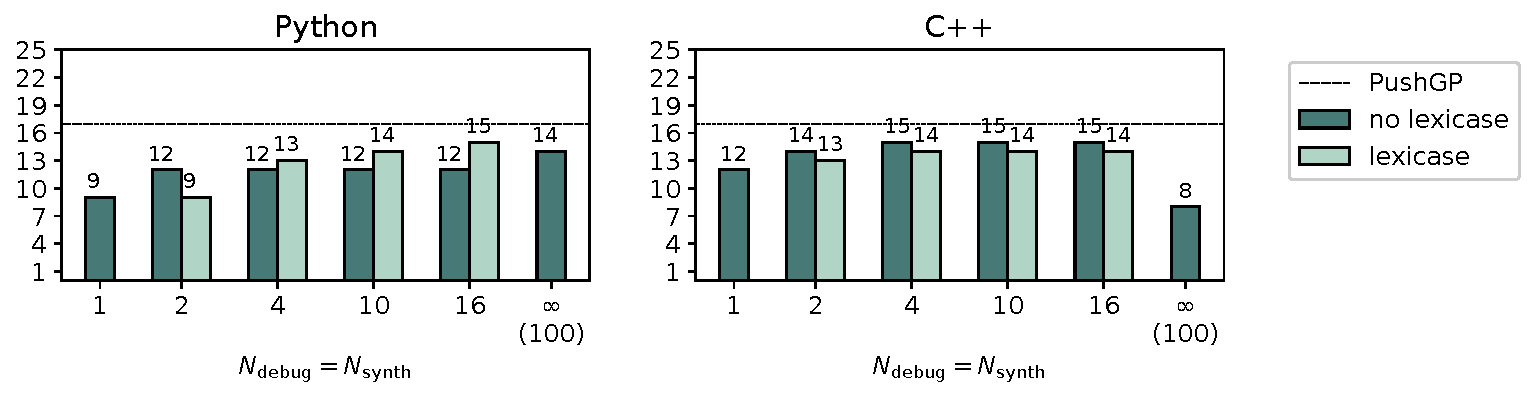
\includegraphics[width=\linewidth, trim={0mm 4mm 0mm 0mm}]{num_solved_problems_vs_bf_psb2_gpt35_01.pdf}
  \caption{PSB2.}
  \label{fig:psb2-gpt3.5}
\end{subfigure}
% \vspace{2mm}
\begin{subfigure}{\columnwidth}
\centering
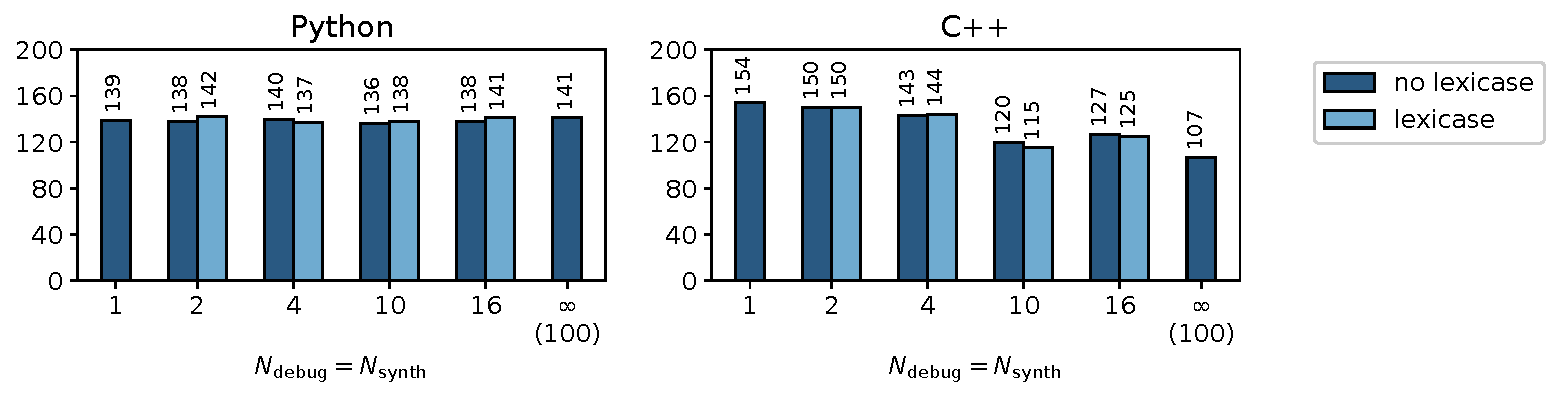
\includegraphics[width=\linewidth, trim={0mm 4mm 0mm 0mm}]{num_solved_problems_vs_bf_humaneval_gpt35_01.pdf}
  \caption{HumanEval}
  \label{fig:he-gpt3.5}
\end{subfigure}
% \vspace{-2mm}
\caption{Repair-replace trade-off with GPT3.5}
\label{fig:repair-replace-trade-off-gpt3.5}

\end{figure}

The figure demonstrates the total number of solved problems as measured by $TPR=1$ using \method{} with GPT-3.5 for the experiments with different numbers of generated programs per instruction ($\treearitydraft$ and $\treearitydebug{}$) and ranking types.

We also explore the speed of obtaining each individual solution with the same experiment settings and report them for PSB2 in figure~\ref{fig:epg-psb2}, HumanEval-Python and HumanEval-C++ in figures~\ref{fig:epg-humaneval-python} and~\ref{fig:epg-humaneval-c++}, correspondingly.
Other experiment-specific graphs and tables are described in the dedicated sections. 


\subsection{RQ1. Repair-replace Trade-off Exploration}
\label{sec:rq1}

We compare the number of solved problems in the experiments with $\treearitydraft{}=\treearitydebug{}$ values of 1, 2, 4, 10, 16, $\infty$ (100) and $\treearityexplain{}=2$ in Python and C++ in figure~\ref{fig:repair-replace-trade-off-gpt3.5}. 
We will refer to the (equally set) values of $\treearitydraft{}$ and $\treearitydebug{}$ as $N^*$ further in the text.
The results of \method{} are compared to the baseline performance of PushGP on the PSB2 benchmark, which solves 17 out of 25 problems. 
Note that experiments with $N^*=1$ and $N^*=\infty$ can be considered as ablation studies, where the replace option and repair option is turned off, correspondingly. 

For PSB2, the results highlight the benefit of compromise strategies with tree arity of 2, 4, 10, and 16 over repair-only ($N^*=1$) and replace-only ($N^*=\infty$) strategies (see figure~\ref{fig:psb2-gpt3.5}). 
The repair-only scheme is outperformed by other strategies. 
We explain the poor performance of repair-only strategy by the fact that the search space is under-explored. 
Specifically, the replace scenario ensures the LLM for debugging represented by GPT-3.5 in our experiments generates different updates of program candidates using variable temperature.
The probability of finding a better fix is higher when more alternatives are generated to update the draft program at $N^*>1$ compared to $N^*=1$. 
The search strategy with lexicase selection and $N^*=16$ yields the best results on Python and tree arities  $N^*=4, \; 10, \; 16$ with the average quality-first search strategy outperform other tree arities but do not outperform PushGP.
Note that \method{} with Codex (GPT-3 trained on code) as \synthmodel{} and \debugmodel{} and GPT-3 as \textmodel{} does outperform PushGP on Python and performs on par with PushGP in C++ with $N^*=10$ and $\treearityexplain{}=1$. %as described by \cite{liventsev2023:fully}.
This can be explained by the generic chat-tuned nature of GPT-3.5 as opposed to Codex' code-specific pre-training. 
% The results imply that generating a moderate number of programs in parallel during the \debug{} step works better than the policies in which more updates are generated for each program (2-16) or only one program is updated iteratively on the datasets .

For HumanEval-C++, the trend is that the larger number of tasks are solved with smaller tree aritites holds (see figure~\ref{fig:he-gpt3.5}). 
However, the leading tree arity value is $N^*=1,$ which diverges from the PSB2 findings. 
In HumanEval-Python, the best result is obtained with  $N^*=2$ with lexicase selection, while the second best result is observed for $N^*=16$ with lexicase  selection and $N^* = \infty \; (N^*=\text{max programs}=100)$ without lexicase selection.
It is notable that HumanEval-X has less tests than PSB2 which suggests that with more thorough testing, the leading tree arity can be different.

The speed of finding a solution broken down to the problem level is shown in the figures below. Number of Excess Programs Generated are reported in color and test pass rate as numbers depending on the type of debug prompt. Higher EPG values are shown in darker shades than low EPG. We denote solved problems with ``+'' (test pass rate = 1), unsolved problems with ``-'' (test pass rate = 0), and show the test pass rate for partially solved problems.

\begin{figure}[H]
  \centering
  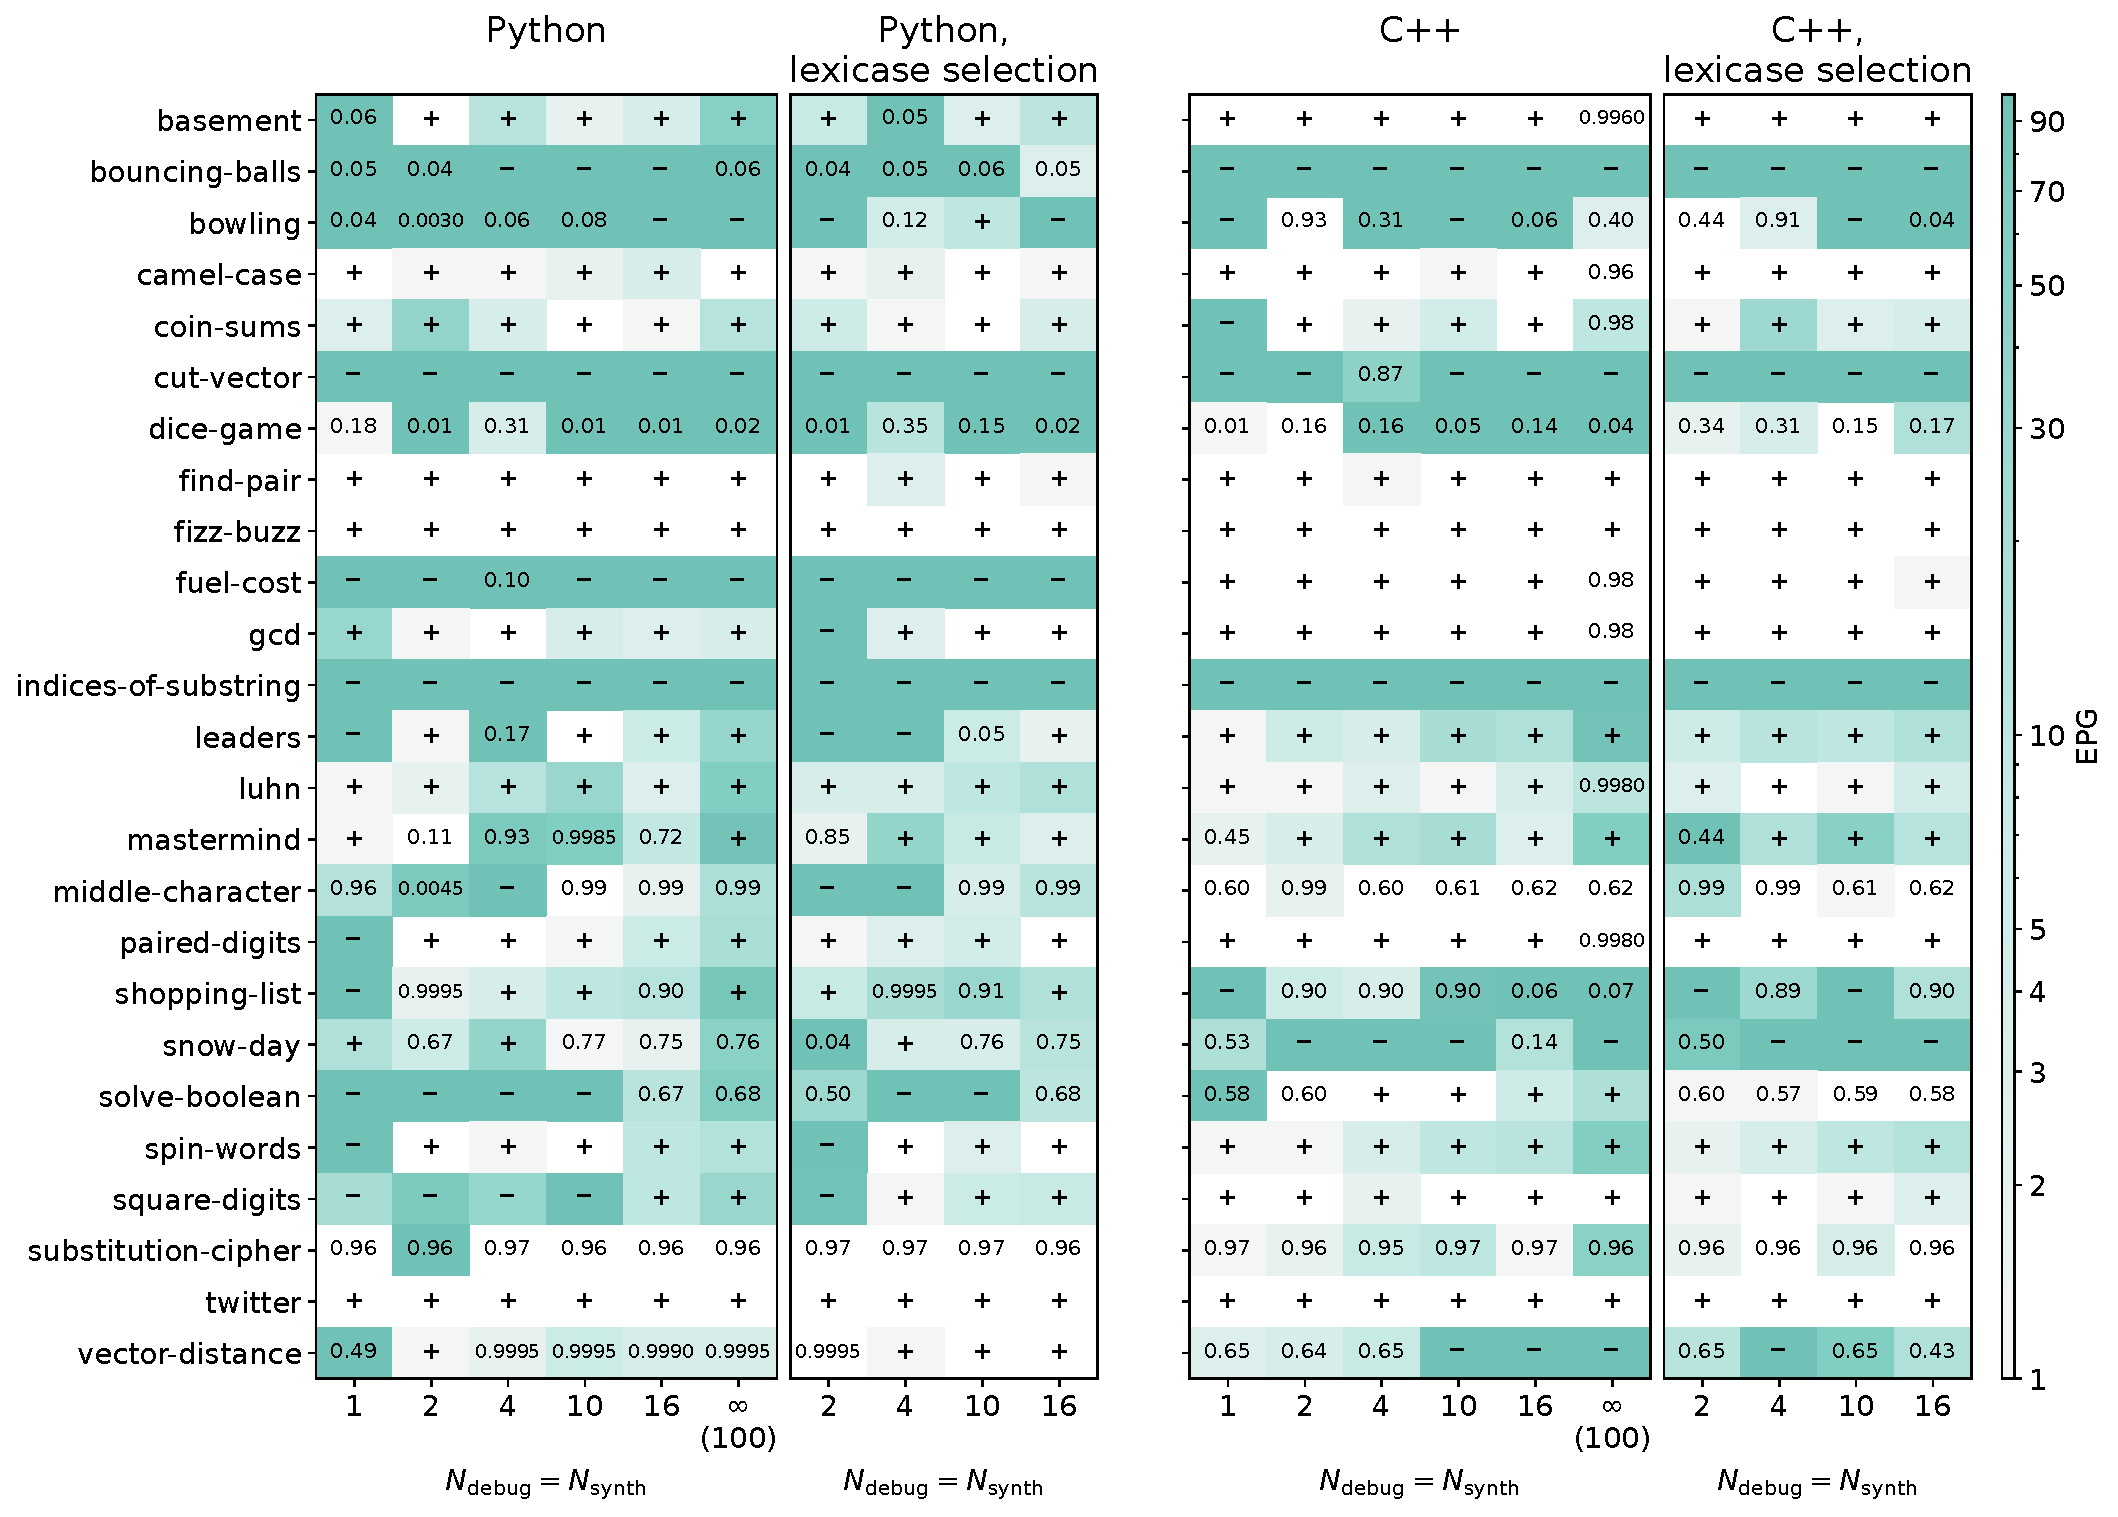
\includegraphics[width=.82\linewidth, trim={0mm 2.8mm 0mm 2mm}, clip]{epg_psb2_gpt35_01.pdf}
  \caption{EPG and Test Pass Rate for PSB2. }
  \label{fig:epg-psb2}
\end{figure}


\begin{figure}[H]
  \centering
  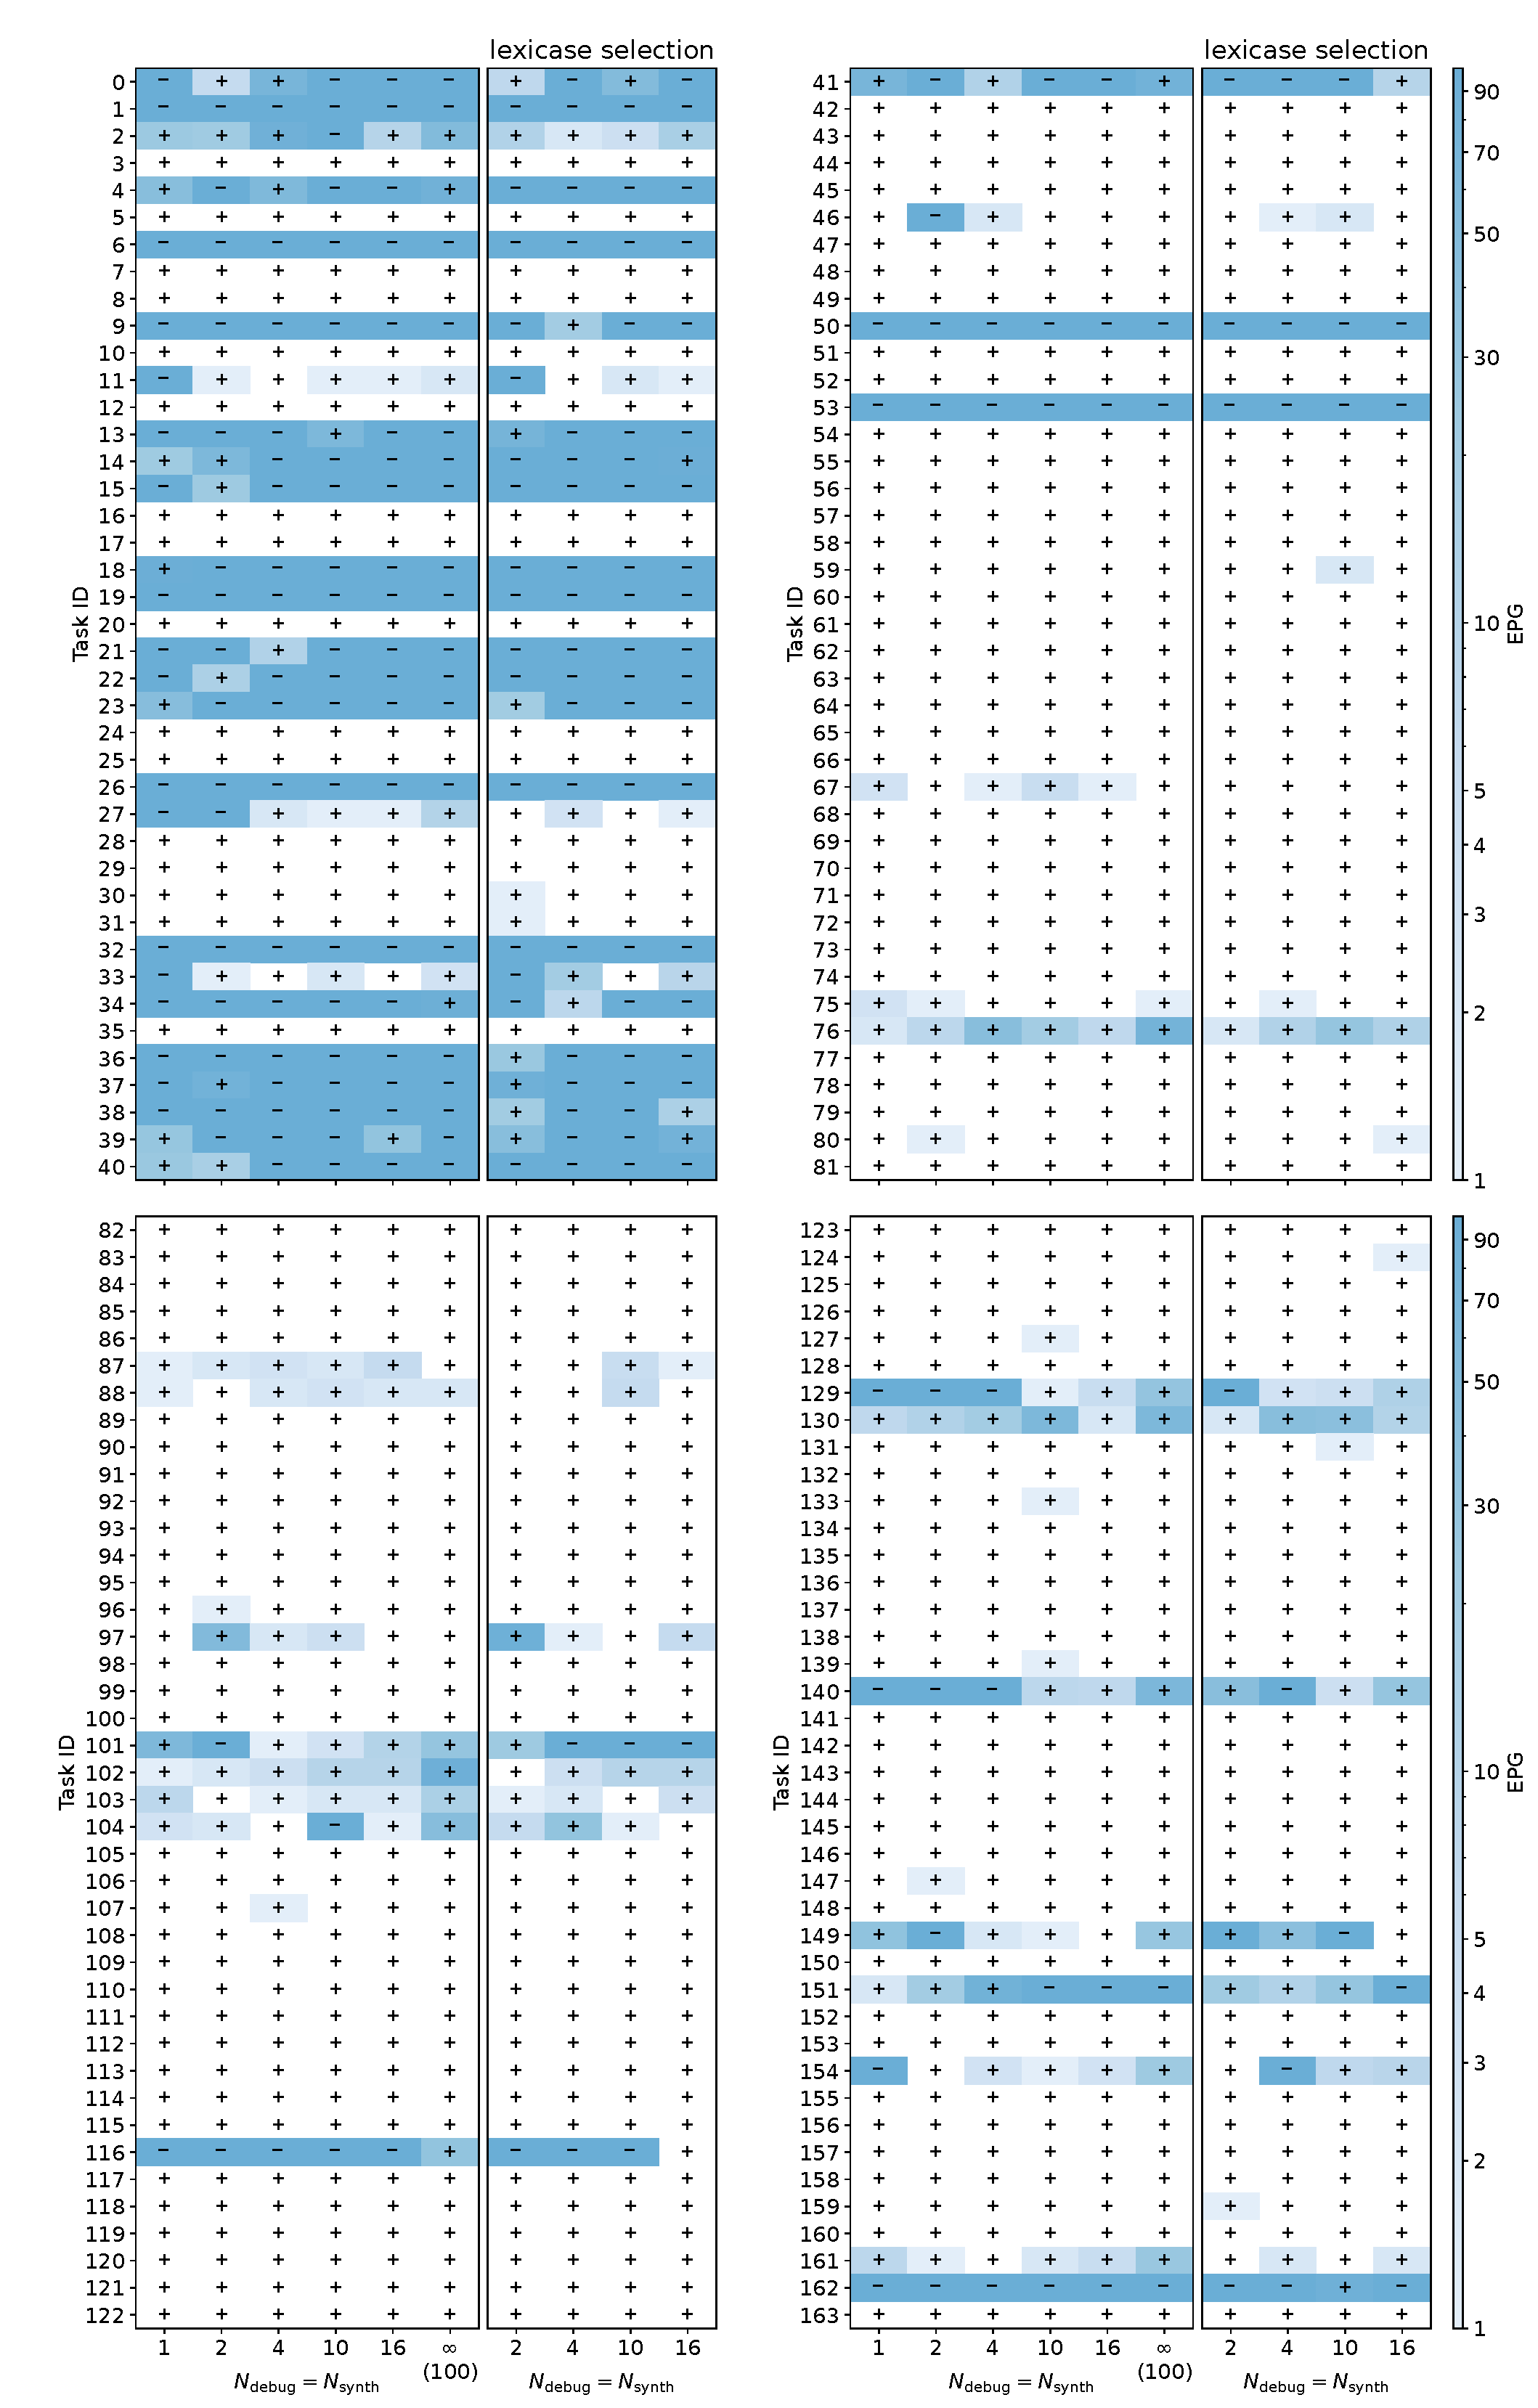
\includegraphics[width=.82\linewidth, trim={0mm 2.8mm 0mm 2mm}, clip]{epg_humaneval_Python_gpt35_01.pdf}
  \caption{HumanEval-Python: Excess Programs Generated and Test Pass Rate.}
  \label{fig:epg-humaneval-python}
\end{figure}

\begin{figure}[H]
  \centering
  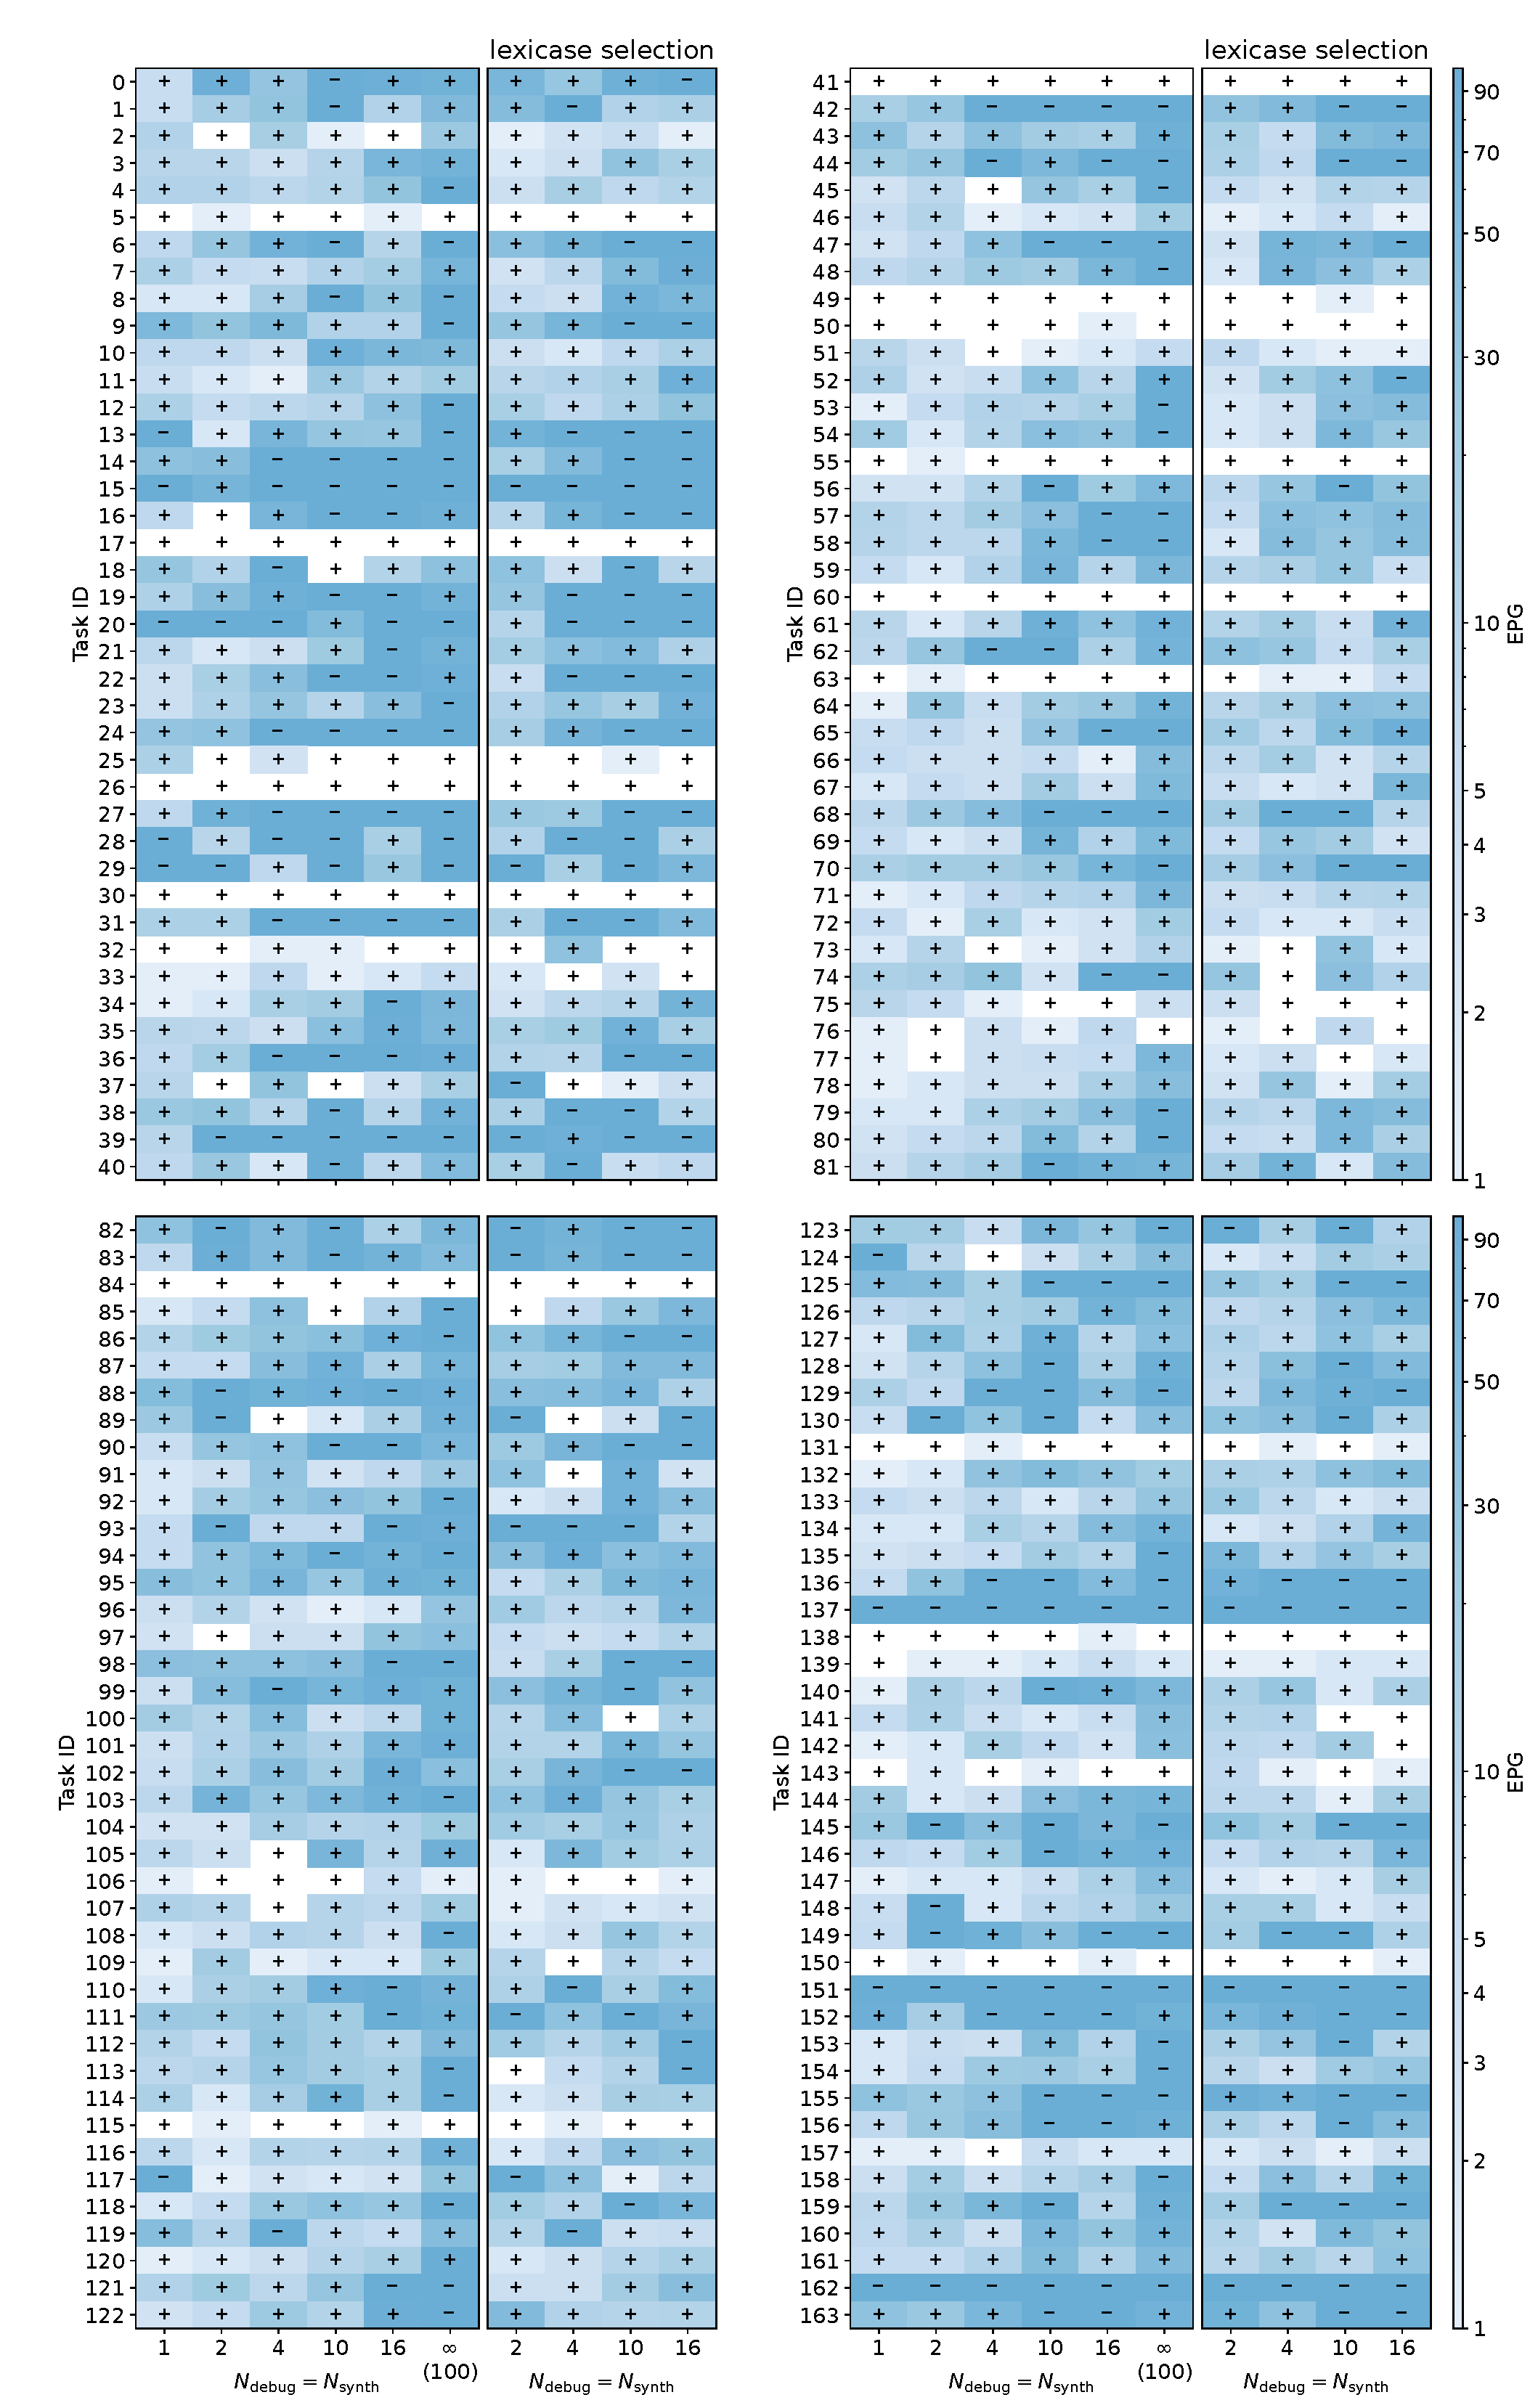
\includegraphics[width=.82\linewidth, trim={0mm 2.8mm 0mm 2mm}, clip]{epg_humaneval_C++_gpt35_01.pdf}  %
  \caption{HumanEval-C++: Excess Programs Generated and Test Pass Rate .}
  \label{fig:epg-humaneval-c++}
\end{figure}

In PSB2, the fastest solutions to all validation sets without lexicase  selection in Python is found using $N^*=16$ (observed in columns with the prevalence of light-colored cells over the dark-colored cells), both with and without lexicase  selection, and in C++  using $N^*=2$, with and without lexicase selection, with a runner-up of $N^*=16$ with lexicase  selection.
Bowling in Python, PSB2, and task 162 in HumanEval-Python experiments are the only problems solved by a unique set of hyperparameters, $N^*=10$ with lexicase selection, and not solved by any other set of hyperparameters.

In HumanEval-Python, for the majority of solved tasks, the solutions are found at the first attempt which negatively influences the analysis of repair-replace trade-off on this dataset, since all tree search algorithms are equivalent when the root node of the tree is the solution.
For HumanEval-Python, task IDs 11, 27, 33, 101-104, 129-130 are solved faster with $N^*=4, \; 10$ with lexicase selection and $N^*=4, \; 10, \; 16$ without lexicase selection more frequently than with other values of $N^*$ (see figure~\ref{fig:epg-humaneval-python}).
The trend of better results with smaller values of $N^*$ is true both for the number of solved problems (figure~\ref{fig:he-gpt3.5}) and higher speed of finding solutions (see figure~\ref{fig:epg-humaneval-c++}) in C++.
% Smaller values of $N^*$ result in both faster and more solutions (without lexicase selection or on par with it) for HumanEval-C++, which is indicated by brighter colors in the columns on the left of the heatmaps compared to the columns on the right.

\begin{highlight}
\textbf{Answer to RQ1:} 
Search strategies in \method{} with tree arity $N^*$ larger than one and lower than $\infty$ benefit from the replace possibility of the \method{} framework as a consequence of using variable temperature for GPT-3.5 on PSB2.
In the experiments, where the majority of problems are solved with more than one attempt, such as HumanEval-C++, lower tree arities (1, 2, 4) yield better results, which indicates the importance of the \debug{} agent in \method{}. 
No single leading tree arity $N^*$ was found for \method{} with GPT-3.5 on PSB2 and HumanEval-X.
\end{highlight}

\subsection{RQ2. Experimenting with Average Quality-first and Quality-diversity Ranking Strategies}
\label{sec:lexicase-results}

Quality-diversity ranking is implemented as lexicase selection and tested with the number of generated programs in the first generation (drafts) and candidates generated from bug explanations (tree arities $N^*=2,\; 4, \; 10, \; 16$) as mentioned in table~\ref{tab:w-n}.
We have partially discussed the results concerning the use of lexicase selection and average quality-first ranking while describing figures~\ref{fig:repair-replace-trade-off-gpt3.5} and~\ref{fig:epg-psb2}-\ref{fig:epg-humaneval-c++}. 
Therefore, in this section, we focus on the cases where lexicase selection-based ranking outperformed average quality-first ranking and the speed of obtaining solutions with lexicase selection and average quality-based ranking.

We present the analogy of the solution speed metric for all tree arity values and fixed default debug instruction in figure~\ref{fig:epg-distribution}. 
In detail, we show the distribution of EPG values in all experiments to explore how many candidate updates are generated before the solution is found.
We zoom in to the cases with solutions found with up to the first 10 program candidates in figures~\ref{fig:psb2-epg-distrib-step-1} and~\ref{fig:humaneval-epg-distrib-step-1} for PSB2 and HumanEval-X, respectively. 
The coarser-grained EPG distribution with the step of 10 candidates is shown in figures~\ref{fig:psb2-epg-distrib-step-10} and~\ref{fig:humaneval-epg-distrib-step-10}. 

% %%%%%%%%%%%%%%%%%%%%%%%%%%%%%%%%%%%%%%%%%%
% % EPG distribution
% %%%%%%%%%%%%%%%%%%%%%%%%%%%%%%%%%%%%%%%%%%
\begin{figure}
 %
\begin{subfigure}{\columnwidth}
\centering
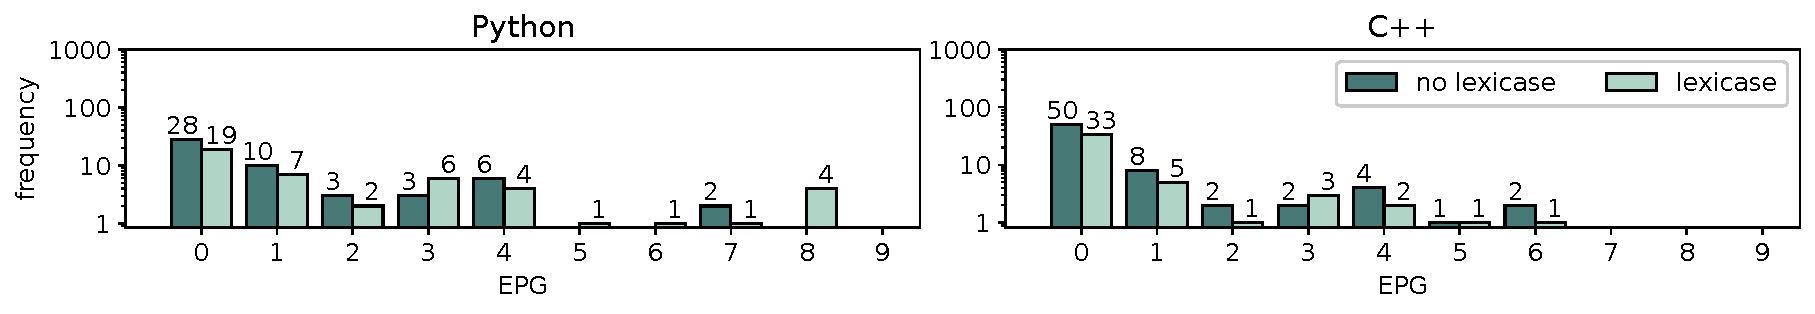
\includegraphics[width=\linewidth, trim={0mm 4mm 0mm 0mm}]{epg_distribution_psb2_gpt35_1_01.pdf}
  \caption{HumanEval: 0 $\leq$ EPG $\leq$ 10 with step 1.}
  \label{fig:psb2-epg-distrib-step-1}
\end{subfigure}
% 
% 
\begin{subfigure}{\columnwidth}
\centering
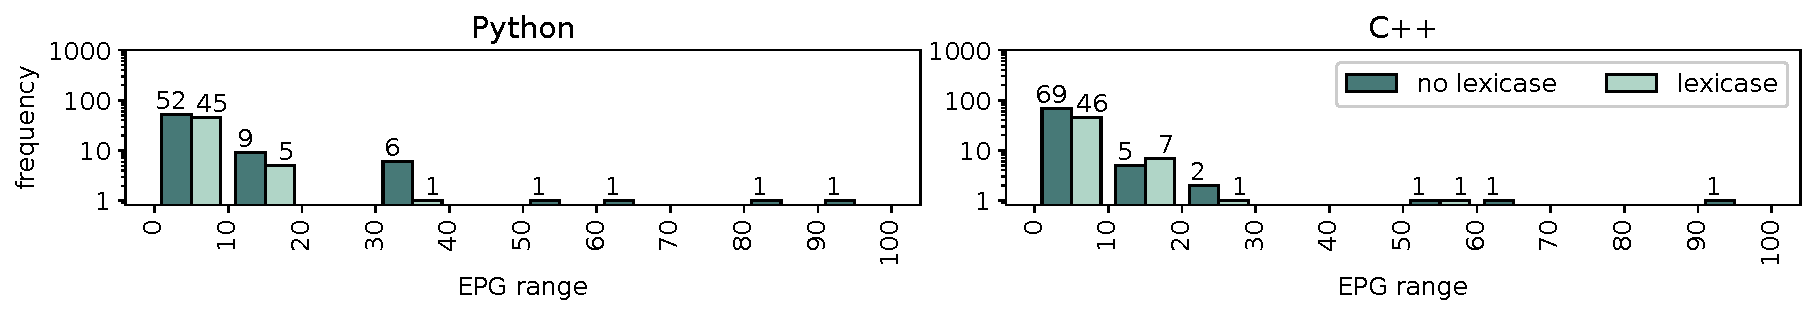
\includegraphics[width=\linewidth, trim={0mm 4mm 0mm 0mm}]{epg_distribution_psb2_gpt35_10_01.pdf}
  \caption{HumanEval: 0 $\leq$ EPG $\leq$ 1000 with step 100.}
  \label{fig:psb2-epg-distrib-step-10}
\end{subfigure}
% 
\begin{subfigure}{\columnwidth}
\centering
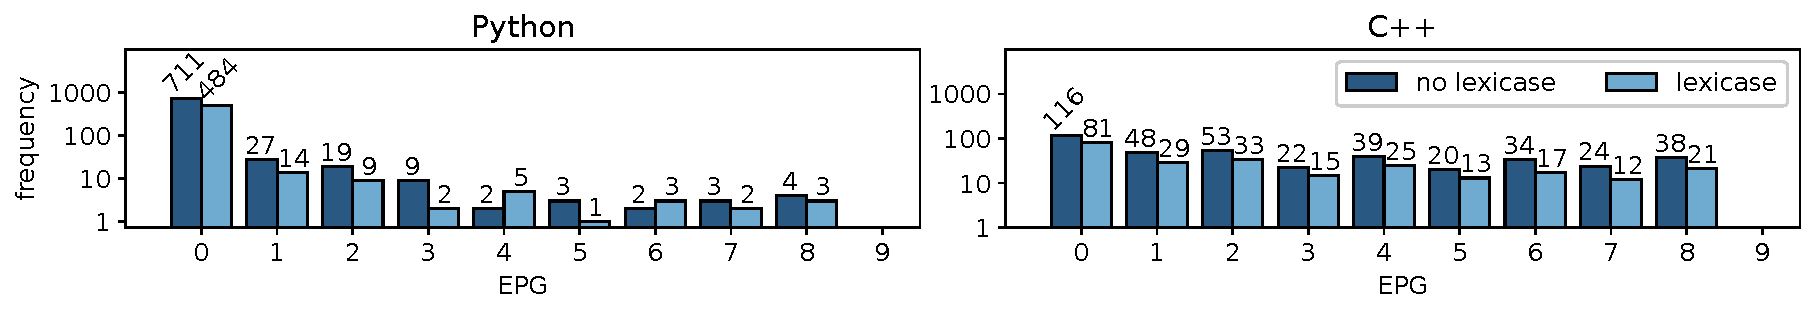
\includegraphics[width=\linewidth, trim={0mm 4mm 0mm 0mm}]{epg_distribution_humaneval_gpt35_1_01.pdf}
  \caption{HumanEval: 0 $\leq$ EPG $\leq$ 10 with step 1.}
  \label{fig:humaneval-epg-distrib-step-1}
\end{subfigure}
% 
\begin{subfigure}{\columnwidth}
\centering
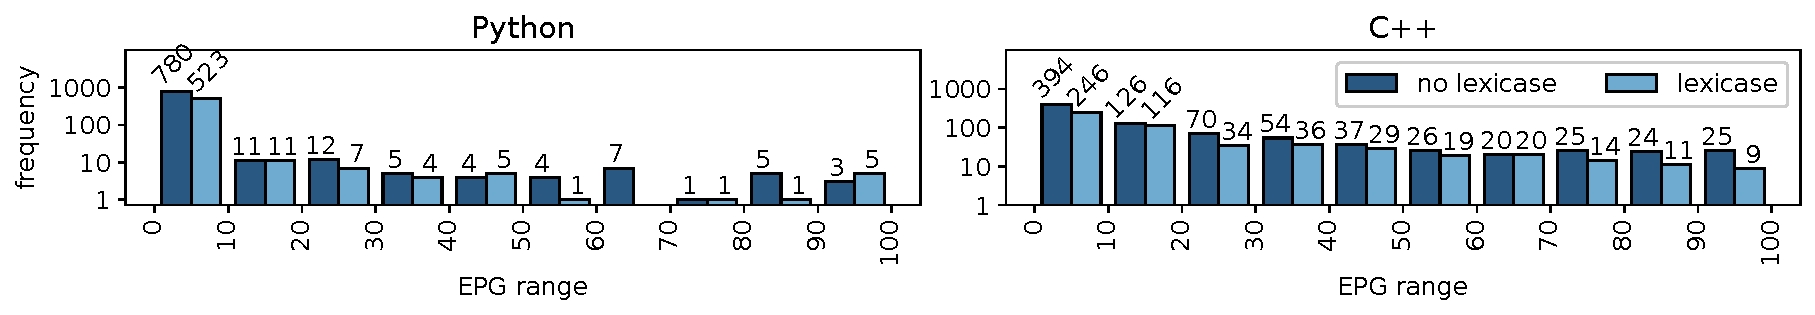
\includegraphics[width=\linewidth, trim={0mm 4mm 0mm 0mm}]{epg_distribution_humaneval_gpt35_10_01.pdf}
  \caption{HumanEval: 0 $\leq$ EPG $\leq$ 1000 with step 100.}
  \label{fig:humaneval-epg-distrib-step-10}
\end{subfigure}
\caption{Number of generated programs during each problem-solving attempt by tree arities $\treearitydraft{}, \; \treearitydebug{},$ }
\label{fig:epg-distribution}
\end{figure}

In the experiments where a solution was found, more runs without lexicase selection obtained $TPR=1$ earlier than the runs with lexicase selection (see figure~\ref{fig:epg-distribution}).
In general, out of 250 experiments for each language for PSB2, in 18.8\% of runs in Python and 33.2\% runs in C++, the draft program is already the solution (EPG=0). 
For 35.2\% of experiments in Python and 44.0\% runs in C++, the solution is found after discarding 5 candidates. 

The majority of experiments do not generate more than 10 programs. 
However, 8 PSB2 problems are solved with more than 50 generated programs in Python and in C++, 4 in each language.
By contrast, in HumanEval-X experiments, the problems are solved faster in Python than in C++, with 72.9\% tasks achieving $TPR=1$ with the draft solution in Python and 12.0\% tasks in C++.
Only 1.7\% experiments in Python reached a solution after discarding 50 candidates, while the analogical measure for C++ is 11.8\%.
Remarkably, although the speed of obtaining solution with $TPR=1$ in C++ is considerably lower, \method{} solved 12 more tasks in C++ (154) than in Python (142). 


% % TODO for extension: Are they the same tasks or different ones? Does seidr solves collectively more than other models or some uniqye problems than other models? 

The EPG distribution results for correctly solved problems with $TPR=1$ imply that the first steps in the update of the draft program are crucial for solving the problem. 
The chances of solving the problem on the later stages of the search are low.
This confirms our initial assumption in Section~\ref{sec:trade-off-settings} that 100 programs are sufficient.

Quality-diversity ranking strategy outperformed the average quality-first ranking in the Python experiments, both on PSB2 ($N^*=4, \;, 10, \; 16$) and HumanEval-Python ($N^*=2, \;, 10, \; 16$). 
To explore the impact of using quality-diversity over average quality-based ranking, we filter out the problems solved with more than one attempt and show the best average score described in Section~\ref{sec:execute} in figure~\ref{fig:avg-score-lexicase} for PSB2 and HumanEval-Python. 
We can see that the majority of problems are solved with a jump of average score from zero to one, except for one case in HumanEval-Python and two cases in PSB2 as shown by two angled lines in figure~\ref{fig:psb2-score-lexicase} and one such line in figure~\ref{fig:humaneval-score-lexicase}. 
These three experiments were the only cases where the ranking strategy worked. 
In other experiments with zero average scores reported up until the moment the solution is found, lexicase selection does not reorder the program candidates, which is also true for the majority of experiments with average quality-based ranking.

%%%%%%%%%%%%%%%%%%%%%%%%%%%%%%%%%%%%%%%%%%
% BEST AVG SCORE FOR LEXICASE IN  PYTHON
%%%%%%%%%%%%%%%%%%%%%%%%%%%%%%%%%%%%%%%%%%
\begin{figure}
 % trim={left lower right upper}
\begin{subfigure}{\textwidth}
\centering
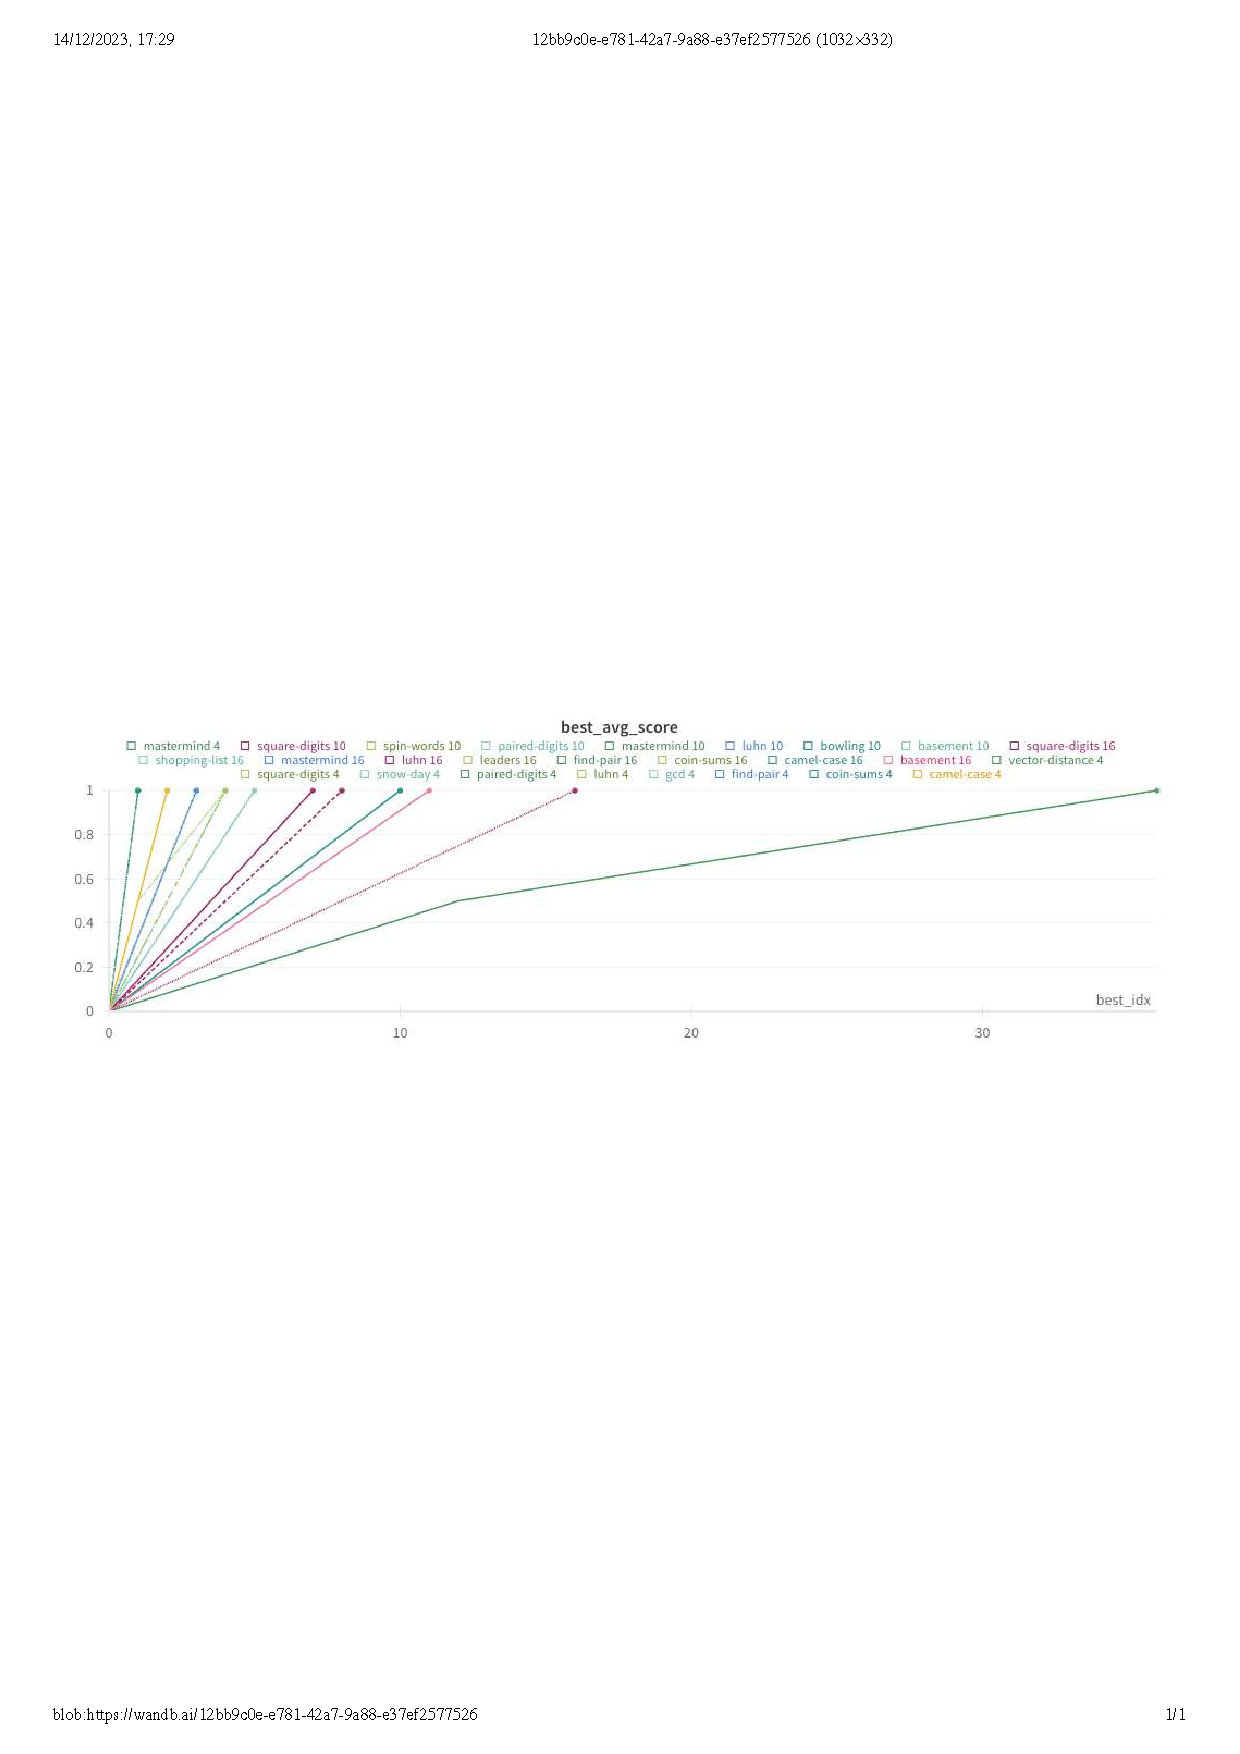
\includegraphics[width=.82\linewidth, trim={0mm 120mm 0mm 133mm}, clip]{lexicase-psb2-2_compressed.pdf}
  \caption{PSB2.}
  \label{fig:psb2-score-lexicase}
\end{subfigure}

% \vspace{2mm}

\begin{subfigure}{\textwidth}
\centering
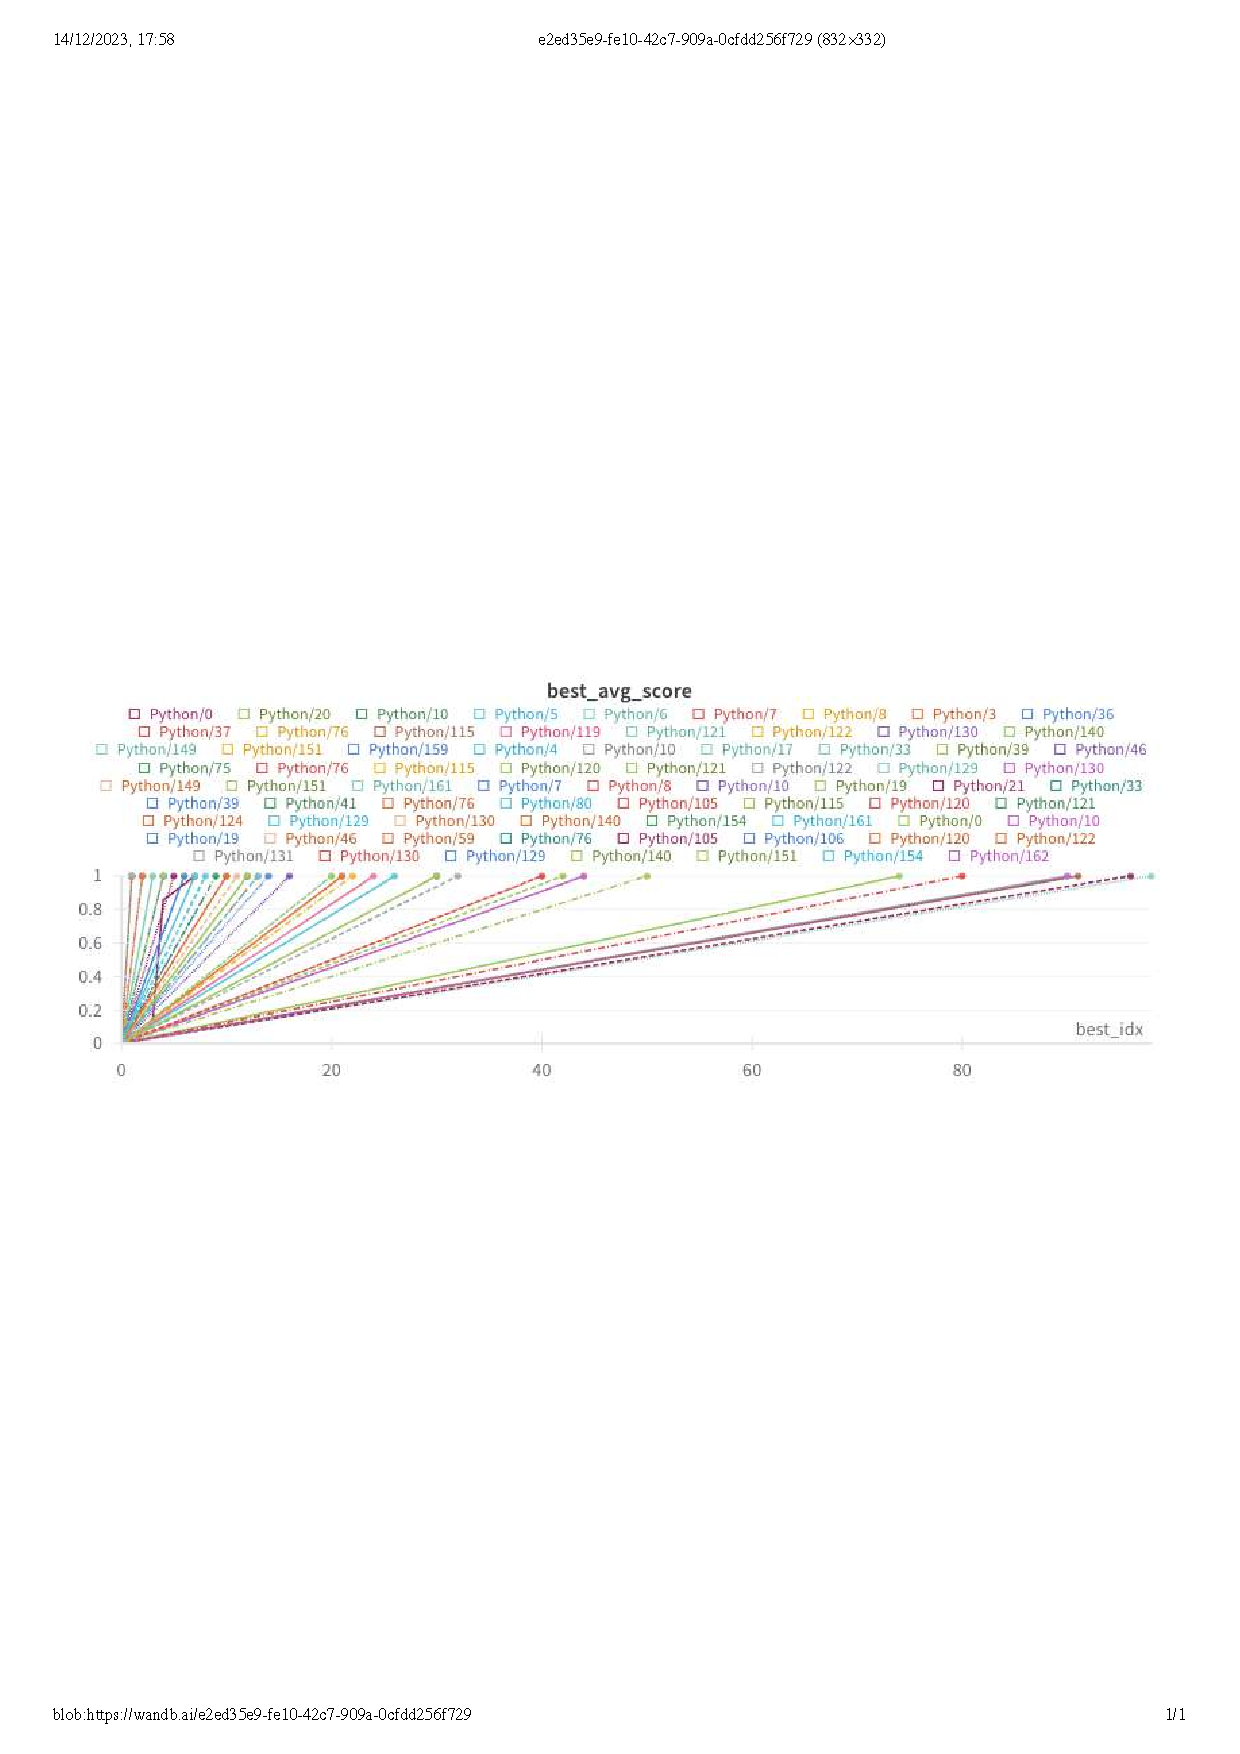
\includegraphics[width=.86\linewidth, trim={0mm 110mm 0mm 147mm}, clip]{lexicase-humaneval-2_compressed.pdf}
  \caption{HumanEval-Python.}
  \label{fig:humaneval-score-lexicase}
\end{subfigure}
% 
\caption{Rolling best average score for problems solved from the second or later attempts with lexicase selection.}
\label{fig:avg-score-lexicase}
% 
\end{figure}


% \begin{mdhighlight}[style=mystyle]
% \vspace*{-1mm}
% \noindent
\begin{highlight}
\textbf{Answer to RQ2: } 
While quality-diversity ranking outperforms average quality-first ranking in several Python experiments, the number of actual reranking steps performed is low. 
No leading ranking strategy is found for \method{} experiments with GPT-3.5 on PSB2 and HumanEval-X in Python and C++.
\end{highlight}
% \end{mdhighlight}
% \vspace*{-2mm}

\subsection{RQ3. Generalisability of \method{}}
\label{sec:results-rq3}

We choose the best performing tree arity for each benchmark and language to run \method{} with Code Llama 34B and compare the results to the findings for GPT-3.5 and Code Llama 34B without \method{} in table~\ref{tab:generalisability-psb2} for PSB2 and table~\ref{tab:generalisability-he} for HumanEval-X. 
The number of problems solved at different cutoffs ($k$) is reported for PSB2 and the percentage of solved problems at different $k$ is shown for HumanEval-X.
We compare the performance of PSB2 solutions synthesized with \method{} to the PushGP genetic programming system with down-sampled lexicase selection~\cite{helmuth2022:problemsolving}. 
For HumanEval-X, we cite the performance of the state-of-the-art models as reported by their authors without \method{}, such as CodeGeex~\cite{zheng2023:codegeex}, GPT-3.5 and GPT-4~\cite{openai2023:gpt4}, for reference, and compare \method{} with GPT-3.5 and CodeLlama results at different cutoffs ($k$ for $pass@k$).

In the PSB2 experiments, \method{} with GPT-3.5 and Code Llama 34B does not outperform \method{} with GPT-3, where Codex was used for code generation and repair steps. 
This finding suggests that using instruction models pre-trained for code generation is a better choice for  \synthesize{} and \debug{} agents of \method{}. 
\method{} with Code Llama performs worse than other models used in \method{} and does not solve any problem in Python. 
Closer inspection into generated candidate programs reveals that the model keeps generating near-misses which resemble correct code but do not pass tests.
Besides, during our experiments with Code Llama 34B loaded to ollama, we have found that the model needs frequent restarts. 

While \method{} with GPT-3.5 and Code Llama 34B does not outperform other state-of-the-art models, \method{} experiments with GPT-3.5 and $N^*<100,$ i.e., using repair steps as well as replacement as opposed to replacement-only evaluation, show consistently better results for GPT-3.5, which is also true for PSB2.  
Importantly, \method{}  with Code Llama 34B outperforms the current state-of-the-art model CodeGeeX, on HumanEval-C++ when comparing pass@10 achieving 77.44\% of solved tasks.
Moreover, \method{} with GPT-3.5 results in higher pass@100 than CodeGeeX: 93.29\% compared to 51.00\%. 

\begin{table}
    \centering
    \caption{Number of solved PSB2 problems using \method{} with different LLMs and PushGP. The best results among \method{}-only experiments at each $k$ are highlighted in bold. The best overall scores are underlined. If pass@100 is not available, the best reported results for a given method are mentioned in brackets.}\small
    \label{tab:generalisability-psb2}\vspace*{-4mm}
\begin{tabular}{llllrrr}
\toprule
Model & Language & $N^*$ & Ranking &  pass@1 &  pass@10 &  pass@100 \\
\midrule
 \method{} w/ GPT-3.5 & Python & 1   & average quality &       4 &        7 &         9 \\
&       & 2   & average quality &       6 &       11 &        12 \\
 &      &     & quality diversity  &       3 &        9 &         9 \\
 &      & 4   & average quality &       5 &        9 &        12 \\
&       &     & quality diversity  &       3 &       \textbf{12} &        13 \\
 &      & 10  & average quality &       6 &       10 &        12 \\
 &      &     & quality diversity  &       \textbf{7} &       \textbf{12} &        14 \\
 &      & 16  & average quality &       3 &       10 &        12 \\
 &      &     & quality diversity  &       6 &       \textbf{12} &        \textbf{15} \\
 &      & 100 & average quality &       4 &        5 &        14 \\
 \midrule
\method{} w/ Code Llama 34B & Python &  16  & quality diversity &    0 &        0 &         0 \\
 \method{} w/ GPT-3 & Python  & 10 & average quality &       - &        - &      (pass@1000=\underline{19}) \\
  \midrule
 PushGP & Python &  -   &    -            &       - &        - &      (\underline{17})\\
\midrule
\method{} GPT-3.5 & C++ & 1   & average quality &       9 &       12 &        12 \\
  &     & 2   & average quality &      \textbf{10} &       \textbf{14} &        14 \\
  &     &     & quality diversity  &       8 &       13 &        13 \\
  &     & 4   & average quality &       8 &       \textbf{14} &        \textbf{15} \\
  &     &     & quality diversity  &      \textbf{10} &       11 &        14 \\
  &     & 10  & average quality &       9 &       12 &        \textbf{15} \\
  &     &     & quality diversity  &       8 &       11 &        14 \\
  &     & 16  & average quality &      \textbf{10} &       13 &        \textbf{15} \\
  &     &     & quality diversity  &       7 &       11 &        14 \\
  &     & 100 & average quality &       4 &        4 &         8 \\
  \midrule
\method{} w/ Code Llama 34B & C++ &  16  & average quality  &    5 &        6 &         8 \\
\method{} w/ GPT-3 & C++  & 10 & average quality &       - &        - &      (pass@1000=\underline{17})\\
\midrule
PushGP & C++ &  -   &    -            &       - &        - &      (\underline{17})\\

\bottomrule
\end{tabular}
\end{table}




\begin{table}
    \centering
    \caption{Percentage of solved tasks for HumanEval-X using \method{} with different LLMs. The best results among \method{}-only experiments at each $k$ are highlighted in bold. The best overall scores are underlined. If pass@100 is not available, the best reported results are mentioned as in the corresponding papers. }\small
    \label{tab:generalisability-he}\vspace*{-4mm}
\begin{tabular}{llllrrr}
\toprule
Model & Language & $N^*$ & Ranking &  pass@1 &  pass@10 &  pass@100 \\
\midrule
\method{} w/ GPT-3.5 & Python & 1   & average quality &   56.71 &    60.37 &     64.02 \\
&        & 2   & average quality &   \textbf{58.54 }&    63.41 &     67.07 \\
&        &     & quality diversity  &   54.27 &    56.71 &     59.15 \\
&        & 4   & average quality &   \textbf{58.54} &    \textbf{65.24} &     \textbf{68.90} \\
&        &     & quality diversity  &   54.88 &    59.76 &     61.59 \\
&        & 10  & average quality &   53.66 &    60.37 &     61.59 \\
&        &     & quality diversity  &   55.49 &    59.76 &     61.59 \\
&        & 16  & average quality &   \textbf{58.54} &    64.63 &     65.85 \\
&        &     & quality diversity  &   54.27 &    60.37 &     63.41 \\
&        & 100 & average quality &   56.10 &    57.32 &     64.02 \\
\midrule
\method{} w/ Code Llama 34 & Python & 4 &  average quality &   34.76 &    49.39 &     54.27 \\
\midrule
Code Llama 34B & Python & - &  - &  48.8  &  76.8   &    93.0 \\
Unnatural Code Llama 34B & Python & - &  - &  62.2  &  \underline{85.2}   &    \underline{95.4} \\
GPT-3.5 (ChatGPT) & Python & - &  - &  48.1  &  -   &    - \\
GPT-4 & Python & -&  - & \underline{67.0}   &  -   &    - \\
CodeGeeX & Python & - &  - &  22.89  &  39.57   &    60.92 \\
\midrule
 \method{} w/ GPT-3.5 & C++ & 1   & average quality &   10.98 &    67.68 &     \underline{\textbf{93.29}} \\
&        & 2   & average quality &   11.59 &    53.05 &     90.85 \\
&        &     & quality diversity  &   11.59 &    46.34 &     87.80 \\
&        & 4   & average quality &   \textbf{14.63} &    43.90 &     87.20 \\
&        &     & quality diversity  &   14.02 &    43.29 &     87.20 \\
&        & 10  & average quality &   12.80 &    31.10 &     73.17 \\
&        &     & quality diversity  &   12.20 &    31.71 &     70.12 \\
&        & 16  & average quality &    9.15 &    28.66 &     77.44 \\
&        &     & quality diversity  &   11.59 &    26.83 &     76.22 \\
&        & 100 & average quality &   10.98 &    14.63 &     64.63 \\
\midrule
\method{} w/ Code Llama 34B & C++ & 1 & average quality &    0.61 &    \underline{\textbf{77.44}} &     85.37 \\
\midrule
Code Llama 34 & C++ & - &  - &  \underline{47.8}  &  -   &    - \\
CodeGeeX & C++ & - &  - &  17.06  &  32.21   &    51.00 \\
\bottomrule
\end{tabular}
\end{table}

% \begin{mdhighlight}[style=mystyle]
% % \vspace*{-1mm}
% \noindent
\begin{highlight}
\textbf{Answer to RQ3:} 
The use of \method{} with GPT-3.5 outperforms the use of GPT-3.5 without \method{}, when the model is called with the same prompts as in \method{}: higher pass@k values are observed with $N^*<100$ than with $N^*=100.$ \method{} with Code Llama and GPT-3.5 does not outperform the current state-of-the-art results methods on PBS2, but does so for HumanEval-C++. 
\end{highlight}
% \end{mdhighlight}
% % \vspace*{-2mm}

\subsection{Threats to Validity}
\label{sec:threats}



External threats to validity concern \method{} performance on different other benchmarks and the use of more language models than the tested ones. 
Specifically, PSB2 and HumanEval-X contain programming tasks which require smaller functions to be generated than production-scale software.
While some canonical solutions provided in HumanEval-Python have been criticised~\cite{liuYourCodeGenerated2023}, we primarily use tests to evaluate the output of \method{}. Therefore, their weaknesses do not impact our results.
% We plan to extend our experiments in future work to explore the generalizability of results to more complex benchmarks.

Internal threats relate to the implementation.
We use PSB2, which has corner case tests in the training set and test regular cases in the test set. 
To ensure a fair comparison with other studies on PSB2, we evaluate and report results on the provided test set of PSB2 which risks that the synthesized programs do not pass some of the training cases. 
Large models for code editing and text completion used in this study are nondeterministic, which impacts results. 
Due to prohibitive model inference costs, each experiment was only run once.
However, our temperature sampling procedure described in section \ref{sec:synth} reduces this stochasticity significantly, especially for low-EPG results.
As with other language models, GPT-3.5 is a black-box model and may generate malicious code~\cite{pearceAsleepKeyboardAssessing2022}. 
The results can be skewed towards high performance in popular programming languages in the pre-training dataset used by authors of the tested LLMs.

\section{Conclusion}
\label{sec:conclusion}
In this study, we propose \method{}: a multi-agent framework to solve the challenge of fully autonomous programming. 
We augment the program synthesis procedure based on the large language models for code generation from templates and textual instructions with a \debug{} agent. 
The \debug{} agent performs tree search across the program candidates generated by a large language model for code.
The LLM used for code repair takes imperfect program candidates and instructions for their improvement as prompts. 
The instructions are obtained from both static templates with failing test case descriptions and templates with auto-generated bug summaries by a text completion language model. 
We explore 11 prompting strategies and the repair-replace trade-off of updating the draft program.

\head{Contributions}
We \method{} with GPT-3.5 and Code Llama 34B as the model for draft program synthesis, explaning errors in synthesized programs and their debugging in Python and C++ on the PSB2 and HumanEval-X benchmarks. 
In our experiments, \method{} does not outperform the state-of-the-art baselines for PSB2 and HumanEval-Python but shows better performance than using LLMs without \method{} with the same prompts as in \method{}.
\method{} achieves the state-of-the-art result for pass@10 (74.44\%) with Code Llama 34B and for pass@100 (93.29\%) with GPT-3.5 on HumanEval-C++. 
The approach requires under 100 program executions to obtain the reported results, 
% in stark contrast to billions\footnote{A problem is considered "solved" by PushGP if at least 1 of 100 runs, each with a limit of 60 million programs, was successful.} of executions in PushGP, 
making it feasible in the areas with costly testing, such as robotics.
Investigation of the repair-replace trade-off shows that \method{} with moderate number of generated programs for each bug explanation is favourable both for obtaining a solution and for the speed of solving a task. 
% Our prompt engineering study shows that bug summaries generated with ``confidence indicators'', such as ``obviously'', improve the performance of \method{} during C++ code synthesis. 
% Overall, our framework shows low performance variability with different prompts, which indicates its robustness.%

\head{Future work}
Further investigation of \method{} generalisability and ranking strategies are some of the areas for future work. 
Benchmarks with more tests than in HumanEval-X may shed more light on the most effective choice of the number of programs generated from each bug explanation, as well as the framework's comparison on large-context projects. 

\vspace*{-1mm}
\section*{Data Availability}
The code and results are attached to the submission and will be made publicly available.

% =======================================================================================
%                                   PART II
% =======================================================================================
\part{For Personal Health}
%----------------------------------------------------------------------------------------
\newpage
\chapter{The Promise} \label{ch:health-motiv}
% Importance of Smart Healthcare
Understaffing has been consistently identified as the major challenge facing Healthcare today \cite{ashleyy.metcalfHospitalUnitUnderstaffing2016,SurveyShowsHidden1993,UnderstaffingSignificantIssue2012,campbell_universal_2013, hudsonUnderstaffing2015, mercerMessageEditorinChief2008, r.stanleyUnderstaffedOverwhelmed2010, munnUnderstaffingWardsCompromising2017, thelancetHealthcareSystemStaffing2018}. Automation tools that make use of Machine Learning (also known as Healthcare 4.0 \cite{tortorellaHealthcareTrendsChallenges2020}) have been consistently identified as crucial for reducing the workload of Healthcare professionals and improving the quality of care \cite{agrawalMachineLearningHealthcare2020, deviDesignImplementationAdvanced2022, g.kumarSurveyMachineLearning2016, ganguliMachineLearningPursuit2020, maityMachineLearningImproved2017, mitraMachineLearningHealthcare2021, pianykhImprovingHealthcareOperations2020, xhaferraRoleMachineLearning2022}. In turn, the shortage of standard benchmarks has been consistently identified as a central roadblock for machine learning in Healthcare \cite{Crown2015Potential, David2020Evaluating, Gu2023Beyond, Harutyunyan2019Multitask, Kathrin2022Benchmark, liventsevEffectivePatientSimulators2021, McDermott2021Reproducibility, Purushotham2018Benchmarking, S2017Benchmark}.

Whether it's ImageNet \cite{dengImagenetLargescaleHierarchical2009} in Computer Vision or GLUE \cite{wangGLUEMultitaskBenchmark2018} in natural language processing, benchmarks are a core research tool in mature applications of machine learning, enabling quantitative analysis of learning methodologies to guide and orient their development.
Machine learning for Healthcare, an emergent field with unique challenges in availability of research datasets \cite{Anshik2021Handling, Gilbert2015market, Pahwa2021Big, Yazhini2019State} lacks an accepted benchmarking standard: recent literature reviews \cite{palMachineLearningHealthcare2023,tortorellaHealthcareTrendsChallenges2020} of the field cover a variety of studies that each use their own (often non-public) benchmark.

The lack of benchmarks is a crucial barrier to advancing the quality and accessibility of care with automatic programming. 
The most promising approach for advancing Healthcare with program synthesis is
\begin{enumerate}
    \item Use clinical data, such as electronic health records, to train a patient simulator: a predictive model of patient’s future health conditional on clinicians’ decisions. 
    \item Use Programmatically Interpretable Reinforcement Learning to search for a program/protocol that performs well in that simulator.
\end{enumerate}

Having developed a sufficiently robust PIRL algorithm, let us now turn our attention to part (1) - effective patient simulators.

%\newpage
%\chapter{The State of the Art} \label{ch:health-sota}
%\section{Existing simulators}
\label{sec:existing}

\subsection{simglucose}
\label{sec:simglucose}

\begin{figure}
    \centering
    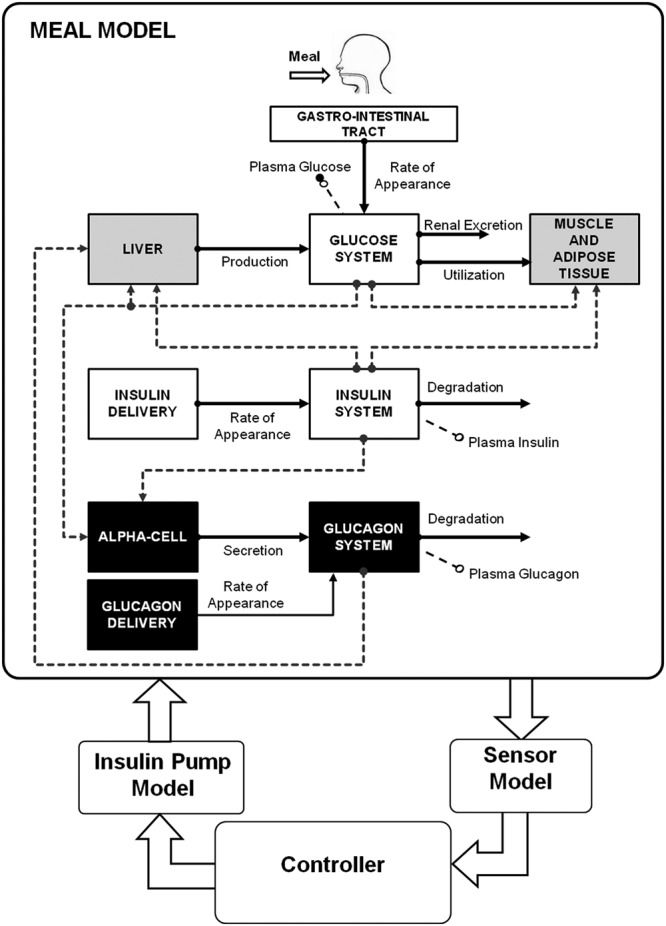
\includegraphics[width=\linewidth]{uvapadova.jpg}
    \caption{UVA/PADOVA equations, visualised}
    \label{fig:uvapadova}
\end{figure}

UVA/Padova \cite{sim-diabetes-fda} is a set of equations used to model type 1 diabetes.
The equations, outlined on figure \ref{fig:uvapadova}, were developed by clinical experts and validated on a dataset of 32 people aged 38 ± 12 years.
It is widely used in Healthcare and even approved in the United States as a replacement for clinical trials.
It provides $p_o(o | s, a)$ and $p_s(s_\text{next} | s_\text{prev}, a)$ (see section \ref{sec:scope}), so to be a full-fledged Markov Decision Process it only need $p_r(r|s,a)$.
\cite{simglucose} solves exactly that by adding a reward function based on diabetes risk index as defined in \cite{diabetesrisk} to the UVA/Padova simulator, providing a Reinforcement Learning environment for type 1 diabetes.

\subsection{GYMIC}
\label{sec:gymic}

\subsubsection{Scope}
GYMIC \cite{gymic} is, unlike the previous examples, a fully data-driven simulator. 
It harnesses a subset of MIMIC \cite{mimic} dataset to address on one of the most challenging problems in emergency care - sepsis.
The authors intentionally limit their scope to just sepsis in order to simplify the modelling task as well as because sepsis prevention has been identified as an area where doctors would particularly benefit from electronic decision support \cite{sepsis-motivation1,sepsis-motivation2}.

\subsubsection{Prediction model}
The prediction model of GYMIC simulator is defined as a solution to the following autoregression task:
\begin{enumerate}
    \item A clinical history is a sequence of $(s, a)$ tuples
    \item $a \in 0,\dots 24$ is one of 25 possible vasopressor or intravenous fluid interventions - a cartensian product of 5 types of interventions and 5 dosage quantiles. 
    \item $s \in R^{46}$ is the patient's state at the moment this intervention was administered.
    \item Predict the conditional state distribution $p_s(s_t, a_t | s_{t-1},s_{t-2},\dots,s_1)$
\end{enumerate}

The dataset of clinical histories is produced by a preprocessing algorithm combining together all clinical records from MIMIC that relate to sepsis patients.

Autoregressive tasks of this nature arise in many fields like stock market prediction \cite{stonks1,stonks2} or language modelling \cite{langmodels} where state of the art solutions can be found.
The authors of \emph{GYMIC} solve it with an LSTM \cite{hochreiterLongShorttermMemory1997} neural network with 2 additional dense layers attached, see figure \ref{fig:gymic} for the diagram.
Faced with some of the mode collapse issues described in section \ref{sec:gymic-results} the authors also experimented with semi-supervised learning \cite{semi-supervised}: they trained a variational autoencoder \cite{vae} on all patient states to replace the 46-vector representations of patient state $s$ with learned representations from the latent space of the VAE $\text{encoder}(s)$.
The issues persisted.

\begin{figure}
    \centering
    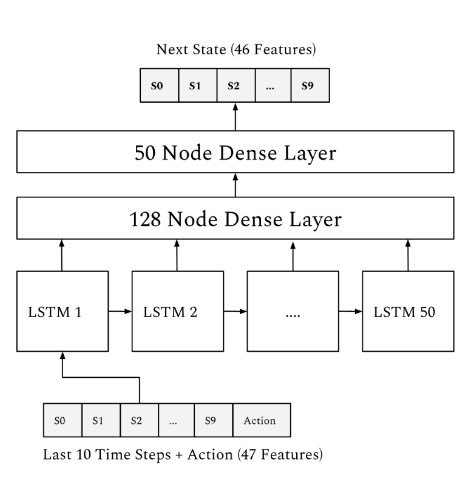
\includegraphics[width=\linewidth]{gymic.png}
    \caption{Neural architecture of GYMIC}
    \label{fig:gymic}
\end{figure}

\subsubsection{Reward model}

Highlighting the gravity of contracting sepsis, \emph{GYMIC} has only 2 outcomes: patient is discharged from intensive care or patient dies.
Its reward model reflects that, giving the agent a large positive or negative reward at the end of the episode, depending on the outcome.
However, in order to lower the difficulty of the simulator (delayed gratification makes training significantly harder \cite{delayedgrat-humans, delayedgrat-ai}) an additional reward is provided during the episode, based on the evolution of the patient's SOFA score \cite{sofa} - a commonly used measure of sepsis severity:

\begin{multline}
r\left(s_{t}, s_{t+1}\right)=C_{0} \mathbb{1}\left(s_{t+1}^{\mathrm{SOFA}}=s_{t}^{\mathrm{SOFA}} \& s_{t+1}^{\text {SOFA }}>0\right) + \\ +
C_{1}\left(s_{t+1}^{\mathrm{SOFA}}-s_{t}^{\mathrm{SOFA}}\right) + 
C_{2} \tanh \left(s_{t+1}^{\text {Lactate }}-s_{t}^{\text {Lactate }}\right)
\end{multline}

A third reward component is proposed to negatively reinforce action severity and encourage the agent to use low doses of drugs - an instance of \emph{confirmation bias} as discussed in section \ref{sec:bias}, but a necessary step given the issues in section \ref{sec:gymic-results}.

\subsubsection{Results and issues}
\label{sec:gymic-results}

Unfortunately, the experiments performed by the authors of \emph{GYMIC} indicate extreme overfitting.
Due to \emph{sampling bias} and simply inadequate size of the dataset there are treatments that have only occurred a few times in the training data and have always resulted in a positive health outcome.
In \emph{GYMIC} these treatments are silver bullets that guarantee a successful outcome while in real life they are risky and potentially very harmful.


\newpage
\chapter{An Artificial Paramedic} \label{ch:virtu-als}
\section{Virtu-ALS}
\label{sec:virtu-als}

\begin{figure}
    \centering
    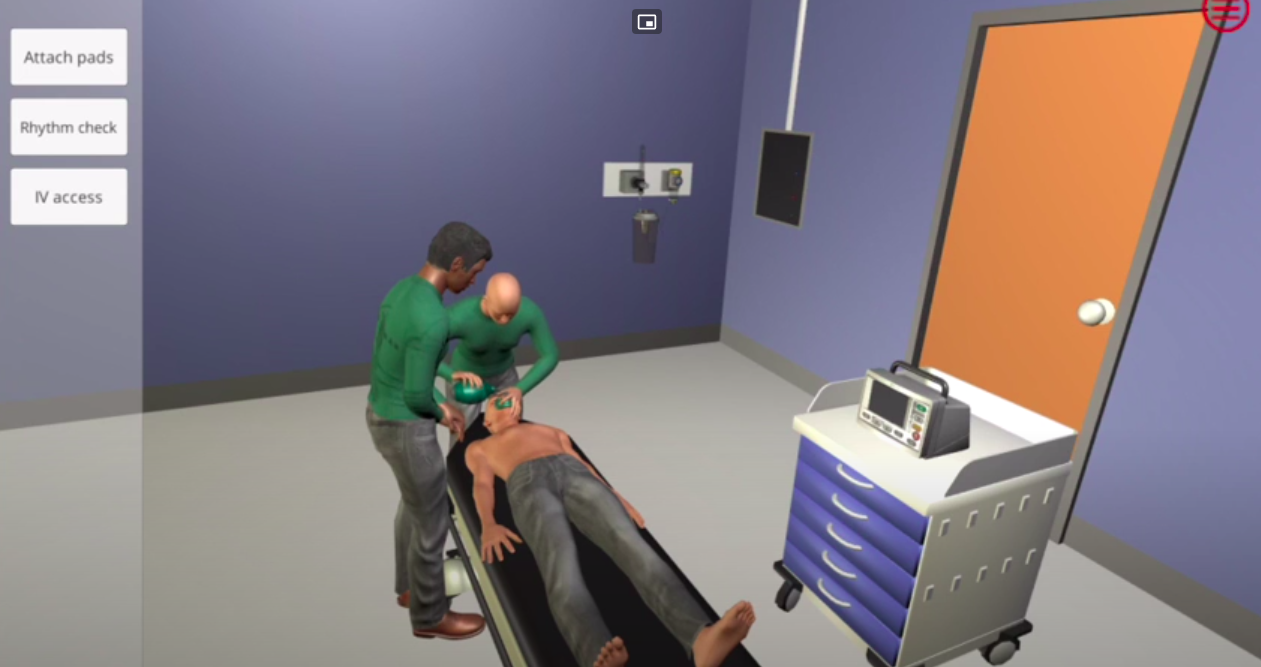
\includegraphics[width=\linewidth]{Virtu-ALS.png}
    \caption{Virtu-ALS}
    \label{fig:virtu-als}
\end{figure}

Virtu-ALS is a \emph{didactic} emergency care simulator mainly targeted at students and junior healthcare professionals, although its application as a reinforcement learning \emph{benchmark} was anticipated and accounted for by the authors \cite{virtu-als}.
Its most prominent feature is its visual nature (figure \ref{fig:virtu-als}): the user has access to a 3D-rendered virtual copy of a hospital room, view the monitor, press buttons on a defibrillator, etc.
However, the visual modality means that its observation space 
\begin{equation}
    \mathcal{O} \subset R^{307200}
\end{equation}

Such a high dimensionality of the observation space makes it an extremely challenging reinforcement learning task.
Tasks from this family have been solved with deep neural networks \cite{atari-rl}, however not only does it require a long and expensive training process, it also means that resulting treatment strategies are black box neural networks that no clinical expert understands.
This approach to decision making is extremely hard to introduce into clinical practice \cite{blackbox1,blackbox2}

Like most \emph{didactic} simulators, Virtu-ALS exhibits considerable \emph{confirmation bias} - any decision that's not supported by the standard emergency care protocol \cite{abcde,acls} is considered a mistake and rewarded negatively.

\section{Auto-ALS}

As our first model, we propose a low-dimensional version of \emph{Virtu-ALS}.
\emph{Auto-ALS} is a modification of Virtu-ALS that removes all the complexity of dealing with a visual 3D environment while retaining all the complexity of dealing with a patient that requires emergency care.
This is achieved by attaching an event listener to Virtu-ALS that registers all observable events that can occur in the simulator in response to the user's actions.
The events are listed in table \ref{tab:auto-als}, organized by which agent action can trigger which event.
\emph{Tick} is a special event that occurs every time the simulator is advanced a timestep, and is negatively reinforced, which when used with reinforcement learning algorithms discourages clinicaly unnecessary actions.

\texttt{MeasuredHeartRate, MeasuredRespRate, MeasuredCapillaryGlucose, MeasuredTemperature, MeasuredMAP, MeasuredSats, MeasuredResps} are \emph{measurements}, events that have a value $(\-infty; +\infty)$ associated with them.

\begin{table*}[]
\begin{tabular}{|p{0.4\linewidth}|p{0.45\linewidth}|c|}
\toprule
Agent actions &
  Patient reactions & Rewards
   \\
   \midrule
AssessResponse &
  ResponseVerbal,     ResponseGroan,     ResponseNone &
  \multirow{9}{*}{0} \\
AssessAirway &
  AirwayClear,     AirwayVomit,     AirwayBlood,     AirwayTongue &
   \\
AssessBreathing &
  BreathingNone,     BreathingSnoring,     BreathingSeeSaw,     BreathingEqualChestExpansion,     BreathingBibasalCrepitations,     BreathingWheeze,     BreathingCoarseCrepitationsAtBase,     BreathingPneumothoraxSymptoms,  VentilationResistance, \emph{MeasuredRespRate} &
   \\
AssessCirculation &
  RadialPulsePalpable,     RadialPulseNonPalpable, \emph{MeasuredHeartRate} &
   \\
AssessDisability &
  AVPU\_A,     AVPU\_U,     AVPU\_V, PupilsPinpoint,     PupilsNormal, \emph{MeasuredCapillaryGlucose} &
   \\
AssessExposure &
  ExposureRash,     ExposurePeripherallyShutdown,     ExposureStainedUnderwear, \emph{MeasuredTemperature} &
   \\
AssessDefibrillator &
   &
   \\
AssessMonitor &
  HeartRhythm0,     HeartRhythm1,     HeartRhythm2,     HeartRhythm3,     HeartRhythm4, \emph{MeasuredHeartRate}, \emph{MeasuredMAP}, \emph{MeasuredSats}, \emph{MeasuredResps} &
   \\
   DoNothing & & \\
   \midrule
ABG,     AirwayManoeuvres,     GiveAtropine,     GiveAdenosine,     GiveAdrenaline,     GiveAmiodarone,     GiveMidazolam,     Venflon,     Yankeur,     DrawBloods,     BPCuffOn,     BVM,     Guedel,     NRBMask,     DefibOn,     DefibAttachPads ,     DefibShock,     DefibCharge ,     DefibChangePaceCurrentDown,     DefibChangePaceCurrent,     DefibEnergyDown,     DefibEnergyUp,     DefibChangePaceRateDown,     DefibChangePaceRateUp,     DefibPace& 
   Blunder & $r_\text{blunder}$
   \\
   \midrule
   \multirow{2}{*}{Finish} & Failure & -1 \\
   & Success & 1 \\
   \midrule
   - & Tick & $r_\text{tick}$ \\
  \bottomrule
\end{tabular}
\caption{All actions and observations of Auto-ALS}
\label{tab:auto-als}
\end{table*}

    
The events in table \ref{tab:auto-als} only get registered if the agent has \emph{learnt} some piece of information, meaning that, for example, \verb|AirwayVomit| will only occur if the patient has vomit in their airway \emph{and} the agent checked the airway (which is part of the standard protocol \cite{abcde}).
Assessment skills (knowing where to look and how to establish the patient's state) are crucial for patient resuscitation, hence revealing all known health variables to the agent would jeopardize the simulation.


The observation vector in \emph{Auto-ALS} is based on all observations that have occurred between the beginning of the episode and current time.
However, more recent observations are more likely to still be relevant and should be given priority.
This is done with the following formula proposed in \cite{mpdp}:

\begin{equation}
     o^{+} = \langle o_1 \in O_1, \exp(t_1-t), \dots, o_n \in O_n, \exp(t_n-t), \rangle
\end{equation}

where $O_i$ is the value of the observation and $t$ is current time and $t_i$ is time when observation $i$ (for $i=5$, \verb|ResponseGroan|) has \emph{last} occurred and $\exp(t_i-t)$ represents its decaying relevance.
For \emph{measurements}, the $O_i$ equals the magnitude of the measurement, however, for binary obsevations $O_i$ would always be equal to one.
For memory efficiency, for all $i$ that correspond to binary observations, $O_i$ is skipped from the $o^{+} $ vector and the actual observation vector $o$ has size $36+7*2=50$, as opposed to $(36+7)*2=86$

See source code and documentation at \cite{auto-als}.


\newpage
\chapter{An Artificial Sonographer} \label{ch:imagym}
\section{Introduction}

Patient simulators are the cornerstone of clinical decision support solutions, providing a means to validate the efficacy of medical interventions in silico so cheaply that reinforcement learning algorithms can be used to develop protocols of clinical interventions automatically.
Unlike other machine learning applications, notably language modeling that can obtain a near-unlimited amount of data from the internet\footnote{See CommonCrawl \cite{commoncrawl} \url{commoncrawl.org}}, Healthcare suffers from an acute shortage of training data \cite{datashortage}.
As a result, many existing patient simulators are not trained on data from real patients, but instead rely upon expert knowledge \cite{towards}, leading to issues like \emph{confirmation bias} (the types of interventions currently favoured by clinical experts will work well in simulators developed by said experts irregardless of their real-world performance) and a high Sim2Real \cite{sim2real} gap.

In this work, we utilize a dataset of fetal ultrasound images to propose a novel data-driven patient simulator for decision support and automation in the field of obstetric ultrasonography \cite{obstetrics-sonography}.

The goal of this simulator is to accurately model the job of an ultrasound sonographer in the context of a patient undergoing a pregnancy in a way compatible with modern Reinforcement Learning methods \cite{rl-review}
to pave the way for autonomous or semi-autonomous ultrasound sonography \cite{autonomous-ultrasound-review}.
The job in question entails moving the ultrasound probe along the patient's body in order to acquire an image of the fetus that satisfies the guidelines for fetal-screening \cite{isoug-guidelines}, most importantly, the fact that the fetus' stomach and umbilical vein are on the image while their heart is not.

\newpage
\section{Methodology}

\paragraph{Dataset}

\begin{figure*}
    \centering
    \begin{subfigure}{.45\linewidth}
      \centering
      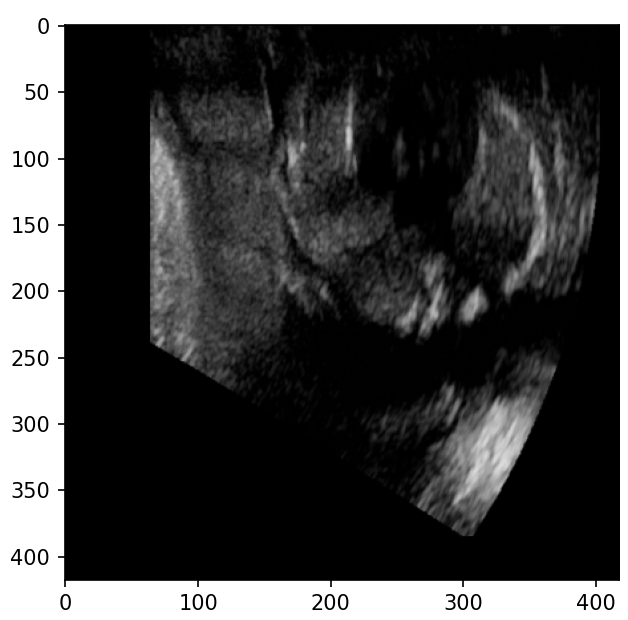
\includegraphics[width=.95\linewidth]{fetal_start.PNG}
      \caption{Starting point: the probe is located at the exact average of available positions. Heart, stomach and umbilical vein are unseen.}
      \label{fig:img-before}
    \end{subfigure}%
    \begin{subfigure}{.45\linewidth}
      \centering
      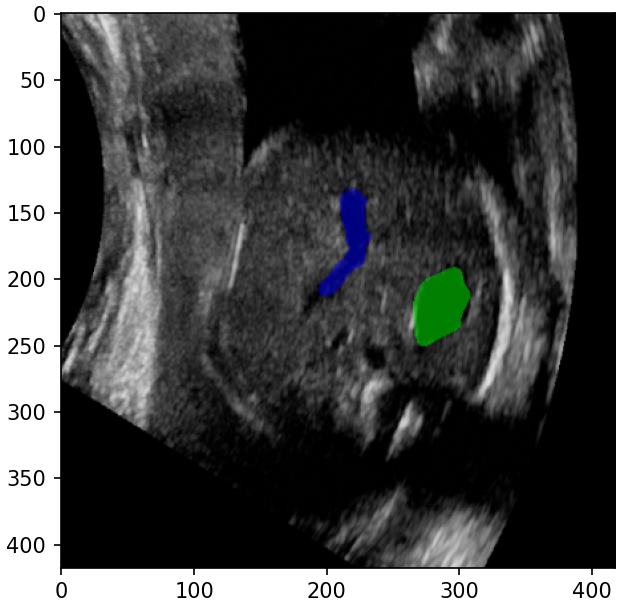
\includegraphics[width=.95\linewidth]{fetal_goal.PNG}
      \caption{Endpoint: stomach (green) and umbilical vein (blue) are present, heart is absent.}
      \label{fig:img-after}
    \end{subfigure}
    \caption{Two examples of the agent's observation at different positions of the probe}
    \label{fig:imgs}
\end{figure*}

The simulator is based on a dataset of 3D volumes representing fetal abdominal ultrasound scans (though be easily adapted to other medical imaging scenarios as long as a dataset of volumes and relevant organ annotations is available).
Each scan is a function defined over a cuboid $B$ of size $\langle x_\text{max},y_\text{max},z_\text{max} \rangle$ (in millimeters).
\begin{equation}
    I(x,y,z): B \rightarrow [0;1]
\end{equation}

Each scan is accompanied by three mask images $M_\text{heart}$, $M_\text{stomach}$ and $M_\text{uv}$ over the same domain, indicating which parts of the scan are considered to be the heart, the stomach and the umbilical vein respectively.

\begin{equation}
    M(x,y,z): B \rightarrow \{0,1\}
\end{equation}

\paragraph{Framework}

We adopt the industry-standard framework of {\em Episodic Partially Observable Markov Decision Process} \cite{kramerjdavidrPartiallyObservableMarkov1964, spaanPartiallyObservableMarkov2012}, implemented as OpenAI Gym \cite{gym} where every simulator is a 8-tuple of non-terminal state space $\mathcal{S}$, action space $\mathcal{A}$, observation space $\mathcal{O}$, stochastic observation model $\mathcal{O}, p_o(o | s, a)$, stochastic transition model $p_s(s_\text{next} | s_\text{prev}, a)$, stochastic reward model $p_r(r | s, a)$, initial state distribution $p_\text{init}(s)$ and episode termination model $p_\text{end}(s)$.

\paragraph{State}

The state, in this case, is the current position of the proble defined by 2 3-vectors, the position of the probe $s_\text{loc} \in \mathcal{S}_\text{loc}$ and its direction $s_\text{dir} \in R^{3}$.

The simulator has 2 modes for the space of possible locations $\mathcal{S}_\text{loc}$: \emph{free} and \emph{realistic} movement.
In \emph{free movement} mode, $\mathcal{S}_\text{loc} = B$, thus the agent can place the probe anywhere within the bounds of the image, even inside the patient.
In \emph{realistic movement} mode, $\mathcal{S}_\text{loc} \subset B$ representing the surface of the patient's body available to the agent.

\paragraph{Actions}

The action space $\mathcal{A} = R^{7}$, where any $a \in \mathcal{A}$ can be decomposed as

\begin{equation}
    a = (a_{x} , a_{y} , a_{z} , a_\text{roll} , a_\text{pitch} , a_\text{yaw}, a_\text{end})
\end{equation}

The first 3 components modify the $s_\text{loc}$, the next 3 modify $s_\text{dir}$ and, finally if $a_\text{end} > 0$, the episode terminates and the current image is considered final.
Note that in \emph{realistic movement} mode, blind application of $(a_{x} , a_{y} , a_{z})$ can lead to the probe being placed outside of the allowed domain of $\mathcal{S}_\text{loc}$.
In this case, a legal location will be chosen, in a manner that minimizes the distance between requested and real probe position:

\begin{equation}
    s_\text{loc} \leftarrow \min_{s \in \mathcal{S}_\text{loc}} \left\{ \lVert s - (s_\text{loc} + (a_{x} , a_{y} , a_{z})) \rVert \right\}
\end{equation}

\paragraph{Observations}

The observation is obtained by projecting $I(x,y,z)$ onto a plane defined by the current position of the probe $s_\text{loc}$ and its direction $s_\text{dir}$, simulating the image that the sonographer would see on their screen.
It is, theoretically, a function $I_\text{proj}(x_\text{proj}, y_\text{proj})$, however, since it is customary in POMDP framework for observations $o$ to be matrices, we replace it with a matrix of evaluations of $I_\text{proj}(x_\text{proj}, y_\text{proj})$ on an arbitrary (hyperparametrized) coordinate grid $\{(x_\text{proj}, y_\text{proj})\}$.

\paragraph{Rewards}

The quality of the image is defined in accordande with ISOUG guidelines \cite{isoug-guidelines} to be measured by the surface area of the heart, the stomach and the umbilical vein on the projection, normalized by the volume of these organs.

\begin{equation}
    Q(I_\text{proj}) = \frac{S_\text{stomach}(I_\text{proj})}{V_\text{stomach}(I)} + \frac{S_\text{heart}(I_\text{proj})}{V_\text{heart}(I)} + \frac{S_\text{uv}(I_\text{proj})}{V_\text{uv}(I)}
\end{equation}

The reward then is the diffence in quality between the current image and the one obtained at the previous iteration, so that probe movements that improve the image are rewarded positively and all rewards obtained during the episode sum up to the quality of the chosen image.

\newpage
\section{Related work}

Another simulator with a somewhat similar methodology is SonoRL \cite{sonorl}. The most important differences underlining the need for this simulator are:
\begin{itemize}
    \item SonoRL models ultrasonography of the spine (\emph{paramedian sagittal lamina view} \cite{spinal-guidelines}), while we focus on fetal screening.
    \item The reward function in SonoRL is a vector distance between the current position of the probe and the correct position. However, in reality, "correct" locations of the probe are numerous, comprising an equivalence class of solutions that satisfy the requirements in \cite{isoug-guidelines}.
    \item The implementation of SonoRL is not available to the wider community.
\end{itemize}

\newpage
\section{Future work}

One direction is to provide the observations in a low dimentional format.
At present, the neural network in charge of the agent is solving 2 separate tasks simultaneously: interpreting the image and making probe movement decisions based on it. Assigning this task to specialized components typically increases the agent's performance \cite{decoupling-rl}. Adding a feature extractor that will find relevant details in the image and replacing the image observation space with the space of these features would let the agent specialize purely in decision-making.

Besides, Healthcare automation raises specific concerns \cite{health-ai-explainability1,health-ai-explainability2} about the explainability of underlying models. 
As a way to make the agents more explainable, Programmatically Interpretable Reinforcement Learning \cite{pirl,neurogenetic} would be a logical extension of this work.


\newpage
\chapter{An Artificial Doctor} \label{ch:mimicseq}
%
\section{Introduction}

% What I would like to mention:
% RL as Sequence modeling, offline RL perspective
% Sequence modeling as a general paradigm
% The current state of Healthcare machine learning, lack of benchmarks, data subsets
% "Foundational model" buzzword


\paragraph{Intensive Care databases: a nano-review}
\label{sec:datasets}

% Why intensive care is a good source of data
Intensive Care is the medical speciality that supports patients whose lives are in immediate danger.
As such, it requires robust real time monitoring of the patient's vital signs due to quickly identify potential deterioration \cite{Bailey2013trial, Blount2010Real, Bockholt2022Real, Dimitrios1999Distributed, Fried2000Some, Mao2012integrated, Prgomet2016Vital, Vincent2018Improving}.
Monitoring hardware creates a datastream of variables like heart rate and blood oxygenation and, as a result, Intensive Care stands to benefit more than other fields of Healthcare from integration of data-driven models \cite{nunezreizBigDataAnalysis2019}.

% Datasets
MIMIC IV \cite{johnsonMIMICIVFreelyAccessible2023}, AmsterdamUMCdb \cite{amsterdamumcdb-a}, HiRID \cite{yecheHiRIDICUBenchmarkComprehensiveMachine} and the eICU Collaborative Research Database \cite{pollard2018a} are databases of health records obtained from Intensive Care Units.
Unlike many machine learning datasets, they avoid setting a standard for the parameters of the task such as which variables of a sample are to be used as features and which are to be predicted by the model, which samples are to be used for training and which are the holdout set - even what is a sample (a patient? an ICU admission? a drug? a diagnosis?). This makes them flexible and suitable for a wide array of tasks, but presents a challenge when seeking to compare different studies \cite{mcdermottReproducibilityMachineLearning2021}.

Derivative benchmarks, such as the MIMIC Benchmark \cite{harutyunyanMultitaskLearningBenchmarking2019} and HiRID-ICU-Benchmark \cite{yecheHiRIDICUBenchmarkComprehensiveMachine} seek to address the reproducibility issue: they put forth multiple datasets (one for each task) where all the information is derived from MIMIC and HiRID-ICU respectively, but is arranged specifically for the learning task at hand. They aim to become standard benchmarks for the tasks of mortality and length of stay prediction, patient fenotyping, prediction of circulatory, respiratory or kidney failure.

\paragraph{Towards foundation models for Healthcare}

Generalist models have demonstrated a superior performance to task specific models in many areas of machine learning \cite{reedGeneralistAgent2022} due to their ability to exploit implicit shared subtasks. 
This finding has precipitated the birth of a new paradigm known as foundation models \cite{zhouComprehensiveSurveyPretrained2023} - models trained on an all-encompassing dataset (such as the dataset that attempts to approximate all written text \cite{chelbaOneBillionWord2013}) and designed to be adapted to a broad array of specific downstream tasks.

The learning tasks typically studied in Healthcare are often interrelated. 
To use an example from section \ref{sec:datasets}, sepsis presents a high risk of death \cite{schlichtingRecognizingManagingSevere2007} and predicting sepsis is evidently useful for predicting mortality.
In light of existing research on generalist models, it is likely that considering them separately is counterproductive.
This, together with the vital societal importance of access to healthcare amidst understaffing \cite{ashleyy.metcalfHospitalUnitUnderstaffing2016, hudsonUnderstaffing2015, mercerMessageEditorinChief2008, munnUnderstaffingWardsCompromising2017, r.stanleyUnderstaffedOverwhelmed2010, SurveyShowsHidden1993, thelancetHealthcareSystemStaffing2018, UnderstaffingSignificantIssue2012} and population ageing \cite{2012health, Aslam2021Ageing, L1991aging, Lloyd2012Population, Mahishale2015Ageing, Mann2004aging, Sammy2019global, Suzman2015Health}, makes a foundation model for Healthcare a particularly important research goal.

\paragraph{The case for Healthcare as Sequence Modeling}
\label{sec:sequencemodel}

With a few notable exceptions foundation models tend to be sequence models: estimating the probability a sequence of fixed-size elements

\begin{equation}
    \hat{p}(t_1, \dots, t_n)
\end{equation}

typically modeled as conditional probability of one (usually last) element given others

\begin{equation}
    \hat{p}(t_n | t_1, \dots, t_n)
\end{equation}

since most tasks in machine learning can be represented as sequence modeling. 
There is evidence that this generality is a fundamental property of sequence models: see proofs that Recurrent Neural Networks \cite{siegelmannComputationTuringLimit1995} and Attention \cite{perezAttentionTuringComplete} are Turing-complete.

One of the tasks that has recently been reimagined as a Sequence Modeling task is Reinforcement Learning and Healthcare has a Reinforcement Learning interpretation: it's an interaction between the doctor (the agent) and the patient's body (the environment) that has all the trappings of a POMDP: the treatment interventions are actions $a_n$ and the observable vital signs are observations $o_n$.
Consider a \emph{trajectory} in a Partially Observable Markov Decision Process, i.e. a history of actions $a$, observations $o$ and rewards $r$:

\begin{equation}
    \tau = (o_1, a_1, r_1, o_2, a_2, r_2, o_3, a_3, r_3, \dots)
\end{equation}

A model $\hat{p}$ that can predict the next element in a trajectory can be used as a \emph{dynamics model} to predict the next observation from the patient:

\begin{equation}
    o_{n+1} \sim \hat{p}(o_{n+1} | \dots, o_n, a_n, r_n)
\end{equation}

as an \emph{imitative policy} to predict which intervention the doctor will choose next

\begin{equation}
    a_{n+1} \sim \hat{p}(a_{n+1} | \dots a_n, r_n, o_{n+1})
\end{equation}

or, after an additional optimization step, as an \emph{optimal policy} to predict which intervention the doctor \emph{should} choose next.
For a planning horizon of 1 (greedy policy) it is defined as:

\begin{equation}
    a_{n+1} = \arg \max_a \mathbb{E} [r_{n+1} \sim \hat{p}(r_{n+1} | \dots a_n, r_n, o_{n+1}, a)]
\end{equation}

Thus while the paradigm of Healthcare as a Sequence Modeling task is novel, there is a robust body of research reducing Healthcare to Reinforcement Learning \cite{yuReinforcementLearningHealthcare2021} and Reinforcement Learning to Sequence Modeling \cite{chenDecisionTransformerReinforcement2021, jannerOfflineReinforcementLearning2021, schmidhuberReinforcementLearningUpside2020}. 

\paragraph{Contributions}

In this paper we introduce
\begin{itemize}
    \item the paradigm of Healthcare as Sequence Modeling
    \item MIMIC-SEQ: a benchmark dataset for Sequence Models of Intensive Care derived from MIMIC-IV
    \item Evaluation guidelines for a holistic comparison of intensive care forecasting models
    \item An MLP-based baseline model
\end{itemize}

\newpage
\section{Related Work}

\cite{weiMIMICELMIMICIVEvent2022} develop MIMICEL, a linearized event sequence representation of MIMIC-IV-ED \cite{johnsonMIMICIVED2021} emergency department dataset for downstream application in machine learning and process mining. 
However, MIMIC-IV-ED is a smaller dataset than MIMIC-IV, and \cite{weiMIMICELMIMICIVEvent2022} stop short of releasing a full benchmark suite with an evaluation procedure and baselines.
Incorporating MIMICEL into MIMIC-SEQ would be a fruitful direction of future research.
Similarly to our approach,
\cite{kuznetsovaImportanceStepwiseEmbeddings2023} and \cite{tipirneniSelfSupervisedTransformerSparse2022} represent intensive care data as an irregular event stream timeseries, however they still rely on manual selection of important variables and prediction targets.

\section{MIMIC-SEQ}
\label{sec:dataset}

MIMIC-SEQ is a dataset for training foundational models for Intensive Care in the Sequence Modeling paradigm derived from MIMIC-IV.
It sets out a single machine learning task, with fully standardized train and test sets for reproducible comparisons between methods, while, at the same time, the task is so general that if a model accomplishes it successfully, this model can be used without fine-tuning for many narrow tasks, including mortality and length of stay prediction.
We also provide a suite of evaluation metrics and 2 baseline models.

%\begin{figure*}
%    \centering
%     \begin{subfigure}[b]{0.5\textwidth}
%         \includegraphics[width=\textwidth]{relationships.real.compact.png}
%         \caption{SQL schema of MIMIC}
%         \label{fig:mimic-schema}
%    \end{subfigure}
%     \hfill
%     \begin{minipage}[b]{0.45\textwidth}
%         \begin{subfigure}[b]{0.7\linewidth}
%             \includegraphics[width=\textwidth]{schema.drawio.png}
%             \caption{SQL schema of MIMIC-SEQ}
%             \label{fig:mimic-schema}
%         \end{subfigure}
%    \end{minipage}
%end{figure*}

\newpage
\section{Building the timeseries dataset}

\begin{figure}
    \centering
    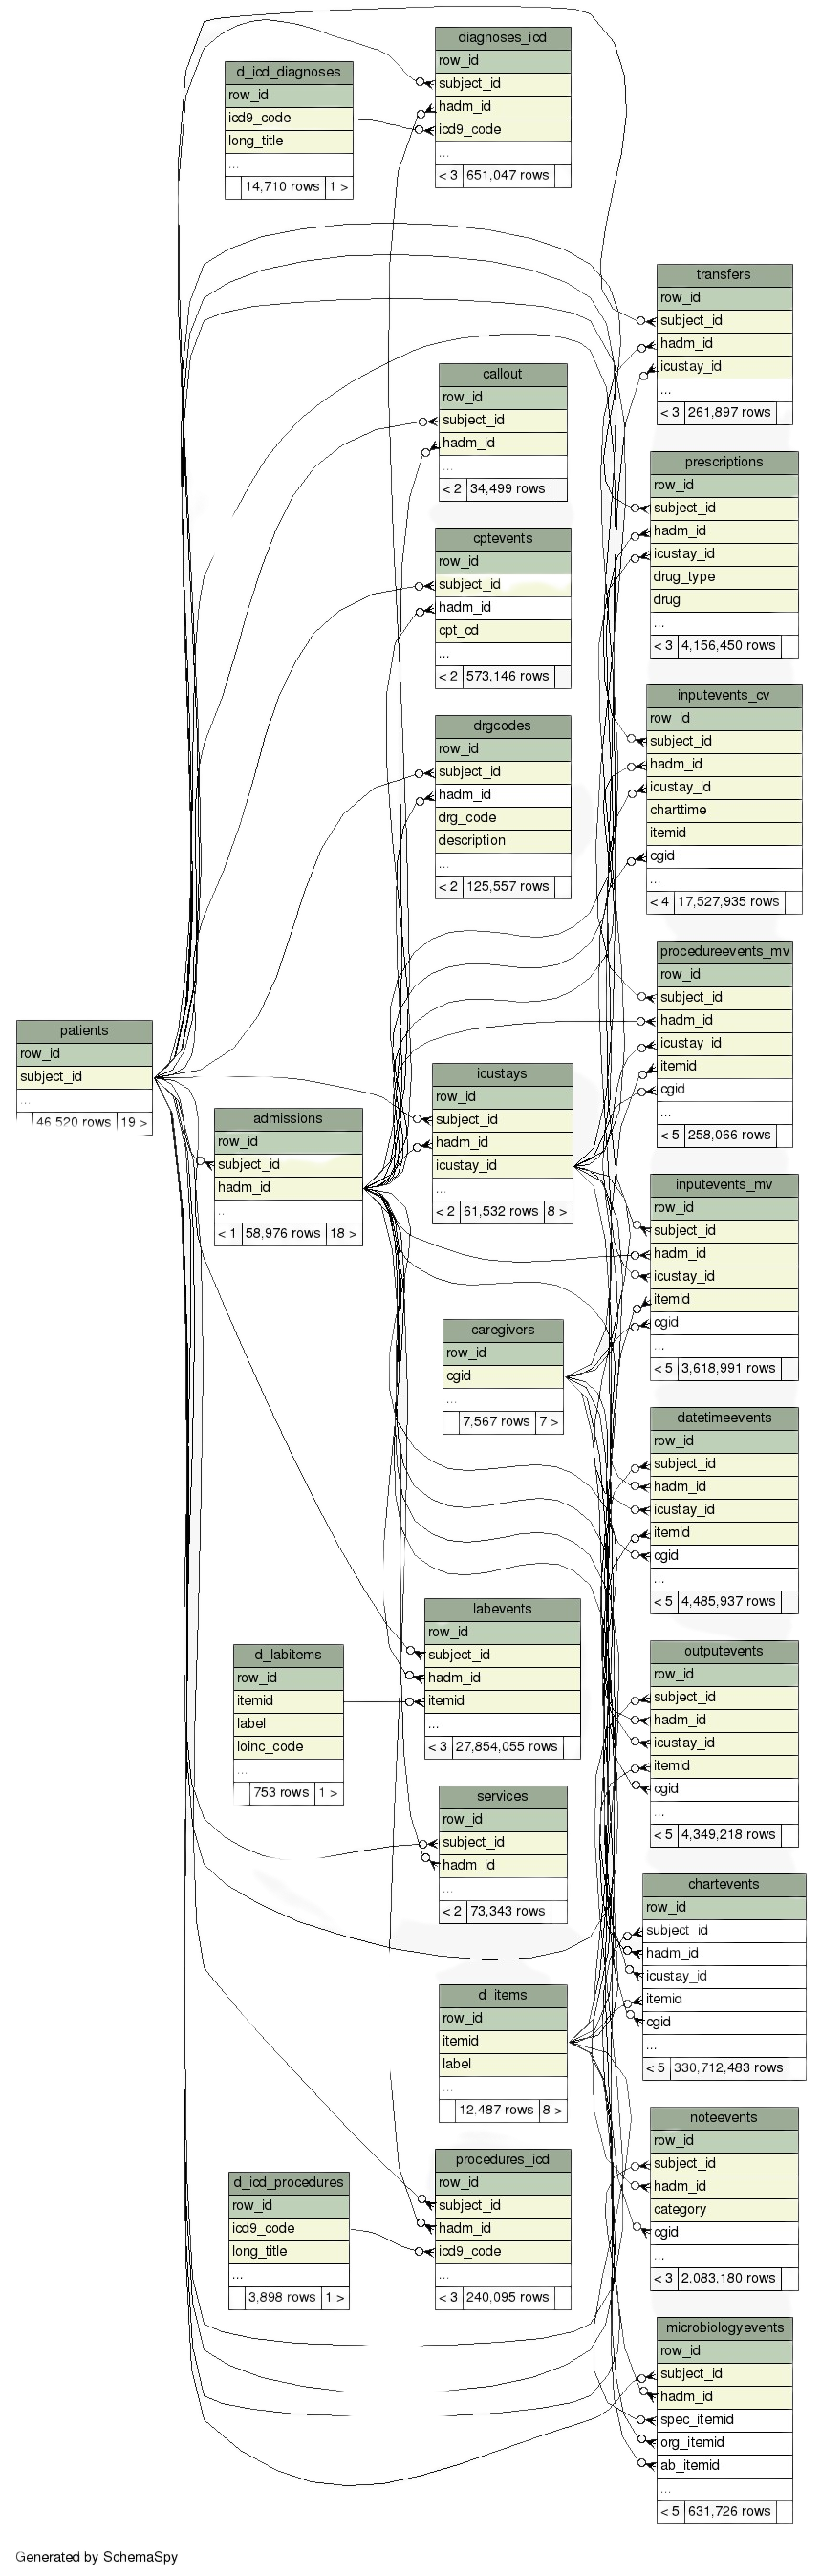
\includegraphics[width=0.8\linewidth]{mimiciv.png}
    \caption{Entity-Relationship diagram of MIMIC-IV}
    \label{fig:mimic}
\end{figure}

For every patient admission recorded in MIMIC-IV we collect all related information from various heterogeneous subdatasets, namely,

\begin{itemize}
    \item ICU input events (\texttt{inputevents})
    \item ICU procedures (\texttt{procedureevents})
    \item Hospital prescriptions (\texttt{prescriptions})
    \item Patient admissions and demographics (\texttt{admissions} and \texttt{patients})
    \item ICU charted events (\texttt{chartevents})
    \item Hospital lab events (\texttt{labevents})
    \item Microbiology tests (\texttt{microbiologyevents})
    \item Procedures coded in ICD format (\texttt{procedures\_icd})
    \item Healthcare Common Procedure Coding System (HCPCS) events (\texttt{hcpcsevents})
    \item Electronic medication administration records (eMAR) (\texttt{emar})
\end{itemize}

Every patient history is then represented as a sequence of events where each event has:
\begin{enumerate}
    \item a type (each type has an associated text label, i.e, "Penatal given")
    \item time when it happened
    \item (optionally) intensity
\end{enumerate}

Intensities may represent dosages of drugs or other quantitative measures (charted heart rate, blood pressure, patient age).

Events that have a duration, such as medication administrations, are recorded as 2 events: "start X" and "end X". 
Demographic information, including ethnicity, gender, and age, is recorded as a dummy event ocurring the time of admission.

\paragraph{Resulting dataset}

\begin{figure}
    \centering
    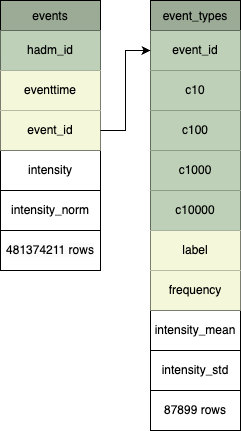
\includegraphics[width=0.7\linewidth]{mimicseq.png}
    \caption{Entity-Relationship diagram of MIMIC-SEQ}
    \label{fig:enter-label}
\end{figure}

\begin{table}[H]
    \centering
    \scriptsize
    \begin{tabular}{c|r|l}
    eventtime &	label &	intensity \\
    2185-08-13T16:57:00 &	WHITE	 & \\
    2185-08-13T16:57:00 &	AGE &	18.0 \\
    2185-08-13T16:57:00 &	URGENT ADMISSION &	 \\
    2185-08-13T16:57:00 &	FEMALE &	 \\
    2185-08-13T21:00:00 &	Start Prenatal Vitamins Tablet prescription, PO &	1.0 \\
    2185-08-13T22:00:00 &	Start LORazepam 1mg Tablet prescription, PO/NG &	 \\
    2185-08-13T22:00:00 &	Start HydrOXYzine 25 mg Tab prescription, PO/NG &	 \\
    2185-08-14T08:00:00 &	Start Complera 200 mg-25 mg-300 mg tablet prescription, ORAL &	1.0 \\
    2185-08-14T17:00:00 &	Start Acetaminophen 325mg Tablet prescription, PO/NG &	 \\
    2185-08-19T11:30:00 &	DISCHARGE TO HOME &	 \\
    2185-08-19T18:00:00 &	Stop LORazepam 1mg Tablet prescription, PO/NG &	 \\
    2185-08-19T18:00:00 &	Stop Prenatal Vitamins Tablet prescription, PO &	1.0 \\
    2185-08-19T18:00:00 &	Stop HydrOXYzine 25 mg Tab prescription, PO/NG &	 \\
    2185-08-19T18:00:00 &	Stop Complera 200 mg-25 mg-300 mg tablet prescription, ORAL &	1.0 \\
    2185-08-19T18:00:00 &	Stop Acetaminophen 325mg Tablet prescription, PO/NG &	 \\
    \end{tabular}
    \caption{An (unusually short) hospital admission from MIMIC-SEQ}
\end{table}

MIMIC-SEQ contains 481374190 clinical events in 522740 train and 10000 test episodes (hospital admissions).

\begin{table}[H]
    \centering
    \begin{tabular}{c|c|c|c}
         & min & avg & max \\
         Events per episode & 4 & 919 & 564721 \\
         Episode duration & 0 & 6 days & 68 years \\
    \end{tabular}
    \caption{Dataset statistics}
    \label{tab:stats}
\end{table}

It is publicly available, subject to (no cost, open to everyone) MIMIC-IV data use agreement.
See the dataset repository.

\paragraph{Clustering}

87899 event types is a very fine-grained view of the intensive care scenario that differentiates, for example, between different versions of the same drug (say, pills and tablets).
This is done intentionally to pave the way for sophisticated models, however, we recognize that a simplified version of the task can be helpful.
To that end, we enrich the dataset with 4 \emph{clusterings}: c10, c100, c1000 and c10000.
They are achieved by embedding each event type label with OpenAI's \emph{ada2} embedding model and running a k-means clustering algorithm in the induced latent space.
As a result, one can train a model for simplified \emph{clustered} versions the task making predictions in terms of broad event categories, not individual event types.

\paragraph{Evaluation guidelines}

We suggest evaluating forecasting models on 2 test tasks using the holdout patient histories:
\begin{description}
    \item[second day prediction] for every episode in the holdout set, use all events within 24 hours of the very first event as model input. Use the next 24 hours as expected output.
    \item[last day prediction] for every episode in the holdout set, use all events within 24 hours of the very last event as expected output. Use the rest of the events as model input. 
\end{description}

Each of the two can in turn be decomposed into:
\begin{description}
    \item[event prediction task] which events will happen and which will not?
    \item[intensity prediction task] if the event happens, what will be its intensity?
\end{description}

The former is a \emph{binary classification task} with metrics like \emph{accuracy}, \emph{precision} and \emph{recall}.
Note that it's a highly imbalanced binary classification task and, as such, relying on accuracy is not recommended - \emph{f1 score}, \emph{kappa} or \emph{dice score} shall be used instead.
The latter is a \emph{regression task} and the recommended metric is $R^2$ coefficient.

\emph{Event prediction} can be done in the space of concrete events or in the space of clusters c10, c100, c1000, c10000.
So, in total, a model evaluation includes 10 binary classification tasks (second day prediction and last day prediction for each event granularity) and 2 regression tasks.

\paragraph{Relationship to existing benchmarks}

A predictive model trained on \emph{MIMIC-SEQ} can perform the standard tasks used in current benchmarks \cite{harutyunyanMultitaskLearningBenchmarking2019}, such as
\begin{itemize}
    \item \emph{length of stay prediction} by estimating the probability of \texttt{DISCHARGE TO HOME} \\ \texttt{DISCHARGE TO REHAB} \\ \texttt{DISCHARGE TO HEALTHCARE FACILITY} \\ \texttt{DISCHARGE TO PSYCH FACILITY}\\\texttt{DISCHARGE TO OTHER FACILITY}\\\texttt{DISCHARGE TO REHAB}\\\texttt{DISCHARGE TO ASSISTED LIVING}\\\texttt{DISCHARGE TO HOSPICE}\\\texttt{DISCHARGE TO ACUTE HOSPITAL}\\\texttt{DISCHARGE AGAINST ADVICE} \\ \texttt{DISCHARGE TO HOME HEALTH CARE} \\ \texttt{DISCHARGE TO CHRONIC/LONG TERM ACUTE CARE} \\ \texttt{DISCHARGE TO SKILLED NURSING FACILITY} \\ \texttt{DISCHARGE TO DIED} \\ events over different timescales
    \item \emph{mortality prediction} by estimating the probability of \texttt{DISCHARGE TO DIED} relative to other types of discharge
    \item \emph{decompensation prediction} by estimate the probability of \texttt{DISCHARGE TO DIED} within 24 hours and/or events known to signify an acute increase in letality
    \item \emph{phenotyping} by estimating the probability of various \texttt{DISEASE X DIAGNOSED} events
\end{itemize}

as well as many others.

\newpage
\section{Baseline}
\label{sec:baseline}

Our baseline model consists of a two-layer multilayer perceptron (MLP) with 1000 hidden layer size RELU \cite{agarapDeepLearningUsing2018} activation function and batch normalization after each layer. As input, all events from the first day are used and one-hot encoded in a 87899-dimensional vector. As prediction target, all events from the second day are used and encoded via their clustering mapping, e.g. c10, c100, c1000, c10000, into a vector of the corresponding dimension. As objective function we used binary cross entropy. The last layer contains a sigmoid function which transforms the output to probabilities for each vector element. A threshold is set at 0.5 to decide if an event occurs or not. All models were trained with batch size 512 for 3 epochs.

We test our baseline on the \emph{second day event prediction task} and summarize the results for different clusterings in table \ref{tab:mytable2}. It can be seen that the more classes are in the clustering, the harder the prediction task becomes. As noted above, accuracy is a deceptive metric in this scenario.

\begin{table}[H]
  \centering
    \begin{tabular}{lcccc} \toprule
        {clustering} & {recall} & {accuracy} & {precision} & {F1}  \\ \midrule
        {c10}  & 0.903 & 0.840 & 0.790 & 0.827 \\
        {c100}  & 0.568 & 0.885 & 0.713 & 0.632 \\
        {c1000}  & 0.500  & 0.976 & 0.710  & 0.586 \\
        {c10000}  & 0.509  & 0.996 &  0.703  & 0.589 \\ \midrule
%        {average performance}  & \textbf{0.598}  & -0.597 & 0.598  & 0.052 \\ \bottomrule
    \end{tabular}
  \caption{Evaluation results of 2 x 1000 MLP for first day - second day  prediction, entire dataset}
  \label{tab:mytable2}
\end{table}



For many patients it is the case that they are in the hospital for only one day. For these patients, the model should predict no event on the second day. However, evaluation of the models showed that this is almost never the case. However, one can argue that it is more important to get problematic patients correct than the ones who leave the hospital after one day. Therefore, we evaluated the model also only on patients which are in the hospital for at least 2 days. Since the data is roughly ordered according to length of stay, we achieved this by skipping the first 100k samples in the training and the first 1k samples in the test data. The models shows improved performance here, as can be seen in Table \ref{tab:mytable1}.


\begin{table}[H]
  \centering
    \begin{tabular}{lcccc} \toprule
        {clustering} & {recall} & {accuracy} & {precision} & {F1}  \\ \midrule
        {c10}  & 0.942  & 0.854 & 0.850  &  0.890 \\ 
        {c100}  & 0.633  & 0.878 & 0.765  &  0.692 \\ 
        {c1000}  & 0.548  & 0.974 & 0.770  &  0.640 \\ 
        {c10000}  &  0.539  & 0.995 & 0.771  &  0.634 \\ \midrule
        
%        {average performance}  & \textbf{0.598}  & -0.597 & 0.598  & 0.052 \\ \bottomrule
    \end{tabular}
  \caption{Evaluation results of 2 x 1000 MLP for first day - second day  prediction, skipping first 100k train / 1k test samples}  \label{tab:mytable1}
\end{table}


%\begin{table}[h]
%  \centering
%    \begin{tabular}{lcccc} \toprule
%        {c10000} & {recall} & {accuracy} & {precision} & {F1}  \\ \midrule
%        {entire dataset}  & 0.495  & 0.996 & 0.711  &  0.583 \\ \midrule
%        {average performance}  & \textbf{0.598}  & -0.597 & 0.598  & 0.052 \\ \bottomrule
%    \end{tabular}
%  \caption{Evaluation results of 2 x 1000 MLP for first day - second day  prediction with c10000 for different subsets, run again!}  \label{tab:mytable}
%\end{table}

The same setup but with 3 hidden layers and 5000 units each shows improved performance as can be seen in table \ref{tab:mytable3}. Bigger models were tested as well, but showed no further improvement.


\begin{table}[H]
  \centering
    \begin{tabular}{lcccc} \toprule
        {configuration} & {recall} & {accuracy} & {precision} & {F1}  \\ \midrule
        {1}  & 0.505  & 0.996 &  0.727  & 0.595 \\
        {2} & 0.544  & 0.9959 &  0.784  & 0.642 \\  \midrule
%        {average performance}  & \textbf{0.598}  & -0.597 & 0.598  & 0.052 \\ \bottomrule
    \end{tabular}
  \caption{All evaluations with c10000; 1: Evaluation results of 3 x 5000 MLP for first day - second day  prediction, entire dataset; 2: Evaluation results of 3 x 5000 MLP for first day - second day prediction, skip first 100k train / 1k test samples}
  \label{tab:mytable3}
\end{table}




Replacing ones in the one-hot encoding with the corresponding events' intensities impaired the models' performance, likely because it introduces a false equivalency between a zero-intensity event and lack of an event, i.e. "average blood pressure" is different from "no blood pressure measurement".

% \begin{table}[h]
%   \centering
%     \begin{tabular}{SSSSSSSS} \toprule
%         {clustering} & {recall} & {accuracy} & {precision} & {F1}  \\ \midrule
%         {c10000}  & 0.339  & 0.995 &  0.687  & 0.452 \\ \midrule
% %        {average performance}  & \textbf{0.598}  & -0.597 & 0.598  & 0.052 \\ \bottomrule
%     \end{tabular}
%   \caption{Evaluation results of 2 x 1000 MLP for first day - second day  prediction, 500k dataset with intensity values}
%   \label{tab:mytable}
% \end{table}


\newpage
\section{Conclusion}

Narrow tasks in machine learning for intensive care have been a result of technical limitations that have become less relevant with recent advances in the field. 
We propose a more general approach, publish a dataset to support it and demonstrate its viability with a simple baseline model.
The long term ambition of this work is to become the basis for training foundation models of intensive care using modern neural network architectures.
Of particular interest are Transformers \cite{vaswaniAttentionAllYou2023}, Neural Controlled Differential Equations \cite{kidgerNeuralControlledDifferential2020} and Structured State Space Models \cite{guEfficientlyModelingLong2022}.

\newpage
\chapter{Appendices}

\chapter{Reproducibility and software artefacts}

\section{FizzBuzzLM}

\section{Cibi}

\section{tree2tree}

\section{programlib}

\section{SEIDR}

\section{imagym}

\section{Auto-ALS}

\epigraph{Стёр строк больше, чем выдал Джон Гришам \\ Нос тёр жёстче разве что Жижек}{Oxxxymiron}

This project has received funding from European Union’s Horizon 2020 research and innovation programme under grant agreement n° 812882. 

Parts of this text were converted from spoken audio with the use of English-only medium size OpenAI Whisper model \cite{radfordRobustSpeechRecognition2022}

\newpage
\chapter{Acknowledgments}

Parts of this text were converted from spoken audio with the use of English-only medium size OpenAI Whisper model \cite{radfordRobustSpeechRecognition2022}

\printbibliography

\end{document}
